%----------------------------------------------------------------------------------
% Exemplo do uso da classe pucrs-ppgcc.cls. Veja o arquivo .cls
% para mais detalhes e instruções.
%----------------------------------------------------------------------------------

% Seleção de idioma da monografia. Por enquanto as únicas opções
% suportadas são 'portuguese' e 'english'
% Para impressão em frente e verso, use a opção 'twoside'. Da
% mesma forma, use 'oneside' para impressão em um lado apenas.
%\documentclass[portuguese,twoside]{pucrs-ppgcc}
\documentclass[english,twoside]{pucrs-ppgcc}

%----------------------------------------------------------------
% Coloque seus pacotes abaixo.
%
% Obs.: muitos pacotes de uso comum do LaTeX, como amsmath,
% geometry e url já são automaticamente incluídos pela classe
% (veja o arquivo .cls). Isso torna obrigatória a presença destes
% no sistema para o uso desta classe, mas ao mesmo tempo o uso se
% torna mais simples.  Recomendo a instalação da versão mais
% recente da distribuição TeXLive (para Windows e UNIXes):
% www.tug.org/texlive/
%
% Pacotes e opções já incluídas automaticamente:
%
% \RequirePackage[T1]{fontenc}[2005/09/27]
% \RequirePackage[utf8x]{inputenc}[2008/03/30]
% \RequirePackage[english,brazil]{babel}[2008/07/06]
% \RequirePackage[a4paper]{geometry}[2010/09/12]
% \RequirePackage{textcomp}[2005/09/27]
% \RequirePackage{lmodern}[2009/10/30]
% \RequirePackage{indentfirst}[1995/11/23]
% \RequirePackage{setspace}[2000/12/01]
% \RequirePackage{textcase}[2004/10/07]
% \RequirePackage{float}[2001/11/08]
% \RequirePackage{amsmath}[2000/07/18]
% \RequirePackage{amssymb}[2009/06/22]
% \RequirePackage{amsfonts}[2009/06/22]
% \RequirePackage{url}
% \RequirePackage[table]{xcolor}[2007/01/21]
%----------------------------------------------------------------
% Para inserção de figuras.
\usepackage{graphicx}
% Utilize a opção 'pdftex' se você estiver usando o pdflatex (que
% permite figuras em formatos como .jpg ou .png)
%\usepackage[pdftex]{graphicx}

% Para tabelas com elementos ocupando mais de uma linha
\usepackage{multirow}
% Para frações na mesma linha (ex. ⅓).
\usepackage{nicefrac}
% Para inserir figuras lado a lado.
% \usepackage{subfigure}
% Para formatar algoritmos.
% A opção [algo2e] é necessária para evitar conflitos
% com as definições da classe.
%\usepackage[algo2e]{algorithm2e}
\usepackage{algorithmic}
% Um float do tipo algoritmo. No momento
% este pacote é incompatível com a classe.
%\usepackage{algorithm}

\usepackage{caption}
\usepackage{subfigure}
\usepackage{amsthm}
\usepackage{amsmath}
\newtheorem{thm}{Theorem}
\usepackage{listings}
\usepackage{rotating}
\usepackage{tablefootnote}




%----------------------------------------------------------------
% Autor (OBRIGATÓRIO)
%----------------------------------------------------------------
\author{Carlos Roberto Moratelli}

%----------------------------------------------------------------
% Título (OBRIGATÓRIO). Devem ser passados DOIS parâmetros,
% o título em português E o inglês, não importando o idioma
% escolhido. Os títulos são utilizados para a montagem da capa,
% resumo e abstract mais tarde.
%----------------------------------------------------------------
\title{Uma camada leve de virtualização assistida por hardware para sistemas embarcados}
      {A lightweight virtualization layer with hardware-assistance for embedded systems}

%----------------------------------------------------------------
% Opções para o tipo de trabalho (OBRIGATÓRIO)
%----------------------------------------------------------------
%\tipotrabalho{\monografia}  % Monografias em geral (e de "bônus": TCCs)
%\tipotrabalho{\pep}         % Plano de estudo e pesquisa
%\tipotrabalho{\dissertacao} % Dissertação
%\tipotrabalho{\ptese}       % Proposta de tese
\tipotrabalho{\tese}         % Tese

%----------------------------------------------------------------
% Seleção do curso ("este trabalho é um requisito parcial para
% obtenção do grau de (mestre ou doutor) em Ciência da Computação").
% Necessário somente para o tipo 'monografia'.
%----------------------------------------------------------------
%\grau{\bacharel} % Este é "bônus"
%\grau{\mestre}
\grau{\doutor}

%----------------------------------------------------------------
% Orientador (e Co-orientador, caso haja um). É OBRIGATÓRIO
% informar pelo menos o orientador.
%----------------------------------------------------------------
\orientador{Fabiano Hessel}
%\coorientador{Ciclano de Farias}

%----------------------------------------------------------------
% A capa é inserida automaticamente. Por isso não é necessário
% chamar \maketitle
%----------------------------------------------------------------
\begin{document}

%----------------------------------------------------------------
% Depois da capa vem a dedicatória e a epígrafe.
%----------------------------------------------------------------
\dedicatoria{To my family and friends.}

%\epigrafe{Talk is cheap. Show me the code.}
\epigrafe{I'm doing a (free) operating system (just a hobby, won't be big and professional like gnu) for 386(486) AT clones.}
         {Linus Torvalds}

%----------------------------------------------------------------
% Também dá para fazer as duas na mesma página:
%----------------------------------------------------------------
%\dedigrafe{Dedico este trabalho a meus pais.}
%          {The art of simplicity is a puzzle of complexity.}
%          {Douglas Horton}

%----------------------------------------------------------------
% A seguir, a página de agradecimentos (OPCIONAL):
%----------------------------------------------------------------
\begin{agradecimentos}

I would like to express my sincere gratitude to those who helped me throughout all my Ph.D. years and made this dissertation possible. First of all, I would like to thank my advisor, Prof. Fabiano Passuelo Hessel, who has given me the opportunity to undertake a Ph.D. and provided me invaluable guidance and support in my Ph.D. and in my academic life in general. Thank you to all the Ph.D. committee members – Prof. Carlos Eduardo Pereira (dissertation proposal), Prof. Rodolfo Jardim de Azevedo, Prof. Rômulo Silva de Oliveira and Prof. Tiago Ferreto - for the time invested and for the valuable feedback provided.Thank you Dr. Luca Carloni and the other SLD team members at the Columbia University in the City of New York for receiving me and giving me the opportunity to work with them during my ‘sandwich’ research internship. 

Eu gostaria de agraceder minha esposa, Ana Claudia, por ter estado ao meu lado durante todo o meu período de doutorado. O seu apoio e compreensão foram e continuam sendo muito importantes para mim. Obrigado pela paciência, amor e carinho durante todos esses anos. Também gostaria de agradecer aos meus pais e irmão pelo apoio durante toda a minha vida. Agradeço aos colegas e amigos do laboratório GSE/PUCRS, especialmente ao amigo Sergio Johann Filho pelas importantes discusões durante a execução do trabalho. 



\end{agradecimentos}

%----------------------------------------------------------------
% Resumo, com as palavras-chave passadas por parâmetro
% (OBRIGATÓRIO, ao menos para teses e dissertações)
%----------------------------------------------------------------
\begin{resumo}{Virtualização, Sistemas Embarcados, Hypervisor, Tempo-real}
\vspace{-3.6cm}
O poder de processamento presente nos sistemas embarcados modernos permite a adoção de técnicas de virtualização. Juntamente com os ganhos em redução de custo e melhor utilização dos recursos, como por exemplo uma melhor utilização do processador, a virtualização possibilita a co-execução de diferentes sistemas operacionais em um processador, sejam eles sistemas operacionais de tempo real (RTOS) e/ou de propósito geral (GPOS). 
%Um sistema virtualizado pode herdar o tempo de resposta deterministico do RTOS e toda a base de software do GPOS. 
A implementação da técnica de virtualização esta baseada em um módulo de software denominado hypervisor. %O hypervisor deve ser cuidadosamente projetado para que seja possível extrair o máximo das vantagens da virtualização.

Devido a complexidade de se desenvolver uma nova camada de virtualização especialmente projetada para sistemas embarcados, muitos autores propuseram modificações em sistemas de virtualização que são largamente empregados em servidores na nuvem para melhor adapta-los às necessidades dos sistemas embarcados. Contudo, a utilização de memória e os requisitos temporais de alguns dispositivos embarcados requerem abordagens diferentes daquelas utilizadas em servidores. Além disso, a atual tendência de utilização de virtualização nos dispositivos projetados para a internet das coisas (do inglês Internet of Things - IoT) aumentou o desafio por hypervisors mais eficientes, em termos de memória e processamento. Estes fatores motivaram o surgimento de diversos hypervisors especialmente projetados para atender os requisitos dos atuais sistemas embarcados. 

Nesta tese, investigou-se como a virtualização embarcada pode ser melhorada a partir de seu estado atual de desenvolvimento para atender as necessidades dos sistemas embarcados atuais. Como resultado, propõe-se um modelo de virtualização capaz de agregar os diferentes aspectos exigidos pelos sistemas embarcados. O modelo combina virtualização completa e para-virtualização em uma camada de virtualização híbrida, além da utilização de virtualização assistida por hardware. Uma implementação baseada neste modelo é apresentada e avaliada. Os resultados mostram que o hypervisor resultante possui requisitos de memória compatíveis com os dipositivos projetados para IoT. Ainda, GPOSs and RTOS podem ser executados mantendo-se o isolamento temporal entre eles e com o baixo impacto no desempenho. 
\end{resumo}

%----------------------------------------------------------------
% Abstract, com as palavras-chave passadas por parâmetro
% (OBRIGATÓRIO, ao menos para teses e dissertações)
%----------------------------------------------------------------
\begin{abstract}{Virtualization, Embedded Systems, Hypervisor, Real-time}


\vspace{-3cm}
The current processing power of modern embedded systems enable the adoption of virtualization techniques. In addition to the direct relationship with cost reduction and better resource utilization, virtualization permits the integration of real-time operating systems (RTOS) and general-purpose operating systems (GPOS) on the same hardware system. The resulting system may inherit deterministic time response from the RTOS and a large software base from the GPOS. However, the hypervisor must be carefully designed. 

Due to the complexity of developing a virtualization layer designed specially for embedded systems from scratch, many authors have proposed modifications of the widely used server virtualization software to better adapt it to the particular needs of embedded system. However, footprint and temporal requisites of some embedded devices require different approaches than those used in server farms. Also, currently virtualization is being adapted for the field of the Internet of Things (IoT), which has increased the challenge for more efficient hypervisors. Thus, a generation of hypervisors focused on the needs of embedded systems have emerged . 

This dissertation investigated how embedded virtualization can be improved, starting from the current stage of its development. As a result, it is proposed a virtualization model to aggregate different aspects required by embedded systems. The model combines full and para-virtualization in a hybrid virtualization layer. In addition, it explores the newer features of embedded processors that have recently adopted hardware-assisted virtualization. A hypervisor implementation based on this model is presented and evaluated. The results show that the implemented hypervisor has memory requirements compatible with devices designed for IoT. Moreover, general-purpose operating systems and real-time tasks can be combined while keeping them temporally isolated. Finally, the overall virtualization overhead is for most part lower than in other embedded hypervisors.
\end{abstract}

%----------------------------------------------------------------
% Listas e sumário, nessa ordem. Somente o sumário é obrigatório,
% portanto, comente as outras listas, caso sejam desnecessárias.
%----------------------------------------------------------------
\listoffigures       % Lista de figuras      (OPCIONAL)
\listoftables        % Lista de tabelas      (OPCIONAL)
%\listofalgorithms    % Lista de algoritmos   (OPCIONAL)
\listofacronyms      % Lista de siglas       (OPCIONAL)
%\listofabbreviations % Lista de abreviaturas (OPCIONAL)
%\listofsymbols       % Lista de símbolos     (OPCIONAL)
\tableofcontents     % Sumário               (OBRIGATÓRIO)

%----------------------------------------------------------------
% Aqui começa o desenvolvimento do trabalho. Para uma melhor
% organização do documento, separe-o em arquivos,
% um para cada capítulo. Para isso, utilize o comando \include,
% como mostrado abaixo.
%----------------------------------------------------------------

\sigla{ABI}{Application Binary Interface}
\sigla{ADPCM}{Adaptive Differential Pulse-code Modulation}
\sigla{ADU}{Application Domain Unit}
\sigla{API}{Application Programming Interface}
\sigla{BEC}{Best Execution Case}
\sigla{BE-VCPU}{Best-effort Virtual Central Processing Unit}
\sigla{BVT}{Borrowed Virtual Time}
\sigla{CBS}{Constant Bandwidth Server}
\sigla{CE}{Costumer Electronic}
\sigla{CPU}{Central Processing Unit}
\sigla{CP0}{Coprocessor 0}
\sigla{CSA}{Compositional Scheduling Architecture}
\sigla{DMA}{Dynamic Memory Access}
\sigla{DPR}{Dynamic Partial Reconfiguration}
\sigla{DRAM}{Dynamic Random-Access Memory}
\sigla{EDF}{Earliest Deadline First}
\sigla{ES}{Embedded System}
\sigla{FP}{Fixed Priority}
\sigla{FV}{Full-Virtualization}
\sigla{GCP0}{Guest Cooprocessor 0}
\sigla{GPOS}{General Purpose Operating System}
\sigla{GSE}{Embedded Systems Group}
\sigla{GSM}{Global System for Mobile Communications}
\sigla{GuestCtl0}{Guest Control Register 0}
\sigla{HAL}{Hardware Abstraction Layer}
\sigla{HLL}{High Level Languages}
\sigla{HVM}{Hardware-assisted Virtualization}
\sigla{IASim}{MIPS Instruction Accurate Simulator}
\sigla{IoT}{Internet of Things}
\sigla{IPA}{Intermediate Physical Address}
\sigla{ISA}{Instruction Set Architecture}
\sigla{I/O}{Input/Output}
\sigla{IOMMU}{Input–output Memory Management Unit}
\sigla{JVM}{Java Virtual Machine}
\sigla{NVRAM}{Non-Volatile Random Access Memory}
\sigla{OS}{Operating System}
\sigla{OVP}{Open Virtual Platforms}
\sigla{PA}{Physical Address}
\sigla{PID}{Processor Identification}
\sigla{PV}{Para-Virtualization}
\sigla{RTM}{Real-time Manager}
\sigla{RTOS}{Real-time Operating System}
\sigla{RT-VCPU}{Real-time Virtual Central Processing Unit}
\sigla{SEDF}{Simple Earliest Deadline First}
\sigla{USB}{Universal Serial Bus}
\sigla{VA}{Virtual Address}
\sigla{VCPU}{Virtual Central Processing Unit}
\sigla{VHH}{Virtual Hellfire Hypervisor}
\sigla{VM}{Virtual Machine}
\sigla{VMM}{Virtual Machine Manager}
\sigla{WEC}{Worst Execution Case}






\simbolo{C}{Capacity for EDF algorithm}
\simbolo{D}{Deadline for EDF algorithm}
\simbolo{KB}{kilobyte}
\simbolo{MB}{Megabyte}
\simbolo{MHz}{MegaHertz}
\simbolo{P}{Period for EDF algorithm}
\simbolo{U}{CPU utilization for EDF algorithm}













\chapter{\label{chapter:intro}Introduction}

Embedded systems are being widely adopted in all areas of human activity. Their increased performance during recent years has enabled a wide range of new applications. However, more processing power implies more functionalities and increased software complexity, which directly impacts the design constraints and goals of embedded systems \cite{sisu2014}. For example, the possibility for the final user to develop and download new applications, before exclusively found in general-purpose systems, can now be found in many modern embedded devices \cite{HeiserRole}. This scenario has forced designers and companies to adopt new strategies, such as increased use of software layers allowing for more flexible platforms capable of meeting timing, energy consumption, and time-to-market constraints. Although embedded systems are assuming many of the features of general-purpose systems, some differences remain. They present critical real-time constraints and frequently have resource constraints such as, limited battery, memory and processing power. 

The appearance of server farms in the 1990s and the increasing performance of the computer systems stimulated the adoption of virtualization. Virtualization allows for the possibility of decoupling the one-to-one correspondence between hardware and software. Thus, keeping several different operating systems on the same computer system, can drastically reduce the maintenance and energy costs \cite{muench2014}.  Different operating systems reside in a shared memory and are combined on a single or multi-core processor through a software stack called a virtual machine monitor or hypervisor. In recent years,  virtualization technology has quickly moved towards embedded systems motivated by the increasing processing power of the embedded processors and the increasing challenges to comply with their requirements. Although server virtualization is a well-known and mature technology widely applied for commercial use, embedded system virtualization is still being studied and developed. The main restriction to broader use of virtualization for embedded systems is that their requirements differ from server and enterprise systems \cite{Sandtrom2013}. Most notably, timing constraints and limited resources, like CPU and memory, are the main concerns around embedded systems virtualization. Thus, virtualization as deployed in the enterprise environment cannot be directly used in embedded systems. 

There are many studies proposing different techniques for embedded system virtualization. A common approach is to adapt hypervisors widely used in server virtualization to embedded systems. The main concern about general purpose hypervisors is the absence of suitable support for real-time and memory requirements incompatible with some embedded devices. Despite these limitations, researchers are continually working to improve the embedded support of open-source hypervisors for server virtualization, like XEN and KVM, as seen in \cite{Dall2014}, \cite{Dan2015}, \cite{seehwan2014} and \cite{avanzini2015}. On the other hand, the distinguished characteristics of the embedded systems have motivated the appearance of hypervisors specially designed for embedded virtualization. Among the goals for embedded hypervisors development, two of them are frequently addressed: to keep low memory requirements and some level of support for real-time applications. Additionally, the diversity of embedded systems and their applications encourages the development of many different embedded hypervisors, like SPUMONE \cite{spumone2008}, Xtratum \cite{trujillo2013}, M-Hypervisor \cite{rui2013}, Xvisor \cite{patel2015} and the L4 hypervisors family \cite{Xia2015}, \cite{Heiser2010}, \cite{pikeos}, \cite{yang2011}.

Intel and AMD manufactures provided hardware support for virtualization on the x86 architecture to address the continuous adoption of server virtualization. This was aimed  to simplify the virtualization software layer and to improve performance. Before hardware-assisted virtualization, hypervisors needed to implement a technique called para-virtualization that consists of modifying the operating system to be virtualized. These operating system modifications break the software compatibility and require additional engineering work along with licence and source-code access for proprietary software. With dedicated hardware for virtualization, the hypervisors could implement a technique called full-virtualization where no modifications are required on the target operating system. Thus, making it easier to support new operating systems, especially proprietary ones. Similar to the x86 architecture, the late adoption of hardware-assisted virtualization for embedded processors made para-virtualization rule the development of embedded virtualization. Nowadays, the main embedded processor manufacturers had already designed virtualization extensions for their processor families, like PowerPC \cite{powerpcvz}, ARM \cite{armvt} and MIPS \cite{mipsvz}. These gave hypervisor developers more design choices. Modern hardware-assisted virtualization now makes it possible to virtualize an operating system without any modification and keeps performance close to the level of non-virtualized systems. This is important to support legacy software. However, advanced hypervisor features like communication among virtual machines or shared devices may still require para-virtualization technique. 

This dissertation starts by addressing the different embedded virtualization approaches and discussing their drawbacks and advantages. It points to several features required for embedded virtualization that the current hypervisor approaches fail to support. Thus, it is proposed the hybrid virtualization model concept that combines full and para-virtualization in the same hypervisor. To support full-virtualization, the model considers the recent hardware-assisted virtualization adopted in some embedded processors. Para-virtualization is used for extended services, such as communication among virtual machines, and real-time services. A hypervisor implementation based on the proposed model was developed for the MIPS M5150 processor and evaluated in the SEAD-3 development board. The contribution of this Ph.D. research is to show how design choices based on hardware-assisted virtualization associated with embedded system characteristics result in a simpler hypervisor, while still improving overall performance of the whole system. 


\section{Hypothesis and Research Questions}

The aim of this work is to investigate the hypothesis that is possible to have an embedded lightweight hypervisor capable of supporting the major embedded virtualization requisites. Moreover, if considered that this hypothesis can be true, how important is the new hardware-assisted virtualization to accomplish it? Fundamental research questions associated with the hypothesis that guided this research are defined as follows:

%The aim of this Ph.D. research is to verify the hypothesis that the definition of an embedded virtualization model using hardware-assisted virtualization would result in a ligh\-tweight hypervisor capable of supporting the key required features for embedded virtualization. Additionally, it would present better responsiveness, footprint and performance than state-of-the-art hypervisors

\begin{enumerate}
  \item What is the state-of-the-art in embedded virtualization and how does it accomplish the needs of  embedded systems? This research question’s main objective is to study embedded virtualization in detail and identify where the current virtualization models fail to support virtualization for embedded systems.  Answering this research question will make it possible to understand the approaches that have already been tested, identify their limitations, and point out opportunities for improvements.

  \item Can a virtualization model embrace the major embedded systems’ needs and what features does it need to support to accomplish this goal? The objective of this research question is to determine the required embedded virtualization features and to propose a virtualization model capable of supporting these features. It is important to understand how different features, some of them contradictory, can be combined in the same model. The resulting virtualization model will guide the development of a new embedded hypervisor.
  
  \item Can an implementation from a virtualization model be trustworthy and how can hardware-assisted virtualization be used to achieve this goal? This research question addresses whether  a practical implementation can be constructed from the proposed virtualization model. Theoretical models can be hard to implement or an implementation may not achieve the expected results. 

\end{enumerate}


\section{Organization of This Dissertation}

The remainder of this dissertation is organized as follows:

\begin{itemize}
\item \textbf{Chapter \ref{chapter:background}} explains the basic concepts for the best understanding of the remainder of the text. It starts by defining embedded systems and their applications. Virtualization is defined along with a taxonomy of virtual machines. The different types of hypervisors are shown and the requirements for virtualizing a processor are explained. The technologies that make virtualization possible are also discussed. Moreover, two critical problems resulting from virtualization usage are presented.  Then, the relationship between virtualization and embedded systems is explained. Finally, it discusses the past, present and future possibilities for virtualization in embedded systems. 

\item \textbf{Chapter \ref{chapter:stateofart}} describes the state-of-the-art in embedded virtualization. The chapter starts by showing hypervisors designed for server virtualization. Then it presents several different authors’ proposals to adapt these hypervisors for embedded systems. Subsequently, different hypervisors developed specially for embedded systems are described.  A comparative study about the hypervisors is then presented. Finally, a Linux approach to improve real-time responsiveness is explained and compared to virtualization. Chapter \ref{chapter:stateofart} addresses research question (1).

\item \textbf{Chapter \ref{chapter:vtmodel}} presents the virtualization model proposed in this dissertation. First, it discusses the required features for a virtualization model for embedded systems. Then, the proposed embedded virtualization model is presented, and its different aspects are discussed. Finally, the model is compared to the Virtual Hellfire Hypervisor's model (VHH is a hypervisor previously developed in the Embedded Systems Group at PUC-RS). Chapter \ref{chapter:vtmodel} addresses research question (2).

\item \textbf{Chapter \ref{chapter:implementation}} describes the hypervisor implementation based on the virtualization model proposed. First, the processor supported by the hypervisor is briefly presented. The software architecture is discussed and the CPU virtualization strategy is explained.  Then the memory virtualization approach is exposed and the strategy for interrupt handling is described. The mechanism to allow communication among virtual machines is explained. Finally, the engineering effort to support a new guest and the implementation restrictions are discussed. Chapter \ref{chapter:implementation} partially addresses research question (3).

\item \textbf{Chapter \ref{chapter6:evaluation}} shows the hypervisor evaluation and practical results. The hypervisor memory requirements are determined and compared to other hypervisors. Next, the experience to port Linux and minor modifications to the Linux kernel to improve performance is described. The overall hypervisor overhead impact is then analyzed. The interrupt delivery strategy and the communication mechanism among virtual machines are also evaluated. Moreover, the real-time capabilities are measured. Lastly the overall results are discussed.  Chapter \ref{chapter6:evaluation} concludes research question (3).

\item \textbf{Chapter \ref{chapter:conclusions}} summarizes the dissertation and presents the concluding remarks. It restates the answers to the research questions, the main contributions, and presents possible directions for future work.
\end{itemize}
\chapter{\label{chapter:background}Background in Embedded Systems and Virtualization}


This chapter explains basic concepts to better understand the remainder of the text. Virtualization is a complex subject that involves several different topics and a wide range of solutions. This dissertation focuses on virtualization for the embedded systems. Thus, Section \ref{section:es} starts by explaining the concept of embedded systems. If the reader is familiar with the definition of embedded systems, it is suggested that you read this chapter from Section \ref{section:envirt}. Section \ref{section:virtualization} introduces virtualization and its taxonomy, the different types of hypervisors and the requirements for virtualization. Section \ref{section:envirt} explains different technologies that make virtualization possible. Section \ref{section:virt_challenges} describes two different problems caused by the use of virtualization. Section \ref{section:ev} shows the advantages of virtualization for embedded systems. Finally, Section \ref{section2:future} discusses the past, present and future of virtualization for embedded systems. If you are familiar with virtualization and embedded virtualization concepts, it is suggested to read this work from Chapter \ref{chapter:stateofart}.

\section{Embedded Systems}
\label{section:es}

The use of microprocessors in equipment and consumer applications rather than laptop or personal computers (PCs) is wide spread. Actually, PCs are only one application of microprocessors. Embedded microprocessors are deeply integrated into everyday life, i.e., cars, microwaves oven, TVs, cell phones, and many other electronics are powered by microprocessors. Additionally, the increasing adoption of Internet of Things (IoT) \cite{gubbi2013} is accelerating the use of embedded applications. It is expected that there will be 24 billion interconnected devices by the year 2020 \cite{gubbi2013}. 

An embedded system (ES) is a computer system designed for a specific purpose, which  distinguishes it from PCs or supercomputers. However, it is difficult to find a unique definition for ESs as they constantly evolve with advances in technology and as costs decrease. The following definition from \cite{heath2003} says: \textit{An embedded system is a microprocessor-based system that is built to control a function or range of functions and is not designed to be programmed by the end user in the same way that a PC is}. Most embedded devices are designed for a specific function. However, this definition sounds outdated as modern ESs may allow the final user to develop and download new applications, e.g., smartphones and smartTVs. Additionally, another definition highlights  their  reliability \cite{Noergaard2005}: \textit{An ES is a computer system with higher quality and reliability requirements than other types of computer systems.} This definition covers systems such as avionics or medical equipment where a malfunction is  life-threatening. Due to the wide range of ES purposes, there is not a single definition. Table \ref{table:esMarket} shows examples of the embedded system markets and devices.  

\begin{table}[!hbtp]
\centering
\caption{Example of embedded systems market and devices. Adapted from \cite{Noergaard2005}.}
\label{table:esMarket}
\begin{tabular}{|p{6cm}|p{5cm}|}
\hline
\textbf{Market}               & \textbf{Embedded Device}                                                                            \\ \hline
Automotive           & \begin{tabular}[c]{@{}l@{}}Ignition system\\ Air bag sensors\\ Engine control\end{tabular} \\ \hline
Consumer electronics & \begin{tabular}[c]{@{}l@{}}Smart phones\\ Smart TVs\\ Games\\ Toys\\ Laptops\end{tabular}   \\ \hline
Industrial control   & Robotics                                                                                   \\ \hline
Medical              & \begin{tabular}[c]{@{}l@{}}Cardiac monitors\\ Dialysis machines\end{tabular}               \\ \hline
Networking           & \begin{tabular}[c]{@{}l@{}}Routers\\ Switches\end{tabular}                                 \\ \hline
Office automation    & \begin{tabular}[c]{@{}l@{}}Printers\\ Scanners\end{tabular}                                \\ \hline
\end{tabular}
\end{table}


A recent trend in ESs is about  their software complexity. Noergaard \cite{Noergaard2005} defined ES software and application layers as optional. Thus, an ES could be composed of only a hardware layer. However, the performance improvement in functionalities, processing power and storage capacity over the last years has enabled a wide range of new complex applications and functionalities for ESs. Thus, the designers tend to adopt complex software layers to accomplish their goals. As mentioned  early in this section, the possibility for the final user to develop and download new applications, before exclusively found in general-purpose systems, can now be found in many embedded devices. This has  forced designers and companies to adopt new strategies, resulting in the increased use of software layers.

Although ESs are incorporating general-purpose features, many constraints remain. Because they are designed for specific functions, engineers can reduce the size and cost of the final product resulting in relatively simple and cheap devices. Thus, ES may suffer from hardware constraints, like reduced processing power, memory, weight and battery life. This added to the increasing complexity of embedded software is a challenge for designers that still need to meet timing, energy consumption, and time-to-market constraints for their products. In this scenario, virtualization can be a useful tool to deal with software complexity while increasing reuse, security and software quality. 


\section{What Means Virtualization?}
\label{section:virtualization}

Virtualization means the creation of an environment or, the creation of a virtual machine (VM), that acts like the real target hardware from the software or user point of view. The VM is implemented as a combination of real hardware and software aiming to execute applications \cite{Smith2005}. Figure \ref{fig:taxonomy} depicts the taxonomy of VMs suggested by \cite{Smith2005}. There are two kinds of VMs: process VMs and system VMs. Typically, a process VM is implemented on top of the operating system's (OS) application binary interface (ABI) and is able to emulate both user-level instructions and OS system calls for an individual process. A system VM provides a complete system environment capable of  supporting an entire OS. Thus, a single computer can support multiple \textit{guest OSs} environments simultaneously. A guest OS is an OS executing inside of a VM, i.e., a virtualized OS. In this dissertation, the term guest OS will be used to distinguish between virtualized and non-virtualized OSs. The second taxonomy level is based on whether the guest and host execute the same instruction set architecture (ISA). Multiprogrammed OSs are a typical example of process VMs that execute the same ISA. Process VMs for different ISA needs to emulate program binaries compiled to a different ISA. Two techniques can be applied to perform emulation: 

\begin{itemize}
  \item Interpretation: Fetches, decodes and emulates the execution of individual source instructions. This technique results in a huge performance impact because each instruction requires many native instructions to be emulated.
  \item Dynamic Binary Translation: Blocks of source instructions are translated into native instructions. This technique increases the performance because the translated blocks can be cached and repeatedly executed without requiring new translation. 
\end{itemize}


\begin{figure}[!hbtp]
	\centering
	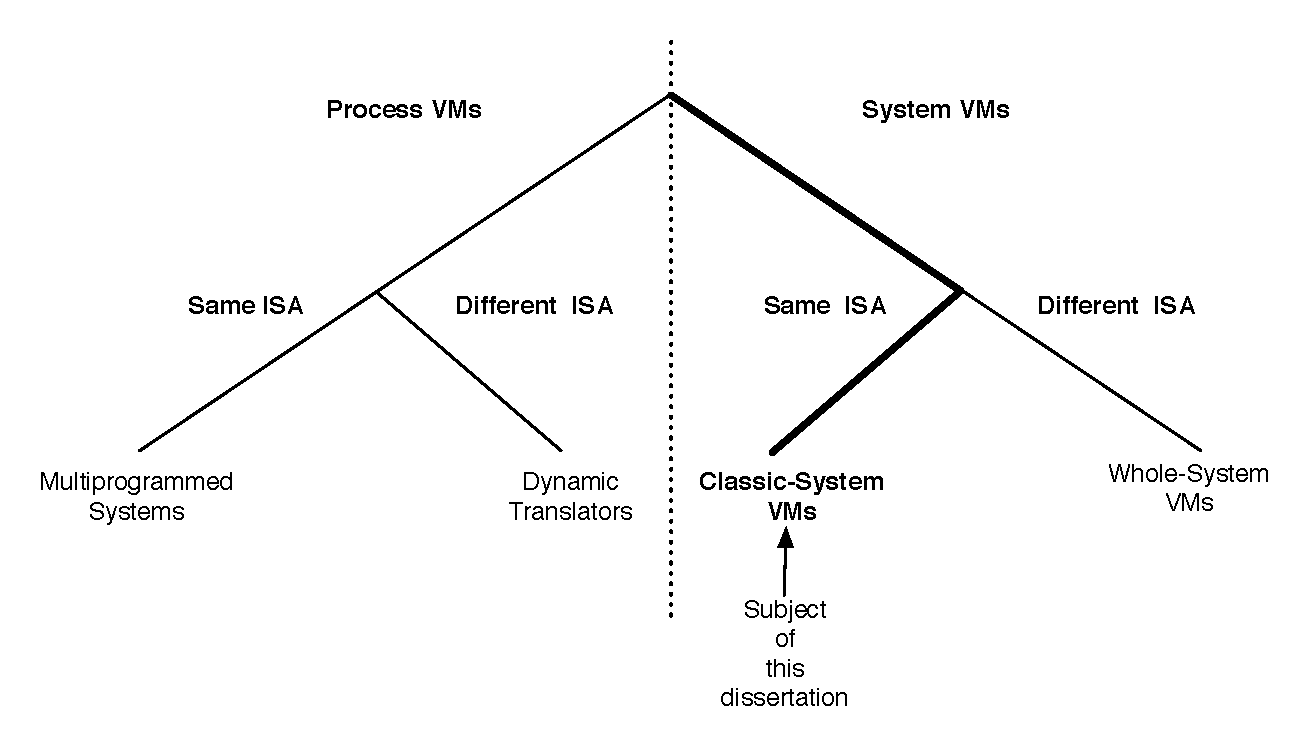
\includegraphics[width=0.7\textwidth]{chapter2/figures/taxonomy}
	\caption{A taxonomy of Virtual Machines. Classic-system VMs are the subject of study of this dissertation. Adapted from \cite{Smith2005}.}
	\label{fig:taxonomy}
\end{figure}


Interpretation and binary translation have different performance profiles \cite{Smith2005}. Interpretation has lower startup overhead but greater overhead for overall execution. On the other hand, binary translation has high initial overhead in order to translate the instructions for the first time. Thus, some VMs use both techniques combined with a heuristic to determine which source instruction blocks will be interpreted or translated. The best example of a process virtual machine is the Java Virtual Machine \cite{Lindholm1999}. Java is a high-level language (HLL) designed for portability. The Java compiler generates a portable intermediate ISA that can be emulated by the Java Virtual Machine (JVM) for different host ISAs. 

In system VMs, the virtualization software is often called a \emph{virtual machine monitor} (VMM) or simply \emph{hypervisor}. System VMs designed to support different ISAs need to emulate all software (OSs and applications). Thus, they are also called whole-system VMs. There are important applications for this kind of VM. For example, an ARM platform including the processor, memory and peripherals can be fully emulated on an Intel IA-32 processor. Thus, the designers can test their software without the target hardware. Additionally, a legacy software can be supported by newer platforms without requiring engineering work to port. An example of a system VM for different ISAs is the QEMU \cite{qemu}. QEMU is an open source application that can be used either as an emulator or virtualizer. As an emulator, it can run OSs and programs compiled for different ISAs. When used as a virtualizer, it can execute the guest OS code directly on the host CPU. Another example is Open Virtual Platforms (OVP)\footnote{http://www.ovpworld.org/} designed to accelerate embedded software development allowing hardware platforms to be described in C language. Thus, the designers can describe their custom platform, testing and debug their software without the real target. 

System VMs to the same ISA, also called classic-system VMs, were developed during the 1960s and they were the first application of virtual machines. At that time, mainframe computer systems were large and expensive. Thus, computers needed to be shared among users. Different users sometimes required different OSs creating the first practical application for virtualization. With the popularization of PCs, interest in classic-system VMs was lost. However, during the 1990s with the appearance of server farms, the classic-system virtualization became popular once again. In this case servers are shared among several users and VMs are a secure way of partitioning the user's software. Classic-system VMs have a lower performance impact when compared to whole-system VMs because the hardware directly executes the VM's instructions.

Recently, the interest in classic-system VMs for embedded systems has increased. However, classic-system VM as applied to server virtualization does not fit directly with ESs. Their intrinsic characteristics as discussed in Section \ref{section:es} motivated the study of new approaches for virtualization on ESs. Thus, the subject of this dissertation is classic-system VMs for embedded systems. Hereafter, the term virtual machine refers to classic-system VMs, unless otherwise noted. 


\subsection{Types of Hypervisors}
\label{subsection:hypertypes}
%procurar referencia para os termos type 1 e type 2.

Virtualizing software (VMM or hypervisor) can be divided into two different kinds called \emph{type 1} and \emph{type 2}. Figure \ref{fig:hyper_types} depicts both. Type 1 hypervisors are also called \emph{native} or \emph{bare-metal} hypervisors. The virtualization layer is implemented between the hardware and the guest OSs, i.e., there is no native OS executing in a system that adopts type 1 virtualization as shown in Figure \ref{fig:hyper_type1}. A representative type 1 hypervisor is Xen (see Section \ref{section:xen}). A type 2 hypervisor is implemented as a distinct software layer on top of an existing OS  (see Figure \ref{fig:hyper_type2}). From the point of view of the underlying OS, it is treated as a normal process and is subject to the same scheduler policies as other user and system processes. In this kind of virtualization, a guest OS can coexist along with the non-virtualized user processes. A representative type 2 hypervisor is KVM (see Section \ref{section:kvm}).

When a home/office user desires to utilize virtualization for some purpose, type 2 hypervisors are most popular. The type 2 hypervisor is installed as a user's application on the existing OS. This technique allows the user to execute a guest OS along with other user applications. Thus, the guest OS is competing with user applications for system resources, and it is submitted to the same host OS policies as any other process. In terms of memory requirements, type 1 hypervisors are more efficient than type 2 since there is not the overhead of the host OS. Additionally, the hypervisor has the freedom to control all system resources. The main application for type 1 hypervisors is to execute multiple OSs on the same computer, which makes it the perfect choice for server consolidation. 

\begin{figure}[!hbtp]
\centering
\subfigure[Type 1 hypervisor.]{
	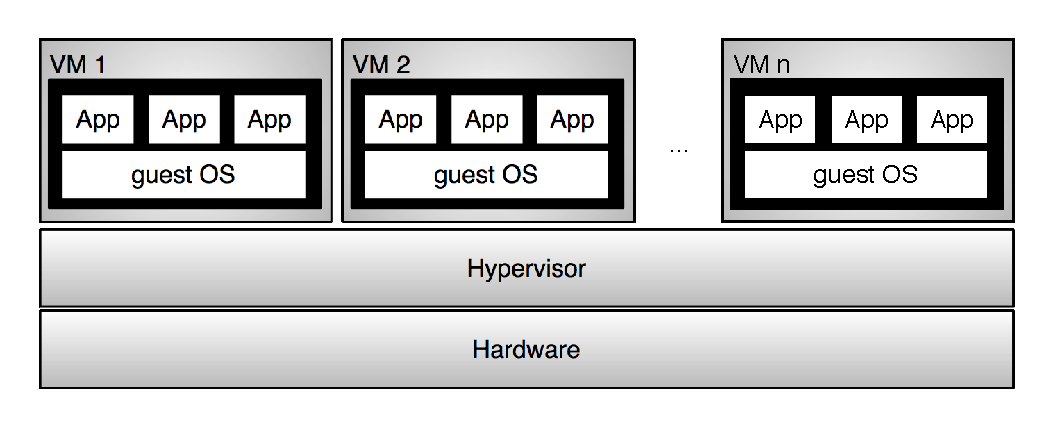
\includegraphics[width=.70\textwidth]{./chapter2/figures/hyper_type1}
	\label{fig:hyper_type1}}
\quad

\subfigure[Type 2 hypervisor.]{
	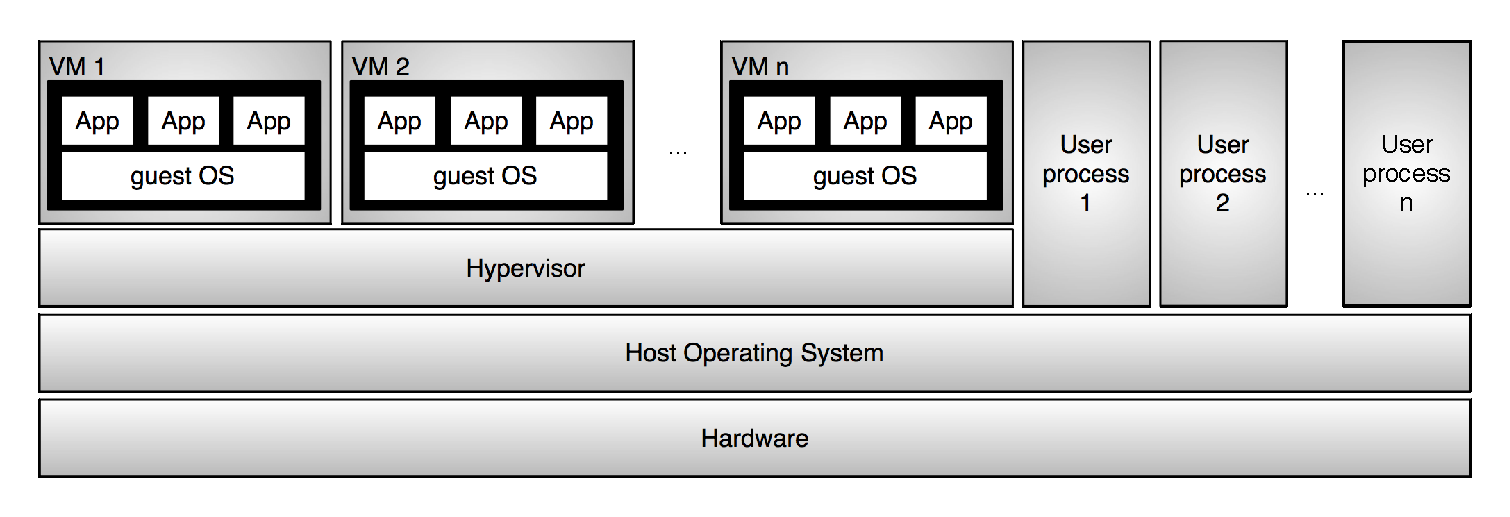
\includegraphics[width=.70\textwidth]{./chapter2/figures/hyper_type2}
	\label{fig:hyper_type2}}
\caption{Types of hypervisors.}
\label{fig:hyper_types}
\end{figure}

Type 1 and type 2 hypervisors are available for embedded virtualization. However, most type 2 hypervisors used in embedded virtualization were designed for desktop virtualization and adapted for embedded systems. As presented in the Chapter \ref{chapter:stateofart}, hypervisors designed specifically for embedded systems tend to implement the type 1 approach. Due to restrictions such as memory footprint and real-time constraints, the type 1 model fits embedded systems better. The virtualization model for ESs proposed in this dissertation depicts a type 1 hypervisor. 


\subsection{Requirements for Processor's Virtualization}
\label{subsection:vz-requirements}

The classic paper written by Popek and Goldberg \cite{Popek1974} formalizes the conditions for a processor architecture to be efficiently virtualized. Efficient  virtualization means  that a VM can be constructed over the processor's architecture without the necessity of modifying the guest OS. In order to understand their theorem, it is necessary to define the difference between control-sensitive, behavior-sensitive and privileged instructions. Control-sensitive instructions can change the configuration of the system's resources, while, behavior-sensitive instructions depend on the configuration of the resources. Instructions that are neither control-sensitive nor behavior-sensitive are termed innocuous \cite{Smith2005}. Moreover, instructions that trap the OS when executed in user mode are called privileged instructions. In a hypervisor, any instruction that attempts to change the configuration of the system's resources must be intercepted and emulated accordingly. This is possible when two requirements are accomplished: 

\begin{itemize}
  \item The instruction was executed in user-mode and;
  \item The control-sensitive and behavior-sensitive instructions are privileged instructions too. 
\end{itemize}  

The first requirement is easily accomplished executing the hypervisor in kernel-mode and the guest OS in user-mode. However, the second requirement relies on the processor's architecture. Thus, Popek and Goldberg stated their theorem:

\begin{thm}
"For any conventional processor a virtual hypervisor may be constructed if the set of sensitive instructions for that computer is a subset of the set of privileged instructions.
\end{thm}

Figure \ref{fig:sensitive_instr} depicts the theorem. In  Figure \ref{fig:sensitive_instr1} the control-sensitive instructions are not a subset of the privileged instructions, i.e., some of them can be executed in user-mode without trapping the hypervisor. This case violates Popek-Goldberg's theorem and cannot be efficiently virtualized.  On the other hand, Figure \ref{fig:sensitive_instr2} shows the control-sensitive instructions as a subset of the privileged instructions resulting in a processor that can be efficiently virtualized.

\begin{figure}[!hbtp]
\centering
\subfigure[Not efficiently virtualizable.]{
	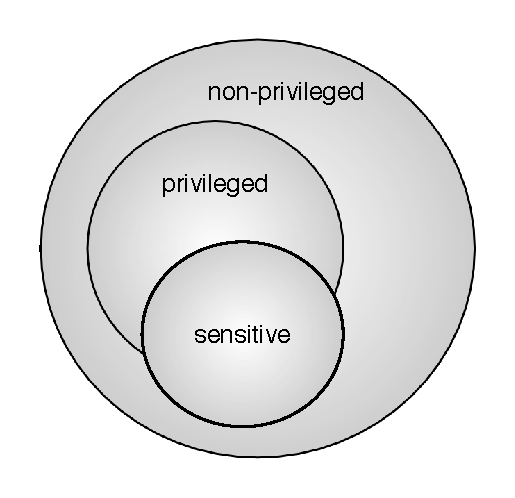
\includegraphics[width=.4\textwidth]{./chapter2/figures/sensitive_instr1}
	\label{fig:sensitive_instr1}}
\quad
\subfigure[Efficiently virtualizable.]{
	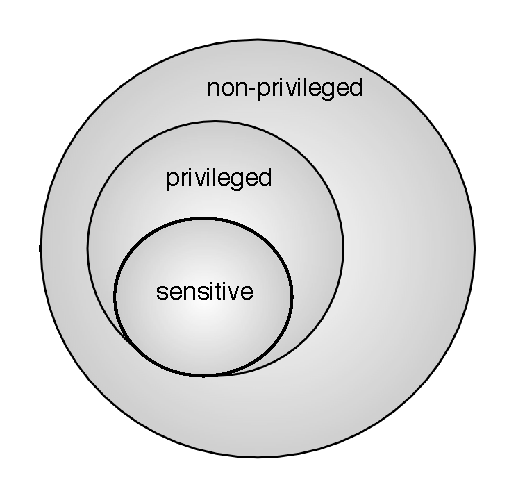
\includegraphics[width=.4\textwidth]{./chapter2/figures/sensitive_instr2}
	\label{fig:sensitive_instr2}}
\caption{Illustrating Popek and Goldbergs's Theorem. Adapted from \cite{Smith2005}.}
\label{fig:sensitive_instr}
\end{figure}

Para-virtualization (see Subsection \ref{subsection:paravirt}) can be applied when the processor's architecture is not compatible with the Popek-Goldberg theorem. Thus, allowing a hypervisor  implementation for that architecture. Alternatively, processors that support Popek-Goldberg’s theorem can be fully-virtualized (see Subsection \ref{subsection:fullvirt}). Section \ref{section:envirt} explains the difference between para-virtualization, full-virtualization and hardware-assisted virtualization. 


\section{Enabling Techniques and Technologies for Virtualization}
\label{section:envirt}

The evolution of virtualization technology has resulted in several different ap\-proach\-es. The variety of processor architectures and the appearance of new applications with different needs, has driven  techniques that can deliver virtualization on almost all devices. This section describes the three main techniques adopted for hypervisor implementation: para-virtualization (Subsection: \ref{subsection:paravirt}), full-virtualization (Subsection \ref{subsection:fullvirt}) and hardware-assisted virtualization (Subsection \ref{subsection:hardware-assisted}).  These techniques can be adopted separately or  through a hybrid approach, combining two or more of them. The virtualization model and the resulting hypervisor implementation, which is the subject of this work, are a combination of these three techniques.

\subsection{Para-virtualization}
\label{subsection:paravirt}

Hypervisors for processor architectures that do not fit Popek and Goldberg’s theorem, as explained in Subsection \ref{subsection:vz-requirements}, require different approaches. These architectures have control-sensitive instructions that do not trap the hypervisor. Therefore,  the hypervisor cannot avoid an application changing the processor's behavior. There are two ways to avoid this problem: dynamic binary translation or para-virtualization (PV). Hypervisors that perform dynamic binary translation need to read the VM's instruction prior to their execution in order to emulate the control-sensitive instructions that do not trap the hypervisor. Thus, causing a significant performance penalty when compared to PV. Para-virtualization is a technique that requires modifying and recompiling the guest OS prior to its installation in a VM. These modifications consist of substituting control-sensitive instructions or other OS parts, like the I/O subsystem, by hypercalls. However, for proprietary software or other situations where the source code is not available, the only alternative is dynamic binary translation.  

Hypercalls are services provided by the hypervisor and invoked from the guest OS. They are equivalent to system calls (syscalls) in an OS and Figure \ref{fig:syscall} describes their relationship. In operating systems, functions that can only be performed by the OS, like memory allocation or access to the file-system, result in calls to the OS. Similarly, functions that can only be performed by the hypervisor, such as the execution of control-sensitive instructions, can be converted to hypercalls. 

\begin{figure}[!hbtp]
	\centering
	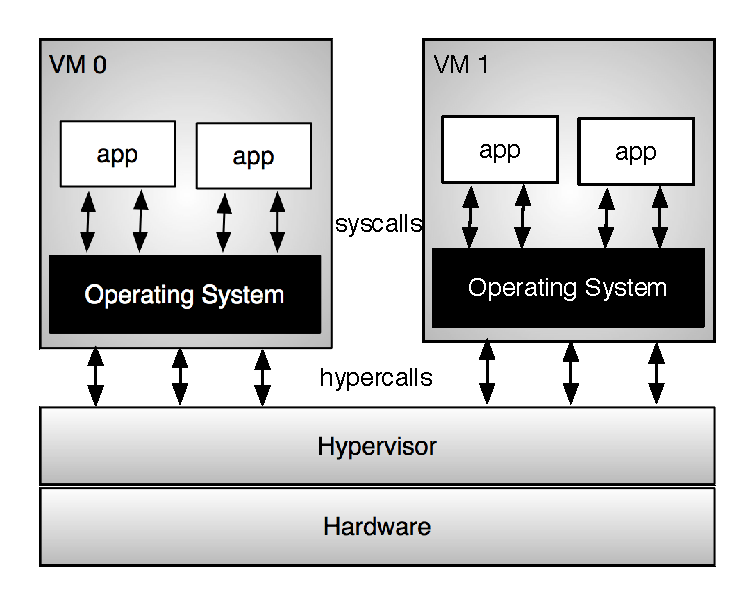
\includegraphics[width=.45\textwidth]{chapter2/figures/syscall}
	\caption{Relation between hypercalls on a virtualized system and syscalls on a typical operating system.}
	\label{fig:syscall}
\end{figure}

PV is not limited to processor architectures that cannot support Popek and Goldberg’s theorem. In fact, it can extend hypervisor capabilities. For example, PV can be used to implement communication between the VM and the hypervisor or inter-VM communication. Another application for PV is to improve performance, since fully-virtualized hypervisors have a performance issue. If the VM executes control-sensitive instructions constantly, it will result in an excessive number of traps to the hypervisor, impacting performance. Thus, the OS can be modified to substitute these instructions with hypercalls.  

The main limitation of para-virtualization is the engineering work needed to modify the OS to execute in a specific hypervisor. When utilized as a method to extend the capabilities of a virtualized platform, e.g., to support inter-VM communication, PV can be applied as a loadable module. Usually modern operating systems support kernel modules \cite{rubini2005}, i.e., executable code that can be dynamically loaded into an OS's kernel to add new functionalities. For example, an inter-VM communication module can be added without modifying the OS's source code. VirtIO \cite{Russell2008} is a effort to standardize the I/O interfaces for Linux hypervisors consisting of a set of Linux modules. However, para-virtualization used as a method to provide CPU virtualization, i.e., to avoid control-sensitive instructions, requires modifications to the OS's kernel. These modifications must be compatible with the hypervisor's requirements making them unique. 



\subsection{Full-virtualization}
\label{subsection:fullvirt}

The full-virtualization technique requires that the processor architecture fits with the Popek-Goldberg’s theorem to implement a virtual machine able to execute a guest OS without any modification. All privileged instructions must be emulated by the hypervisor. Full-virtualization allows the guest OS to be completely decoupled from the virtualization layer. Hence, the guest OS does not need to be modified to be virtualized. Unmodified guests are advantageous because they avoid additional engineering work. However, if the number of emulated privileged instructions are excessive, a fully-virtualized system can suffer from performance penalties. Due to this, para-virtualization was widely adopted in the first generation of embedded hypervisors.

Para-virtualization and full-virtualization can coexist in a combined approach. This approach consists of fully-virtualizing  the CPU and uses para-virtualization for certain peripherals or hypercalls for special services. For example, a network device may be para-virtualized to be shared among guest OSs or the hypervisor may implement a hypercall for a guest OS to change its execution priority. Additionally, the designers can implement hypercalls to substitute only instructions that generate an excessive number of traps and to use emulation for the remaining instructions. However, this requires prior study to determine what instructions must be substituted. 


\subsection{Hardware-assisted Virtualization}
\label{subsection:hardware-assisted}

This section offers a brief description of typical virtualization extensions. Dedicated hardware for virtualization can simplify hypervisor design and to improve performance and security. However, these advantages require additional hardware support increasing the processor complexity, cost and power consumption. These factors are critical for the ES market. Usually, the specification of virtualization extensions describes a full set of hardware features. However, this set of features must be flexible enough to allow for partial implementation. Thus, the processor's manufacturer can determine the level of hardware-assisted support based on the necessity of the market. For example,  limited hardware support may still allow for full-virtualization, but offers poor performance speed-up. In this scenario, the hypervisor must deal with the absence of features to support different processor models. Following is describe three important hardware features typically available in virtualization extensions sets. 

\subsubsection{Additional Privilege Levels}
\label{subsubsection2:privelege}

The typical para-virtualization approach on processors without proper virtualization support suffers from the inability to isolate the guest OSs’ kernel and user-space. The hypervisor is typically executed in kernel-mode and the entire guest OS is executed in user-mode. As a result, there is no memory isolation between the guest kernel and applications. Thus, a misbehavior or malicious application can disrupt the entire guest OS. A secondary effect is the excessive number of traps generated by the guest OS executing in user-space. This effect can be reduced with PV. 

Adding new privilege levels to the processor allows the guest OS to be executed in both kernel and user-modes, since the hypervisor is located in a higher privileged level. Figure \ref{fig:onion} shows the model of a processor implementing a third privilege level called supervisor.   Beyond allowing memory isolation inside the guest OS, the additional privilege level allows one to distinguish between user, kernel and supervisor exceptions. User exceptions, like system calls, can be handled directly by the guest OS kernel without the necessity to trap the hypervisor. Also, the hypervisor may control the accessibility of some hardware features, like configuration register or instructions, to the guest OS. Thus, the hypervisor may choose a policy of less intervention or a more controlled guest OS.

\begin{figure}[!hbtp]
	\centering
	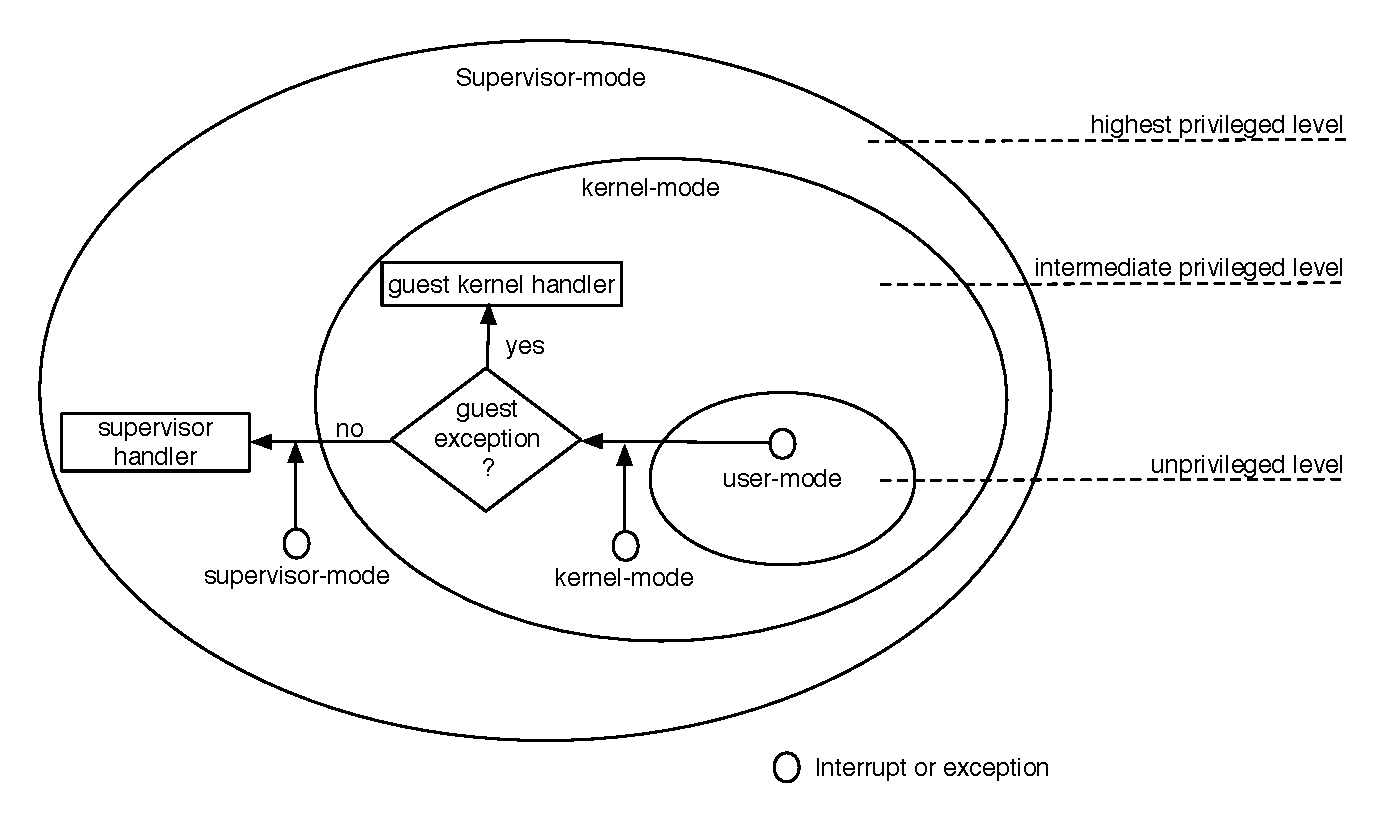
\includegraphics[width=0.6\textwidth]{chapter2/figures/onion}
	\caption{Supervisor privileged level for hypervisor execution.}
	\label{fig:onion}
\end{figure}


\subsubsection{2-Stage TLB Translation}
\label{subsection:tlb}

Processors targeting GPOSs rich in features must support a memory management unit (MMU) to provide a virtual memory mechanism. Thus, the OS can implement memory isolation between processes increasing software reliability and security. Translation look-aside buffer (TLB) is a common hardware construction to assist MMU, which works like a page table cache. High performance processors can automatically performs page walks in the page table when a TLB miss occurs, i.e., the target address is not found in TLB. However, simpler processors will trap the OS in this situation. Thus, the OS must handle a TLB exception to reconfigure the TLB cache. In a virtualized system, the hypervisor must virtualize the MMU keeping the guest OSes isolated from each other, which requires a second stage of address translation. Figure \ref{fig:ipa} shows the difference between virtual memory translation in a non-virtualized versus a virtualized system. In a non-virtualized system, the OS translates virtual addresses (VAs) to physical addresses (PAs) using its page table to configure the TLB. In a virtualized system, VAs are translated to intermediate physical addresses (IPAs), which must be managed by the hypervisor. Processors without the proper virtualization support require the hypervisor to implement a technique called shadow page tables that keeps the correct translation from IPA to PA. Figure \ref{fig:shadow} represents the difference between an OS page table and a hypervisor shadow page tables. When using this technique, the guest OS still manages its page tables, but it cannot configure the processor's TLB directly. The hypervisor handles the page faults reading the address mapping from the guest OS and creating its shadow page table. This second-stage address translation performed by software generates an excessive number of hypervisor exceptions, since, the TLB configuration involves privileged instructions. Again, the number of exceptions can be reduced using hypercalls. 

%\begin{figure}[!hbtp]
%	\centering
%	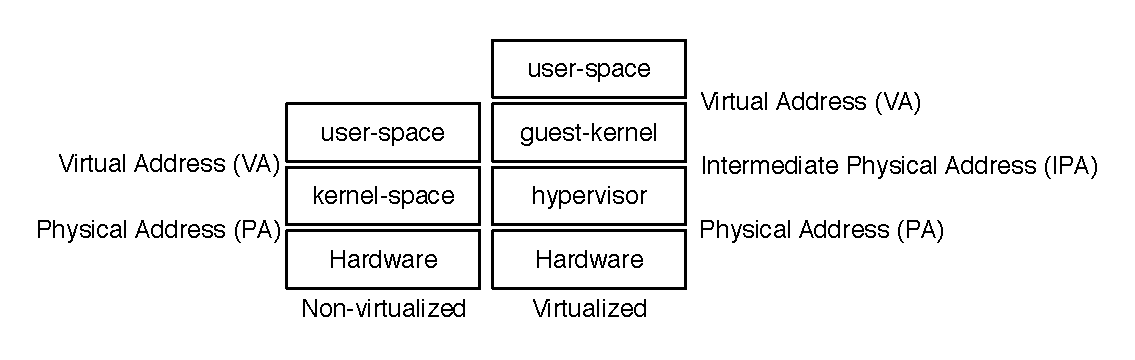
\includegraphics[width=0.9\textwidth]{chapter2/figures/ipa}
%	\caption{Non-virtualized versus virtualized virtual memory address translation.}
%	\label{fig:ipa}
%\end{figure}

\begin{figure}[!hbtp]
\centering
\subfigure[Non-virtualized versus virtualized virtual memory address translation.]{
    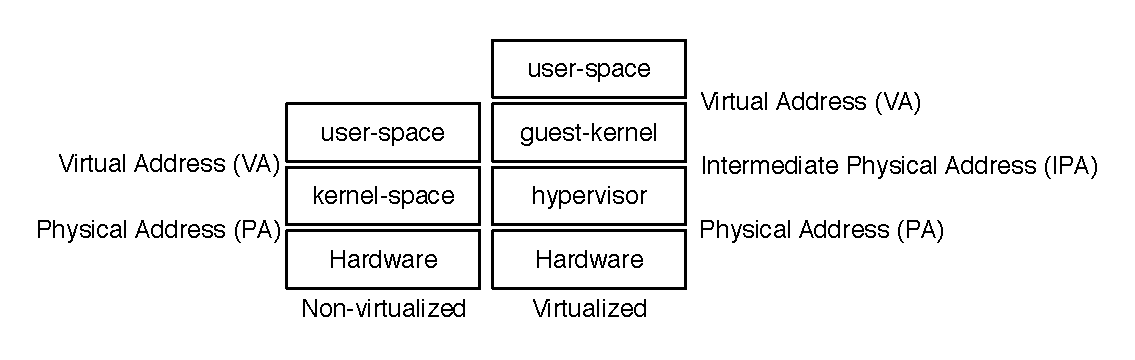
\includegraphics[width=.7\textwidth]{chapter2/figures/ipa}
    \label{fig:ipa}
}

\subfigure[OS page table versus hypervisor shadow page tables.]{
    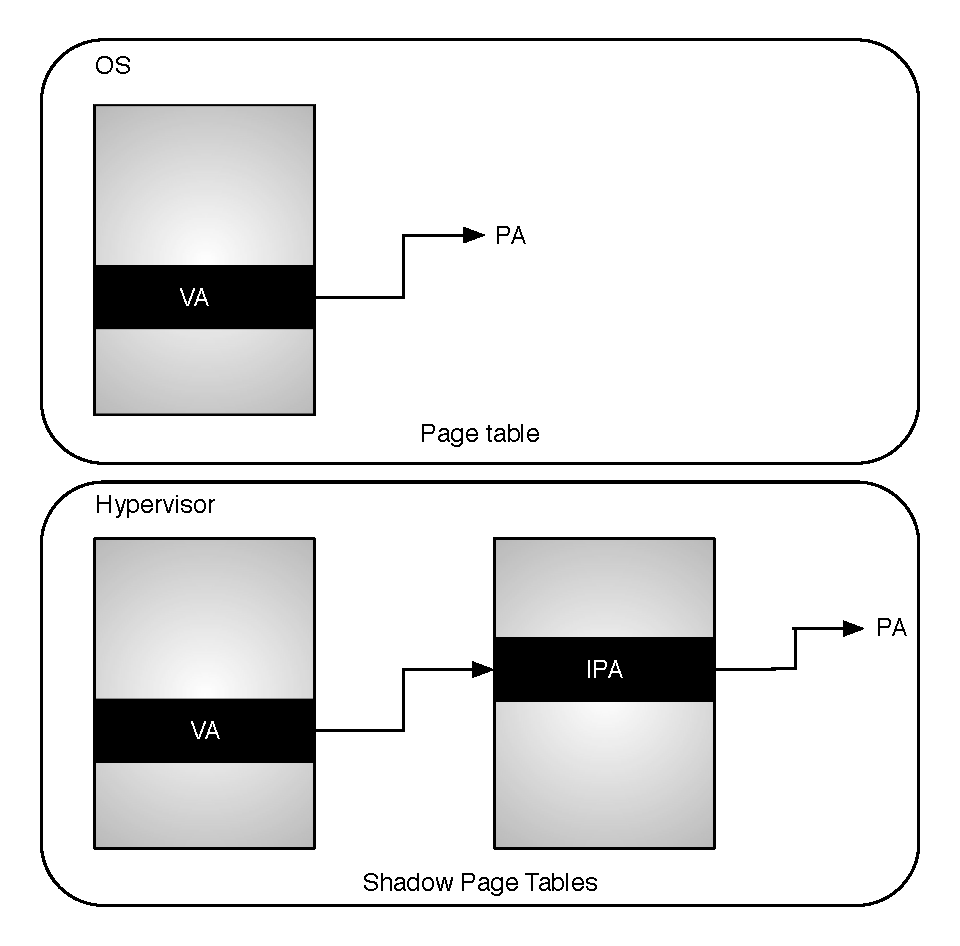
\includegraphics[width=.5\textwidth]{chapter2/figures/shadow-page-table}
    \label{fig:shadow}
}
\captionsetup{justification=centering}
\caption{Memory virtualization approaches in non-virtualized versus virtualized systems.}
%\label{}
\end{figure}


Current virtualization extensions for embedded processor families, like MIPS and ARM, implement a second-stage TLB translation in hardware. Essentially, the hardware performs the translation from IPA to PA without software intervention. The hypervisor still manages its page table mapping IPA to PA. However, the guest OS is allowed to configure directly the TLB. This is possible because the two TLB stages are configured from different processor modes. For example, the hypervisor (supervisor-mode) configures the second-stage TLB while the guest OS (kernel-mode) configures the first-stage TLB. The resulting PA is generated by the hardware combining both TLBs. This mechanism decreases the number of hypervisor exceptions drastically, since the guest OS directly manages  its TLB while decreasing the hypervisor complexity. 

%\begin{figure}[!hbtp]
%	\centering
%	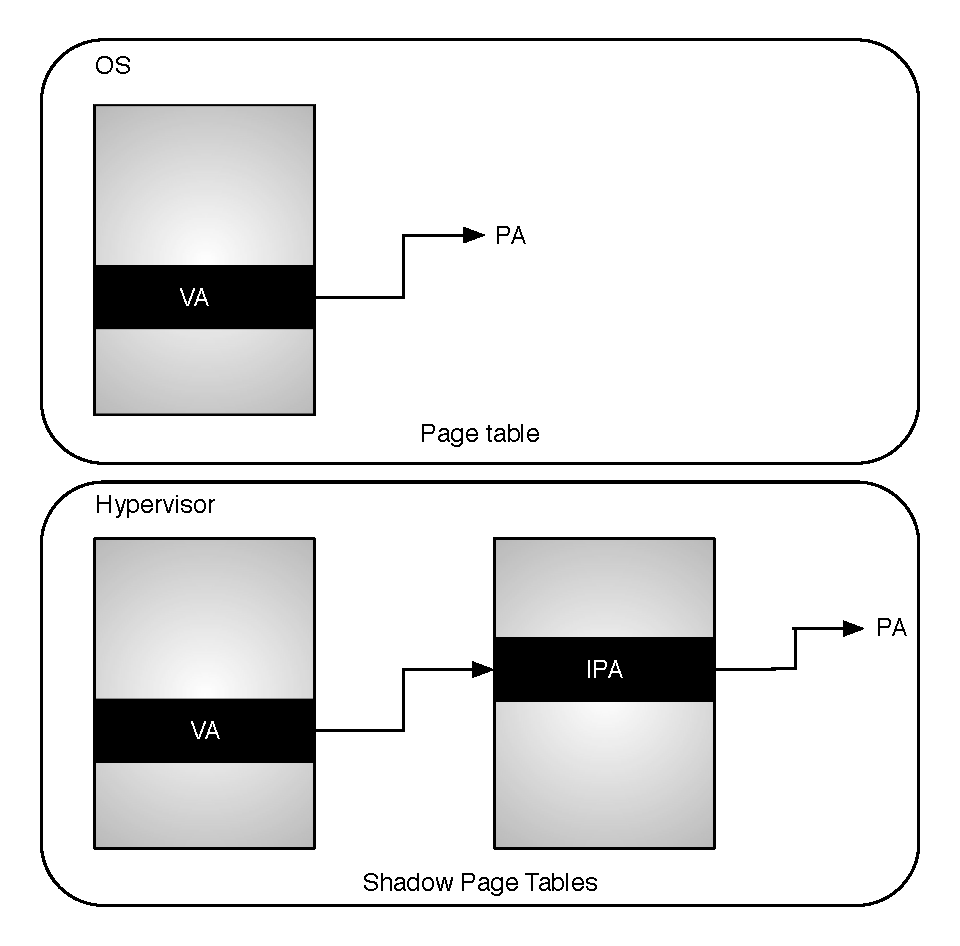
\includegraphics[width=0.4\textwidth]{chapter2/figures/shadow-page-table}
%	\caption{Page table versus shadow page table.}
%	\label{fig:shadow}
%\end{figure}



\subsubsection{Directly Mapped I/O}
\label{subsection:interrupt}

In some cases, it is desirable to map a hardware device directly to a guest OS, e.g., a serial port or a USB device could be directly handled by a guest OS. However, in processors without proper virtualization support, all interrupts are handled in kernel-mode forcing the hypervisor to handle all interrupt sources. This prevents an efficient implementation of a directly mapped I/O. 

One desired feature of a virtualization extension module is the capability of a hypervisor to map an interrupt source to a designed guest OS. For example, an interrupt used as system timer for guest OS scheduling purposes could be directly mapped, avoiding hypervisor intervention during the guest context-switch. Directly mapped devices require the hypervisor to configure an entry in its page table mapping the physical device address to the intermediate physical address (see Subsection \ref{subsection:tlb}) expected by the guest OS. Still, it must map the associated interrupts to the guest OS. Thus, the guest OS will receive  interrupts and read or write to the device without any hypervisor intervention. 


\subsection{I/O Virtualization}
%colocar referência para i/o overhead.
%referencia para IOMMU

There are different ways to manage I/O on a virtualized platform. On a platform without hardware-assisted virtualization, the hypervisor must implement device drivers for all peripherals in use, dealing directly with the system’s I/O. This technique is used in para-virtualized hypervisors. Thus, the device drivers at the operating system level are substituted by para-virtualized device drivers. Beyond to the disadvantage of modifying the OS's I/O subsystem to support para-virtualization, hypervisor intervention in I/O increases the virtualization overhead \cite{Waldspurger2012}. A directly mapped I/O can be used to improve the I/O performance on guest OSs, as explained in the Subsection \ref{subsection:hardware-assisted}. However, it lacks correct support for dynamic memory access (DMA) technique. DMA allows a peripheral to have direct access to the main memory. In a virtualized platform, the hypervisor re-maps the guest OS's memory addresses causing DMA devices to fail. Additionally, this is a security hole since a guest OS can use the DMA to transfer data to another guest OS's memory. Thus, the hypervisor must deny access to the guest OSs from the DMA controller, and to implement a para-virtualized mechanism to allow DMA to such systems. 

Modern processors with proper hardware support for virtualization implement a input–output memory management unit (IOMMU), as supported by the x86 family. IOMMU works similar to the processor's MMU (see Subsection \ref{subsection:tlb}). However, it translates memory accesses performed by devices instead of by the processor. Figure \ref{fig:iommu} compares IOMMU to the MMU. The IOMMU can solve the problem of memory re-mapping on virtualized platforms since the hypervisor can map the DMA addresses to the correct physical address. Additionally, it can avoid the security hole on DMA since it provides memory protection from peripheral read/write in a similar way that MMU provides spatial isolation.

\begin{figure}[!hbtp]
	\centering
	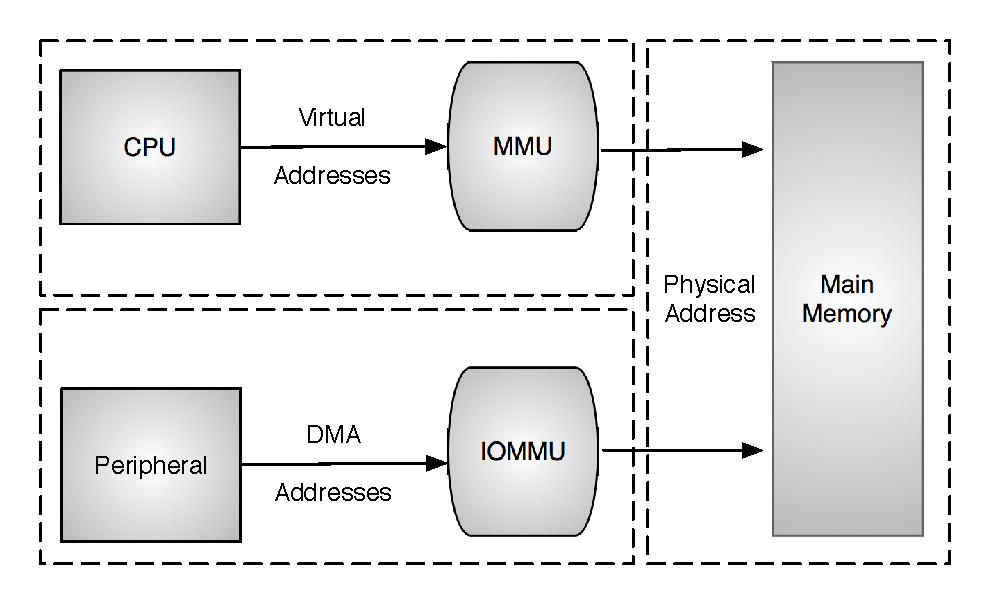
\includegraphics[width=0.55\textwidth]{chapter2/figures/IOMMU}
	\caption{Comparison of the IOMMU to the MMU.}
	\label{fig:iommu}
\end{figure}

Unfortunately, IOMMU is not present on all architectures of the current generation of hardware-assisted virtualization for embedded processors. For more details, Section \ref{section2:future} discusses the evolution of virtualization on embedded systems.


\section{Problems Caused by Virtualization}
\label{section:virt_challenges}

This section gives a brief introduction of two important problems faced in virtualized platforms: the hierarchical scheduling problem (Subsection \ref{subsection:twolayers}) and the lock the holder preemption problem (Subsection \ref{subsection:holder}). Chapter \ref{chapter:vtmodel} explains how the virtualization model proposed by this dissertation avoids this problems.

\subsection{The Hierarchical Scheduling Problem}
\label{subsection:twolayers}

As mentioned in the Subsection \ref{section:es}, real-time is a key feature in many ESs. Enabling real-time support on virtualized platforms causes the hierarchical scheduling problem, also known as two layers scheduling problem. A hypervisor schedules Virtual CPUs (VCPUs), and a guest RTOS executing in a VCPU schedules its processes or tasks. Even ensuring real-time characteristics at the VCPU level, it is difficult to ensure real-time execution to the tasks over the RTOS. However, if VM and hypervisor use proper real-time algorithms, the system can be modeled as a hierarchy of schedulers, and its real-time performance can be evaluated by using hierarchical scheduling analysis techniques \cite{cucinotta2009}.

One reason to use virtualization is to allow for the coexistence of different guest OSs designed for different purposes executing in the same system. For example, a \emph{general-purpose OS} (GPOS) executing along with a legacy RTOS. However, different OSs have different characteristics, e.g., RTOSs privileges real-time over throughput performance. A hypervisor for ESs must be flexible enough to deal with these conflicting characteristics. Thus, more effective approaches should be taken to deal with the two layer scheduling problem. 

Some authors, e.g., Kiszka et al. \cite{kiszka2009}, propose the implementation of hypercalls to allow the guest OS to inform to the hypervisor of its time constraints. Other approach is the use of compositional scheduling as proposed by Lee et al. \cite{Lee2012}. Additionally, an alternative adopted by this dissertation is to perform the scheduling of real-time tasks directly by the hypervisor, i.e., avoiding the two layer scheduling problem and performing a strong temporal separation between general-purpose guest OSs and real-time entities.


\subsection{Lock Holder Preemption Problem}
\label{subsection:holder}

The Lock Holder Preemption (LHP) problem in a virtualized environment happens if a guest OS executing in a SMP configuration is preempted while its kernel is holding a spinlock. Spinlocks are a synchronization primitive widely used in OS's kernels. With spinlocks, a thread waiting to acquire a lock will wait actively monitoring the lock \cite{mitake2012}. As this lock remains, any other VCPU from the same guest trying to acquire this lock will have to wait. Spinlocks imply active waiting, thus, the CPU time is wasted resulting in serious performance and real-time degradation. The LHP problem is possible even if two or more VCPUs execute on a single physical CPU concurrently.

Several approaches were proposed to deal with the LHP problem. The VMWare hypervisor\footnote{http://www.vmware.com/} employs the co-scheduling technique \cite{ousterhout1982}, consisting of a scheduler that tries to execute processes communicating with each other in the same time slice, thus, reducing the chances of blocking. Uhlig et. al. \cite{uhlig2004} proposed a full-virtualized and a para-virtualized technique to deal with the problem. In the full-virtualized technique, the authors consider that the spinlocks are always acquired and released in kernel mode. Thus, the hypervisor never preempts the guest OS when executing in kernel mode, avoiding the LHP problem. Their para-virtualization technique consists of a hypercall to be invoked when entering in spinlock and another hypercall to be invoked when leaving the lock. Thus, the hypervisor knows when a VCPU is in a spinlock and should not preempt it. 

In ES, the main consequence of the LHP problem is the impact in real-time responsiveness. Thus, the LHP should be carefully considered when designing a virtualized ES.


\section{Virtualization for Embedded Systems}
\label{section:ev}

Virtualization is a widespread technology for enterprise and workstation applications, but, it is a relatively new concept in the ES area. The importance of virtualization for ESs is due to its ability to address some of the growing challenges in this area, e.g., the increasing software complexity and time-to-market. One advantage of virtualization is its ability to support heterogeneous operating-system environments to address conflicting requirements such as high level APIs, real-time support or legacy software. The architectural abstraction offered by virtualization allows for migration of multicore guest OSs to virtualized single core systems essentially without modification. Security is another important motivation, since, virtualization can enable a strong spatial separation between the guest OSs \cite{HeiserRole}. 
Virtualization as deployed in the enterprise environment cannot be directly used in ESs. Although ESs are starting to implement some features of general-purpose systems, some differences remain. ESs still present critical real-time constraints and frequently have resource constraints, such as reduced battery capacity, memory and processing power. Thus, virtualization in the ES world is a different challenge than that faced in the enterprise environment. To distinguish server virtualization from embedded system virtualization, the term embedded virtualization is used. Additionally, in this dissertation the term virtualization refers to embedded visualization unless stated otherwise.

This dissertation focuses on embedded systems that require large software stacks to implement their functionalities. These systems can use virtualization to meet these requirements. In addition, the proposed virtualization techniques presented in this dissertation can be used to improve real-time responsiveness and increase security on ESs. Some examples of ES candidates are customer electronics (CE) like smart phones, tablets, set-up box among others. Moreover, enterprise and industrial electronic devices such as network devices (routers and switches) may apply embedded virtualization. Recently, virtualization for IoT devices emerged as a trend. The main advantage of virtualization on IoT is security. Hypervisors can provide memory isolation between applications and implement a Root of Trust software base, which means an environment where the hypervisor guarantees the authenticity of the virtual machines. 

\section{Past, Present and Future of Embedded Virtualization}
\label{section2:future}

Roughly ten years ago, virtualization started to move to the ESs field. At that moment, embedded virtualization was ruled by hypervisors that adopted para-virtualization to overcome the performance issues of full-virtualization. Though some popular hypervisors used for server computing were adapted for embedded systems, other hypervisors were developed from scratch. Some of these hypervisors are still in use, and they will be discussed in Chapter \ref{chapter:stateofart}. These hypervisors were especially designed to deliver virtualization in embedded systems, but in a lightweight way, and implement techniques to improve the real-time responsiveness along with memory separation. 

With the advance of the semiconductors and their decreasing cost, it is possible to implement hardware support for virtualization on embedded processors affordably. The first embedded processors with hardware-assisted virtualization emerged around five years ago. The possibility of implementing full-virtualization without the performance penalties of the past motivated the appearance of newer hypervisors. The current stage of embedded virtualization allows full-virtualization of the CPU combined with para-virtualized I/O. Thus, hybrid hypervisors combine full and para-virtualization. In a few years, proper support for IOMMU on embedded processors will allow for high performance communication between guests using the DMA hardware. 

In the next five years, virtualization will increasingly be used in embedded systems \cite{security-prpl}. Virtualization will not be restricted to powerful embedded devices, but will also be used in IoT devices, primarily motivated by security concerns. Thus, embedded hypervisors will need to execute in devices with extreme hardware restrictions. Small footprint and lightweight execution will still be important.




\chapter{\label{chapter:stateofart}State-of-the-Art in Embedded Virtualization}

This section describes the current status of embedded virtualization. As shown in Chapter \ref{chapter:background}, hypervisors designed for general purpose virtualization cannot be directly adopted for ES. However, this chapter starts by showing well-known hypervisors widely used for cloud computing. They present larger footprints and overheads than hypervisors that are specially designed for embedded systems. Several authors have dedicated their work to adapting them for ES. The chapter is divided into the following sections:  Subsection \ref{section:xen} presents the architecture and proposals based on the Xen hypervisor. Xen was designed for enterprise appliances. Therefore, there are ports for embedded devices and special support for real-time. Subsection \ref{subsection:kvmproposals} presents proposals based on KVM (Kernel-Based Virtual Machine), a type 2 hypervisor, which was ported for the ARM architecture. The remaining hypervisors that will be presented were developed for  ES. Section \ref{section:spumone} describes the SPUMONE hypervisor. Section \ref{section:XtratuM} presents XtratuM, a hypervisor for safety critical systems. Section \ref{section:l4} presents three different embedded hypervisors based on the L4 microkernel family: OKL4, L4/Fiasco, PikeOS and Mini-Nova. Section \ref{section:mhyper} presents the M-Hypevisor. Section \ref{section:xvisor} shows the XVisor embedded hypervisor. A comparative study between the hypervisors is presented in Section \ref{section:comparative}. Section \ref{section:rtlinux} explains how the RT-Linux patch modifies the Linux kernel and how it is similar to virtualization. Finally, Section \ref{section3:considerations} concludes this chapter. 


\section{The Xen Hypervisor}
\label{section:xen}

Xen is an open-source type 1 hypervisor that has been developed over the last 13 years \cite{xen2003}. Today, Xen is used for different commercial and open-source projects, such as: server virtualization, desktop virtualization, security and embedded applications. Additionally, Xen supports the largest clouds in production today\footnote{http://www.xenproject.org/}. Initially developed for desktop or server application, it was modified to be embedded, especially for ARM processors.

\subsection{Xen's Architecture}
\label{subsubsection:xenarch}

Figure \ref{fig:xenarch} depicts Xen's architecture. Xen is responsible for handling CPU, memory, interrupts and scheduling the VMs. Xen is a type 1 hypervisor, thus, it interacts directly with the hardware and the VMs executes over it. A running instance on a VM in Xen is called domain or guest. There is a special domain, called \emph{Domain 0} (Dom0), that is responsible for I/O and also contains a stack to manage the VM’s creation, destruction and configuration, called \emph{Toolstack}. 


\begin{figure}[!hbtp]
\centering
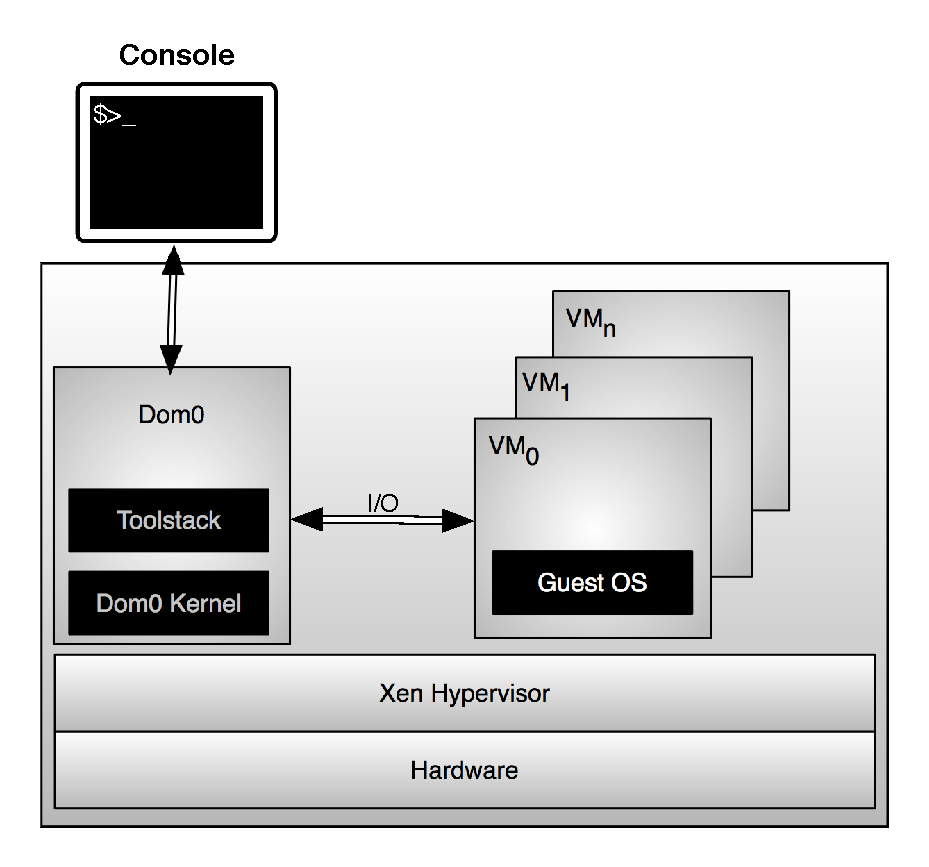
\includegraphics[width=.45\textwidth]{./chapter3/figures/xenarch}
\caption{Xen's Architecture. Adapted from \cite{xen2003}.}
\label{fig:xenarch}
\end{figure}

The Xen hypervisor has less than 150,000 lines of code and a footprint around 600KB. However, the footprint can variate with different compilers and compilation flags. Xen does not implement I/O functions such as networking or storage itself. Instead, I/O functionality is accomplished by the Dom0. Dom0 has special privileges to access the hardware directly and it is responsible for handling the I/O for all VMs. Thus, if a VM needs an I/O function it must interact with Dom0, which will execute the transaction with the hardware. Additionally, the Dom0 implements the Toolstack, which exposes an interface composed of the command line and graphical interface, as well as interacts with cloud APIs like OpenStack \cite{openstack} for configuration purposes.

The Xen architecture requires that the guests are modified (patched), since all I/O are redirected to Dom0. Essentially, Xen was designed to be a para-virtualized hypervisor. Therefore, this approach prevents  unmodified guest OSs be virtualized on top of Xen. Thus, proprietary OSs like Microsoft Windows can not be virtualized. Aiming to overcome this limitation, Xen implements the hardware-assisted virtualization (HVM) that uses virtualization extensions from the CPU, like Intel VT or AMD-V. Xen does not deal with I/O directly, thus, it needs to use the Qemu \cite{qemu} to emulate BIOS, IDE disk controller, VGA graphics adapter among others devices. This allows for Xen to perform full-virtualization. However, the device emulation causes a performance issue and fully-virtualized guests over Xen are usually slower than the para-virtualized ones. Nonetheless, Xen provides a technique to avoid the performance issue when using HVM, called PV on HVM. This technique consists in to combine para-virtualization and full-virtualization. Thus, para-virtual device drivers are installed in the guest OS to bypass the emulation for storage and network I/O. CPU and memory virtualization continues to be performed by hardware support. This allows for performance improvement for guest proprietary or even open source OSs. However, it requires the implementation of para-virtual device drivers to the guest OSs. Both PV and HVM guests can coexist on a single Xen system.

\subsection{The Xen Scheduling Algorithm}
\label{subsubsection:xensch}

An important component of a hypervisor is the scheduler. The default Xen's scheduler is called Credit Scheduler \cite{Ding2014}. Xen implements two other scheduling algorithms: the Simple Earliest Deadline First (SEDF) \cite{sedf} and the Borrowed Virtual Time (BVT) \cite{Duda:1999}. Although at the present time both algorithms are available, they are marked as deprecated and probably they will be removed from the Xen's source code. Nevertheless, several works still rely on SEDF to improve real-time on XEN. Thus, just the Credit Scheduler and the SEDF will be discussed. 

In the Credit Scheduler, each domain has two special attributes: weight and cap. The weight determines the proportional fair share of CPU resource. For example, a domain with weight of 1024 will get the CPU two times more than a domain with weight of 512. The weight values range from 1 to 65535 and the default is 256. The cap is an optional parameter used to determine the amount of CPU that a domain will be able to consume, even if the host system has idle CPU cycles. The cap is expressed as a percentage of one physical CPU. For example, a cap of 0.5 means that the domain can take up to 50\% of CPU time, 1 means the domain can take upto 100\% of the CPU time and 2 means the domain can take upto 100\% of two CPUs' time. When cap is 0 means there is no limit for CPU usage.  Credit scheduler keeps a local queue of runnable VCPUs by physical CPU ordered by priority. When a VCPU is scheduled, the algorithm computes how much time (credits) was consumed and subtracts from the total time reserved for it. If the VPCU exceeds its available credits it is in "over" status, otherwise, it is in "under" status. Once in over status, the VCPU needs to wait for the next period to execute again. By default, the scheduler quantum is 10ms and the VCPU credits are recomputed each 30ms. In a SMP platform, when a CPU does not find a VCPU in under status in its local queue, it looks on other CPU queues for one. This is called SMP load balancing and it guarantees that there is not an idle CPU when there are runnable VPCUs in the system.

The SEDF scheduler allows to allocate processing resources for each domain according to period, deadline (the time when the period ends) and capacity (the amount of processing time reserved to the domain in a period). In fact, the algorithm guarantees that a domain will be executed for the amount of time given by its capacity on each time interval given by its period \cite{Ongaro2008}. The algorithm keeps the deadline for each domain and the amount of processing remaining to be done before the deadline. The domains are sorted in the execution queue according to their deadlines. An interesting effect of this algorithm is that when a domain consumes processing time, its deadline will be moved forward. Thus, I/O-intensive domains that consume little processing time will typically have earlier deadlines, which means higher priority over CPU-intensive domains. This is advantageous to environments that combine CPU and I/O intensive domains. The main disadvantage of the SEDF algorithm is to keep local queues organized by CPU on multicore processors preventing VCPU migration across multiple cores and avoiding dynamic workload balance. Nevertheless, it was made obsolete because with Credit scheduler is possible to improve scheduling performance on multiprocessors.


\subsection{Xen-Based Proposals}
\label{subsubsection:xenproposals}

The proposals to improve real-time responsiveness on Xen hypervisor are typically based on two different approaches: a) improving the Xen's scheduler real-time responsiveness, or; b) dealing with the hierarchical scheduling problem. The first approach typically tries to improve the real-time scheduler responsiveness by applying different scheduling algorithms or non-intrusive techniques to monitor the guest’s behavior. Nevertheless, such approaches generally do not consider the hierarchical scheduling problem. The second approach uses theoretical research on hierarchical real-time scheduling or intrusive techniques that require modifications inside of  the guest OSs.

\subsubsection{Improving The Scheduler's Real-time Responsiveness}

Ongaro et al. \cite{Ongaro2008} studied the performance impact on the Xen hypervisor when multiple guests with different workloads (CPU-intensive, I/O-intensive and latency-sensitive) run concurrently. The results led to some optimization proposals, including disabling preemption for Dom0 and sorting the scheduler run queue based on the remaining credits  to give priority to I/O-intensive domains. These optimizations were focused on improving the I/O performance, nevertheless, the authors claim that it impacts latency positively. Finally, their study showed that latency-sensitive applications will perform better when not combined in the same domain with CPU-intensive applications. Instead, latency-sensitive applications should be placed within their own domain. 

Lee et al. \cite{Lee2010} introduced the laxity concept enhancing the soft real-time performance of the Xen Credit scheduler. Each domain has an attribute named laxity used to define the position where its VCPUs will be inserted in the scheduler's run queue. In other words, it is possible to use laxity to determine the maximum desired latency for a real-time domain, because when a VCPU is inserted into the run queue, it is inserted where its deadline is expected to be met. 

Masrur et al. \cite{Masrur2010} implemented a new scheduler for Xen based on the SEDF scheduler aiming to improve its worst-case response time, named  \emph{Priority-based scheduling plus SEDF} (PSEDF). The major difference is that PSEDF implements the concept of real-time domains (domRT), where, a domRT has scheduling priority over non real-time ones (domU). When several domRTs coexist at the same Xen instance, priorities must be defined between them. The domUs continue to be scheduled with the default SEDF. The resulting scheduler allows safety-critical applications (e.g. airbag control and brake system) to be run on the same hardware with general-purpose applications (e.g. navigation and multimedia). The main drawback of the authors’ technique is that a domRT can just contain a single real-time application to avoid the hierarchical scheduling problem.

Hu et al. \cite{Hu2010} proposed a technique to improve the I/O performance of Xen on multicore processors. Their technique take advantage of the fact that traditional hypervisor schedulers, including Xen, focus on sharing the processor's resources fairly among domains, while, the scheduling of I/O resources is treated as a secondary problem. This seriously impacts on the performance of applications that execute I/O-intensive tasks, like network or storage. The authors’ technique consists of implementing  a scheduler for multicore dynamic partitioning, where, the processor cores are divided into three specialized subsets with different scheduling strategies. The subset called driver core host only the dom0, i.e, the dom0 is bounded to a physical core and never is scheduled. The fast-tick cores subset handles I/O events and its scheduler employs small time slices to ensure fast response to I/O events. Finally, the general cores subset is used for computation-intensive workloads. Their approach increases I/O performance, although, it degrades the performance for CPU-intensive applications.

Huacai et al. \cite{huacai2010} proposed improvements to Xen's Credit scheduler from the real-time perspective to guarantee audio performance (avoiding human-sensible glitches) in virtualized environments. Their strategy consist of three approaches: flexible time slices, real-time priority adjustment and adaptive audio-aware. The Credit scheduler was modified to allow flexible time slices, i.e, the scheduler restriction of fixed time slices or quantum of 10ms (see Subsection \ref{subsubsection:xensch}) was removed allowing different time slice lengths. For example, a real-time domain may receive 1ms time slice and a non real-time may receive the default time slice (10ms).  The real-time priority adjustment promotes a domain from non real-time to real-time when the user plays audio. The adaptive audio-aware algorithm is used to detect when the user starts/stops the audio player given to it a higher priority. 

Credit scheduler was designed to be efficient with computation intensive workloads. However, I/O-intensive tasks suffer from latency issues. To minimize this problem, Zeng et al. \cite{zeng2013} enhanced performance to the I/O latency-sensitive applications minimizing the system response time by balancing the VCPUs with BOOST priority in multi-core systems. BOOST is an additional priority level of the Credit scheduler, which allows a VCPU to preempt a running VCPU in under state. The results showed that their proposal can improve the response time for latency-sensitive applications without having adverse impact on compute-intensive applications. 
 
Cheng et al. \cite{cheng2015} optimized the Xen's scheduler for soft real-time applications. They introduced a new priority level marking high priority VMs as real-time domains. Additionally, their strategy includes management of the physical CPU's queue, limiting the number of real-time domains to guarantee to meet the scheduling requirements, and pinning VCPUs to physical CPUs to reduce the performance impact caused by VCPU migration. The authors evaluated their solution using IP telephony workloads for soft real-time applications. The results compared to Credit scheduler and RT-Xen showed that their purpose achieves best performance and maintains a fairer scheduling in the meantime.

\subsubsection{Dealing With The Hierarchical Scheduling Problem}

Masrur et al. \cite{Masrur2011} proposed the design of a scheduler to deal with the hierarchical scheduling problem targeting automotive applications. The authors consider that all domains schedule their applications using the deadline-monotonic scheduler algorithm. On the other hand, the hypervisor utilizes the rate-monotonic scheduler algorithm \cite{Buttazzo2005} \cite{brun2015} for VCPU scheduling. Thus, they proposed a method to determine optimum time slices and periods for each VM in order to maintain their time constraints. The proposed scheme was validated using the Xen hypervisor. Their solution solves the hierarchical scheduling problem without hypercalls between the VM and hypervisor, although the Xen's default scheduler algorithm must be modified to accommodate the rate-monotonic algorithm. 

The RT-Xen project \cite{sisu2011} implements a hierarchical scheduling architecture based on fixed-priority scheduling focused on soft real-time applications for single-core processors. It considered four fixed-priority scheduling policies for the RT-Xen scheduler: Deferrable Server \cite{strosnider1995}, Sporadic Server \cite{sprunt1989}, Periodic Server and Polling Server \cite{sha:1986}. The four scheduling policies were implemented and compared to Xen's Credit Scheduler and SEDF schedulers. The experiments was conducted using a modified kernel Linux implementing the rate-monotonic scheduling algorithm. The results show that RT-Xen presents an acceptable soft real-time performance. The Deferrable Server presented the best results, while the Periodic Server suffered from a high number of missed deadlines in overloaded situations. Recently, it was released the RT-Xen 2.0 \cite{sisu2014} supporting multi-core processors and up to eight combinations of real-time VM scheduling policies. Moreover, it supports a range of interfaces for compositional scheduling, which enables designers to calculate and specify the resource demands of VMs to the underlying RT-Xen 2.0 scheduler. 

Lee et al. \cite{Lee2012} proposed a Compositional Scheduling Architecture (CSA) that enables timing isolation among VMs and supports timing guarantees for real-time tasks running on each VM. The CSA supports a broad range of real-time scheduling algorithm at the hypervisor level, and it was implemented extending the original RT-Xen interfaces. The authors presented an extensive evaluation to demonstrate the utility and effectiveness of CSA in optimizing real-time performance. The results using both synthetic and avionics workloads showed significant improvements regarding response time.

Yoo et al. \cite{seehwan2014} studied the schedulability in VMs considering the quantization overhead caused by the Xen's scheduler. Quantization overhead comes from tick-based scheduling of Xen-ARM, which requires integer presentation of scheduling period and execution slice. To minimize the quantization overhead they proposed a new algorithm to provide accurate and efficient parametrization of real-time VMs. Next, they presented an inter-VM schedulability test to the real-time VMs. Their proposal was evaluated on an ARM platform using a RTOS. Their experiments showed that is possible to guarantee the deadline for real-time tasks scheduled in a hierarchical fashion. However, the SEDF scheduler must be used as Xen's scheduler. Moreover, their work does not cover the I/O, since it is complex in Xen and requires a separate investigation. 

\subsubsection{Other Proposals}

Avanzini et al. \cite{avanzini2015} proposed the integration of the ERIKA OS\footnote{http://erika.tuxfamily.org/drupal/} and the Linux on a dual-core processor through Xen. ERIKA OS is an open-source, low-footprint and real-time operating system certificated for automotive applications. Their system configuration consisted in the Linux as dom0 and ERIKA OS as domU. The system was prototyped on a cubieboard2\footnote{http://cubieboard.org/}, an ARMv7 with virtualization extensions. In their proposed setup, each of the domains runs on a dedicated core, assigned statically by the hypervisor. Linux is the control domain, thus performing the Xen toolstack. Moreover, it must grant to ERIKA access to any I/O-memory range needed. Their approach provides an improved temporal isolation of concurrent operating systems. The main drawback is to keep the guests on dedicated cores not allowing load-balancing. 

\section{KVM Hypervisor}
\label{section:kvm}

The Kernel-based Virtual Machine (KVM) is a type 2 hypervisor designed to be a kernel-resident virtualization infrastructure, meaning it is totally integrated with the Linux Kernel since the 2.6.20 release. KVM is implemented as a Linux kernel module providing full-virtualization when hardware-assisted virtualization is supported, otherwise it provides para-virtualization. It supports SMP hosts and guests and enterprise level features like live migration\footnote{http://www.ibm.com/developerworks/library/l-hypervisor/}, which is the ability to move guest OSs between physical servers.

\subsection{KVM's Architecture}
\label{subsection:kvmarch}

KVM's architecture is shown in Figure \ref{fig:kvmarch}. It is composed of two main components: the KVM-loadable module that manages the virtualization hardware and exposes a configuration interface through the /dev file system; and a modified version of Qemu, called qemu-kvm, used to provide platform peripheral emulation. 

\begin{figure}[hbtp]
\centering
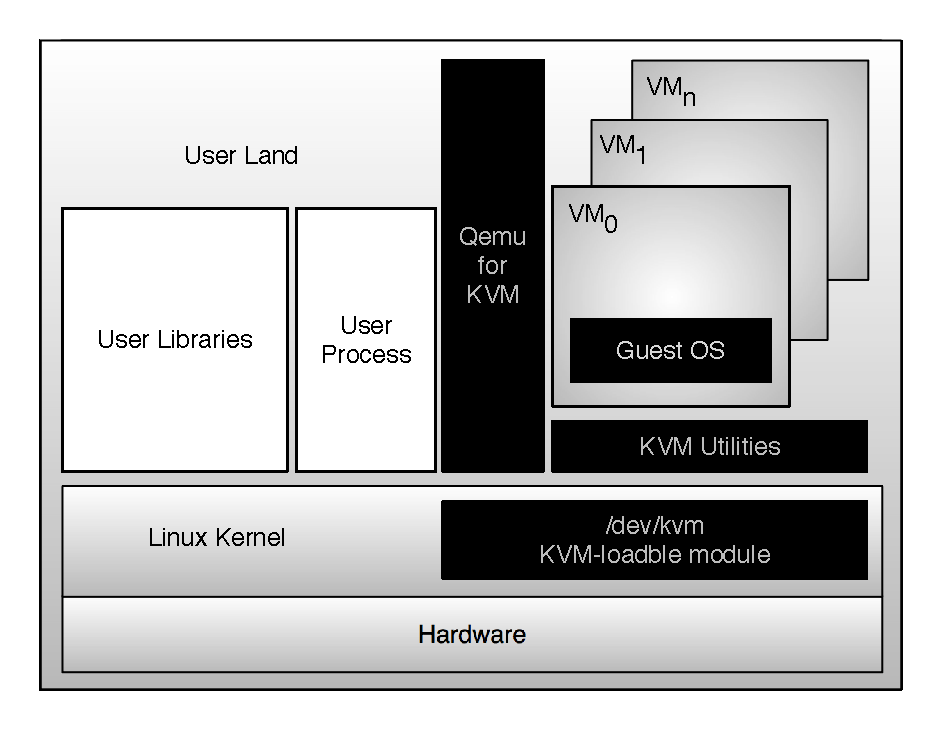
\includegraphics[width=.45\textwidth]{./chapter3/figures/kvmarch}
\caption{KVM's Architecture.}
\label{fig:kvmarch}
\end{figure}

A utility called kvm is used in user land to boot a guest OS in KVM. Once booted, the guest becomes a process of the host OS being scheduled like any other process by the Linux scheduler. Each VM has its own virtual memory space mapped to the host's physical address. Nevertheless, I/O requests are mapped through the host kernel to the Qemu for emulation purposes. Although KVM is strongly dependent of the Linux OS, it supports a rich list of guest OSs which includes Linux distributions, Microsoft Windows, QNX, Solaris x86, FreeBSD among others. 

KVM is mature enough to support advanced enterprise features such as enhanced security and live migration. Security in Linux is based on the Security-Enhanced Linux (SELinux) \cite{redhat}, which is  a project developed by the NSA to add access control, multi-level and multi-category to the kernel.   From the Linux kernel point-of-view, a guest OS is like any other process, it is possible to apply the standard Linux security model over it. Thus, SELinux can be used by the administrator to define permissions assuring that a VM resource can not be accessed by any other process or VM.  Nonetheless, with live migration, a VM can be moved between physical servers transparently to the end user. 

Similar to Xen (see Subsection \ref{subsubsection:xenarch}), KVM implements a mix of para-virtualization and full-virtualization in order to speed up I/O operations. Para-virtualized device drivers are installed in the guest OS in order to avoid the necessity of Qemu emulation for certain devices, specially networking and block devices. Nevertheless, KVM implements a standard called VirtIO (developed by IBM and Red Hat in conjunction) \cite{Russell2008}, which is an independent interface for building device drivers to offer better interoperability between hypervisors. When a hypervisor uses a proprietary interface for para-virtualized device drivers the guest is not portable between different hypervisors. VirtIO improves the portability of guests between hypervisors. 

\subsection{The Linux Scheduling Algorithm}
\label{subsubsection:linuxsch}

KVM does not have its own scheduler, instead, it takes advantage of the Linux scheduler. Therefore, a minimal background in Linux scheduling is necessary  to understand how real-time is addressed by KVM. The Linux OS is a general purpose OS. Thus, the scheduling algorithm has a set of requirements with conflicting objectives: good throughput for background jobs, avoidance of starvation, dealing with high and low priority processes, among others. The Linux scheduler implements a set of rules, called scheduling policy, that determine how a process will be scheduled. In order to apply a scheduling policy onto a process the scheduler needs to classify the process according three different process classes:

\begin{itemize}
\item \emph{Interactive}: Processes that interact constantly with the user. These processes spend a lot of time waiting for user inputs. Once, the input is received, it must return a quickly response or the user will consider the system unresponsive.
\item \emph{Batch}: Processes running in the background and that do not need user interaction. 
\item \emph{Real-time}: Processes with very strict scheduling requirements. 
\end{itemize}

Linux 2.6 and higher implement a sophisticated heuristic algorithm based on the past behavior of the processes to classify they as interactive or batch. The scheduler gives priority to interactive processes over batch ones \cite{bovet}, which results in a better response time even when the system is running under a heavy load. Real-time processes need special attention and there is a set of kernel features that improves the real-time responsiveness. In fact, improvements in the KVM real-time response implies on improvements in the Linux real-time response. 

Conventional processes (non real-time) have an attribute value called static priority which determines the time quantum of the process following the Equation \ref{eq:quantum}. The legal range for static priority is from 100 (highest priority) to 139 (lowest priority). As a consequence of Equation \ref{eq:quantum}, higher priority processes get longer slices of CPU time.


\begin{equation}
\label{eq:quantum}
quantum = \left\{\begin{matrix}
(\text{140 - static priority)} \times \text{20} & \text{if static priority} < \text{120}) \\
(\text{140 - static priority)} \times \text{5} & \text{if static priority}  \geq \text{120})
\end{matrix}\right.
\end{equation}

In addition, a conventional process also has a dynamic priority which is the number actually used by the scheduler to choose the next process to run. The dynamic priority is determined by the Equation \ref{eq:dyn}. 

\begin{equation}
\label{eq:dyn}
\text{dynamic priority = max (100, min(static priority - bonus + 5, 139))}
\end{equation}

The bonus variable is determined by the process'  average sleep time, that is, the average time (in nanoseconds) spent by the process while sleeping. The average sleep time is not allowed to be greater than 1 second. Each interval of 100 milliseconds represents a bonus value. For example, an average sleep time between 0 and 99 milliseconds results in a bonus equal to 0, intervals between 100 and 199 result in a bonus of 1. The greatest bonus value is 10. Nonetheless, the average sleep time is used by the scheduler to determine if a process is considered interactive or batch. If a process satisfies Equation \ref{eq:int}, it is considered interactive.

\begin{equation}
\label{eq:int}
\text{dynamic priority} \leq  \text{3} \times \text{static priority} / \text{4} + \text{28}
\end{equation}

A real-time process has an attribute called real-time priority with a legal range from 1 (highest priority) to 99 (lowest priority). Their main difference from conventional processes is that a real-time process inhibits the execution of every lower-priority process while it remains runnable \cite{bovet}. Nevertheless, if several real-time process with the same priority are ready to run at same time, the scheduler will choose the process that occurs first in the runnable queue. Hence, there is no time reservation and no guarantee that a process will be scheduled at a certain time. The user must explicitly set the process to the real-time state using the system calls sched\_setparam() and sched\_setscheduler().


\subsection{KVM-based proposals}
\label{subsection:kvmproposals}

As previously explained, a VM in KVM is treated as a Linux process, hence, any real-time improvement to the Linux host scheduler will translate in real-time improvement to the VM. Yet, other approaches are possible such as adding hypercalls to allow a guest OS to dynamically boost the priority of its VCPUs or implement a hierarchical scheduling algorithm scheme in both the host and guest OSs. 

Kiszka \cite{kiszka2009} analyzed the KVM real-time responsiveness in two situations: 

\begin{itemize}
\item  Qemu/KVM running onto a Linux kernel with CONFIG\_PREEMPT, which is  a compilation flag that allows the Linux kernel to be preemptive resulting in better responsiveness;
\item  The same configuration plus the PREEMPT-RT kernel patch. PREEMPT-RT is a kernel patch that improves the Linux kernel real-time responsiveness.
\end{itemize}
Based on the results, the authors proposed real-time improvements to KVM given higher priority to the qemu-kvm thread and to the desired VCPUs at the expense of giving lower priorities to other Linux processes. Additionally, a para-virtualized scheduling approach was implemented consisting of two hypercalls: set scheduling parameters (used to change a VCPU priority) and, interrupt done (used to indicate that its interrupt handling is done and no reschedule is required). These hypercalls allow the guest to adjust its priorities according to  the task currently running.  Nevertheless, this implies that KVM cannot be executed as a strict full-virtualization system. The results showed that when using PREEMPT-RT kernel patch, the guest can achieve better determinism and sub-millisecond scheduling latencies. Yet,, the hypercall scheme introduced up to 25\% higher average latencies.The authors claim that this impact could be reduced by optimizing their approach. 


Cucinotta et al. \cite{cucinotta2009} proposed the use of mechanisms designed according to the theory of hierarchical scheduling on real-time systems aiming to enhance predictability of the temporal behavior of VMs. They offered two different approaches: fixed priority (FP) inter-VM scheduling and reservation-based inter-VM scheduling. The first approach considers that the hierarchy is FP/FP, i.e, fixed-priority scheduling in both the hypervisor and guest OS scheduler.  In the second approach, they implemented a variant of the Constant Bandwidth Server (CBS) scheduler algorithm \cite{abeni1998}. Introduced by \cite{Palopoli2009}, this variant consists of a modification to ensure hard time reservation behavior at the hypervisor level and keeping the fixed-priority scheduling in the guest OS. The authors used KVM to validate their approach without considering the influence of the virtualized I/O. The results show that the hierarchical real-time scheduling theory may be effectively applied to virtualized systems. In \cite{cucinotta2011}, Cucinotta et al. addressed the problem of providing network response guarantees to VMs on multicore hosts. Their proposal is focused in single-core VMs scheduled according to a partitioned EDF policy, meaning that each VM is pinned to a certain CPU. The EDF scheduler algorithm provides  time isolation between VMs resulting in a significant delay time when asynchronous events occur, e.g., when a network packet is received and the VM is in the non-responsive time frame. In order to avoid delays imposed by the EDF scheduler and improve the responsiveness for network traffic, the authors modified the original EDF algorithm adding spare time to the VMs. The spare time is used by a VM when it exhausted its time budget, thus, the VM is allowed to execute for a short time being able to receive and eventually respond to network traffic. The results show a significant response time increase for network traffic. 

Zuo et al. \cite{zuo2010} studied the behavior of a virtualized RTOS running on KVM. A way to minimize the average latency on the RTOS is to increase its priority over the other Linux processes. This approach affects negatively the whole CPU throughput. However, the authors claim that usually the execution of RT tasks is short or periodic, thus, the RTOS do not always need to have higher priority. Based on this affirmation, hypercalls are introduced allowing the guest to inform its priority to the host. Thus, if a guest is going to enter a time-critical execution, it informs the host about the desired scheduling policy and priority. When no more time-critical execution necessary, the guest informs to the host to lower its priority. 

RESCH (Real-time Scheduler) framework \cite{kato2010} is a loadable kernel module (RESCH core) and a user library (RESCH library) that allows for the  implementation of new scheduling algorithms within Linux without modifying the kernel. Asberg et al. \cite{asberg2011} implemented a hierarchical scheduler using RESCH and applied it to both host and Linux guest. As result, it is possible to have a two layer scheduler approach that does not require kernel modifications. Instead, only RESCH kernel and libraries must be installed on both the host and guest. The advantage of this approach is that it is not restricted to KVM, i.e, it can be applied at any other virtualization layer, like VirtualBox \footnote{https://www.virtualbox.org/}. The authors claim that their approach can improve performance of multimedia intensive applications, because the CPU availability for video and audio can be better controlled. 

Yunfang et al. \cite{Yunfang2013} proposes the KVM-Loongson, a virtualization solution for MIPS based on KVM to the Loongson-3A \cite{loogson3a} processor. This processor do not implement the recently released MIPS virtualization extensions. Nonetheless, MIPS without the VZ module does not allow full-virtualization because it cannot support complete virtualization of kernel virtual address space. A possible solution targeting full-virtualization is to modify the processor core as presented at \cite{VHH_MIPS4Kc}. However, the authors modified the KVM (primarily designed for full-virtualization) to support para-virtualization. The authors performed an intensive study to determine all Linux kernel privileged instructions that could be substituted by hypercalls. As a result, they showed that about 98.6\% of the privileged instructions can be substituted. Still, their memory virtualization overhead is about 4\% on average. The main disadvantage of their technique is the effort to para-virtualize the Linux kernel and the impossibility to support proprietary software. 

Dall and Nieh \cite{Dall2014} proposed a KVM port to the ARM architecture with virtualization extensions, called KVM/ARM. This architecture takes the advantage of the wide Linux hardware support to the ARM family to simplify the hypervisor development and maintenance. It became the standard ARM hypervisor for Linux platforms. Experimental results showed an average of 10\% overhead when compared to native execution and significantly lower overhead when compared to KVM x86 virtualization. KVM was designed for general-purpose computing. Therefore, it does not comply with ES constraints like small footprint and real-time. For example, KVM/ARM requires a native Linux as host increasing the minimal system memory footprint. Additionally, KVM/ARM relies on the Linux OS scheduler which means it is difficult to improve the real-time responsiveness on virtualized OSes. 

Zhang et al. \cite{Dan2015} used the KVM/ARM to explore virtualization with a promising kind of main memory: non-volatile random access memory (NVRAM). This technology has attractive features, such as high density and low standby power. However, it has a long write latency that slow down the performance of write-intensive applications. Thus, time-critical tasks may result in unacceptable performance. The authors focused on improving the embedded virtualization with NVRAM/DRAM hybrid main memory. They proposed the NV-CFS, an optimized scheduling method that includes two main elements: a task allocator and a VM scheduler. The task allocator place write-intensive tasks in DRAM and read-intensive tasks in the NVRAM. The VM scheduler improves the system performance by giving a higher priority to foreground VMs. Thus, focusing on the user experience. Their approach can improve the performance by at least 30\% when compared to the same system without NVRAM. In addition, they claim a reduction on task deadline misses ratio compared to the original scheduling algorithm. 


\section{SPUMONE}
\label{section:spumone}

Kanda et al. \cite{spumone2008} proposed a lightweight virtualization layer for embedded systems called SPUMONE (acronym for Software Processing Unit, Multiplexing ONE into two). SPUMONE builds a hybrid operating system environment composed by a RTOS running in parallel with a GPOS, i.e., multiplexing the CPU between the OSs. SPUMONE's architecture is shown in Figure \ref{fig:espumone}. It was designed to address three main goals:

\begin{itemize}
\item minimal code modification on the guest OS, since it uses the para-virtualization technique;  
\item the hypervisor should be as light as possible; 
\item reboot the guest OSs independently from each other. 
\end{itemize}

SPUMONE supports just the SH-4A \cite{sh4a} architecture and virtualizes only the CPU, i.e., it does not implement peripheral virtualization (a peripheral must be mapped directly to a guest OS). In order to minimize the engineering cost of modifying the guest OS and improve performance, both the hypervisor and guest OSs run in privileged mode. Thus, most of the privileged instructions are executed directly and just minor instructions are replaced by hypercalls. The GPOS can provide isolation between user applications, since they run in the unprivileged mode. Nevertheless, the hypervisor, RTOS and GPOS run in the privileged mode without memory isolation. A fault in one of these three software components may compromise the entire system. 

\begin{figure}[!hbtp]
\centering
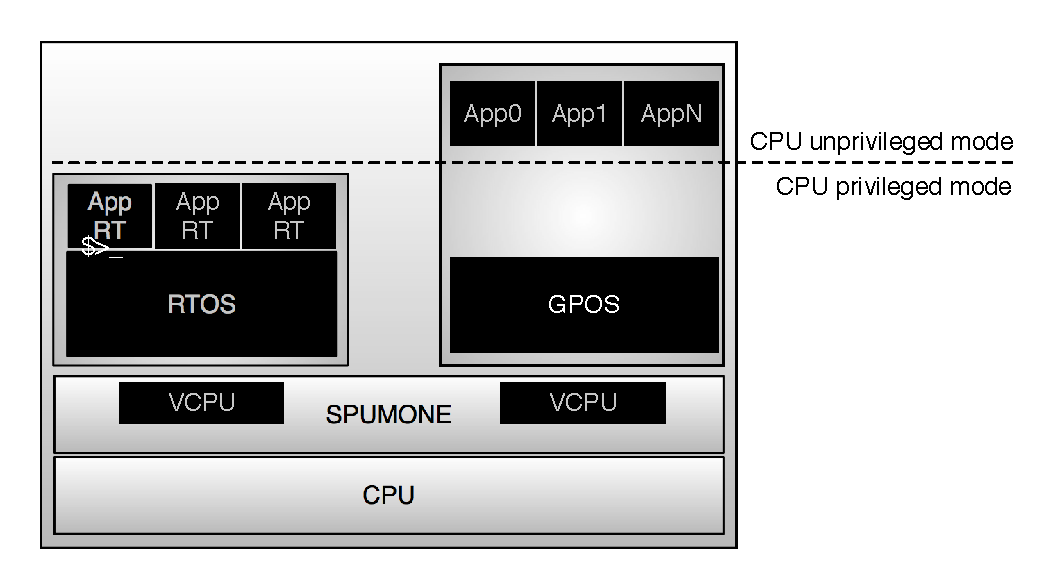
\includegraphics[width=.55\textwidth]{./chapter3/figures/spumone}
\caption{SPUMONE's single-core Architecture. Adapted from  \cite{spumone2008}.}
\label{fig:espumone}
\end{figure}

Mitake et al. \cite{hitoshi2011} proposed a distributed multicore architecture for SPUMONE as depicted in the Figure \ref{fig:espumone_multi}. Each CPU runs a SPUMONE instance and all guest kernels run at the privileged level. Each instance keeps a local memory area for data accessible only from local CPU. The authors claim that this design can reduce the intrusion risks at the virtualization layer, because a hypervisor instance is limited to one CPU. Additionally, this reduces the need of shared structures and synchronization among instances  increasing the scalability of the system. 

\begin{figure}[!hbtp]
\centering
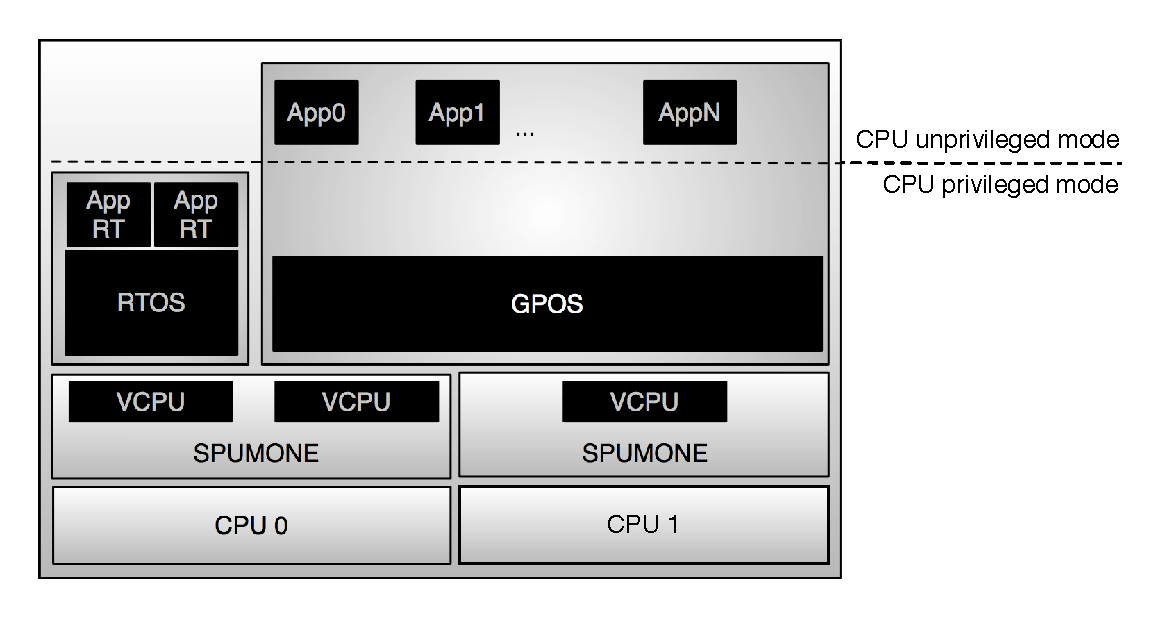
\includegraphics[width=.55\textwidth]{./chapter3/figures/spumone_multi}
\caption{SPUMONE's multicore Architecture. Adapted from \cite{hitoshi2011}.}
\label{fig:espumone_multi}
\end{figure}

In both SPUMONE versions (single and multicore), the authors chose better performance over reliability. Both RTOS and GPOS are complex software and can fail. For example, a faulty AppRT on the RTOS may compromise the whole system, because the hypervisor is at the same privilege level as the guest OS kernels. On the other hand, this approach decreases the number of hypercalls implemented in the guest OS, improving performance and maintainability.

In addition to the previously mentioned works, Mitake et al. \cite{mitake2012} proposed two new techniques to avoid the LHP problem (see Subsection \ref{subsection:holder}) in real-time virtualized systems using SPUMONE. These techniques rely on the VCPU migration among physical cores. The first technique called trap based migration consists in does not allow Linux to execute the kernel code on core 0 (see Figure \ref{fig:espumone_multi}). As the LHP is caused by the kernel's spinlocks, performing Linux kernel only on core 1 guarantee that the RTOS is performing concurrently with the Linux (see Figure \ref{fig:espumone_multi}). The second technique called on-demand migration consists in to migrate Linux from core 0 to core 1 when the RTOS executes on core 0 avoiding to execute the Linux and the RTOS on the same physical core. If the RTOS is addle, the Linux can perform on both cores. 


\section{XtratuM}
\label{section:XtratuM}

Crespo et al. \cite {xtratum2010} presented the XtratuM, a type 1 hypervisor specially designed for real-time embedded systems to meet temporal and spatial requirements of safety critical systems. In order to better fit real-time constraints, XtratuM was developed with the following a set of requisites: 

\begin{itemize}
\item data structures are static to allow for better control over the resources being used; 
\item XtratuM’s code is non-preemptive to make the code simpler and faster; 
\item all hypercalls are deterministic;
\item peripherals are managed by the VMs (directly mapped devices);  
\item interrupt occurrence isolation (when a VM is in execution only the interrupts related to it are enabled). 
\end{itemize}

\begin{figure}[!hbtp]
\centering
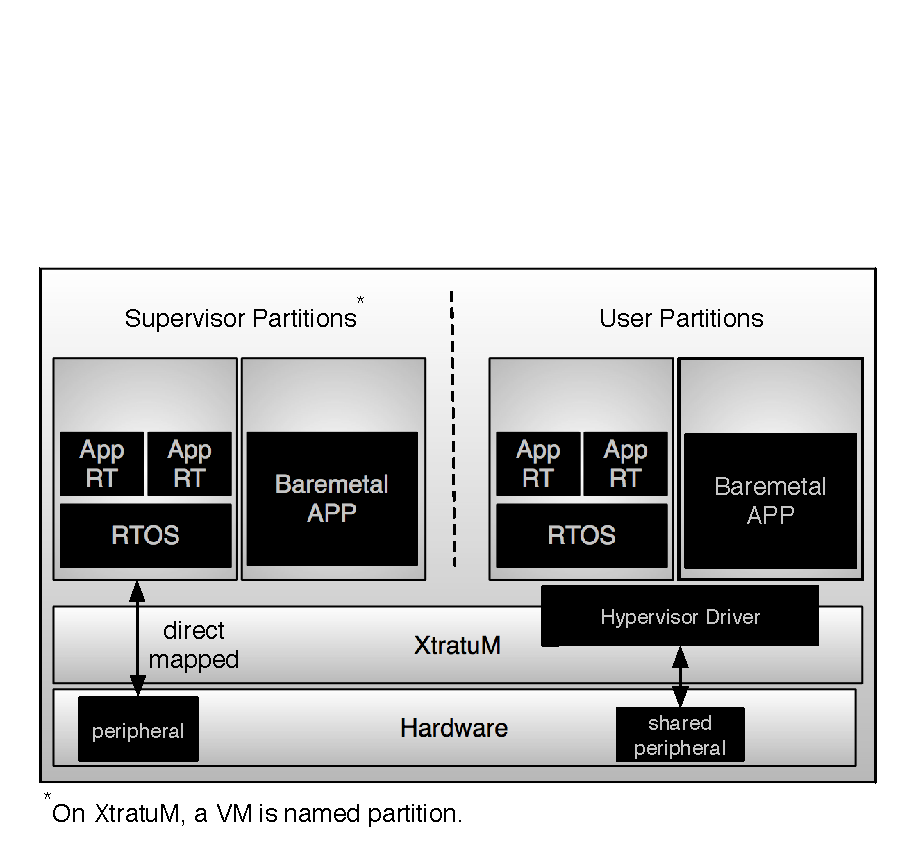
\includegraphics[width=.5\textwidth]{./chapter3/figures/XtratuM}
\caption{XtratuM's architecture. It is a type 1 hypervisor designed for safety critical systems. Adapted from \cite {xtratum2010}.}
\label{fig:XtratuM}
\end{figure}

Initially developed over x86, XtratuM now supports LEON2, LEON3, LEON4 (SPARC-V8 RISC \cite{sparkv8}) and ARM processor architectures. The hypervisor's overall architecture is shown in Figure \ref{fig:XtratuM}. In XtratuM, each VM is called a partition and each partition can support a RTOS or a bare metal application (GPOSs are not supported). There are two types of partitions: normal and system. Normal partitions have restricted functionality while system partitions can manage and monitor the state of the system and other partitions. Unlike SPUMONE, XtratuM  virtualizes not just the CPU and interrupts, but also some specific peripherals using para-virtualization. If there is no need to share a peripheral between two or more partitions, it can be directly mapped to the specific partition. When a peripheral needs to be shared between partitions, XtratuM implements a device driver to serialize the access and the guest OS must be modified in order to implement hypercalls to this device driver. 

In addition to previous work, Trujillo et al. \cite{trujillo2013} proposed the MultiPARTES: a project to support mixed critically integration for embedded systems based on virtualization techniques. It uses the XtratuM for virtualization purposes. MultiPARTES project resulted in a tool that allows for the application description using UML and additional annotations, like CPU time, memory, or bandwidth. The tool uses these descriptions to define a system partitioning and generate three outcome: source code, XtratuM configuration files, and system generation files. The authors claim that their approach accelerates the certification process for mixed-critical systems.


\section{L4 Microkernel Family based hypervisors}
\label{section:l4}

The microkernel concept reduces the OS kernel code to fundamental mechanisms and implements the remainder of the system services at the user level \cite{Liedtke1995}. The L4 microkernel was based on the L3 OS \cite{liedtke1993} developed by Liedtke to the x86 processor architecture. During his work at GDM and IBM, Liedtke modified the L3 to implement and test new ideas resulting in the L4. This initial development triggered an entire family of L4 based microkernels. Figure \ref{fig:timeline} summarizes the L4 microkernels family tree that resulted in embedded hypervisors. 

 

\begin{figure}[!hbtp]
\centering
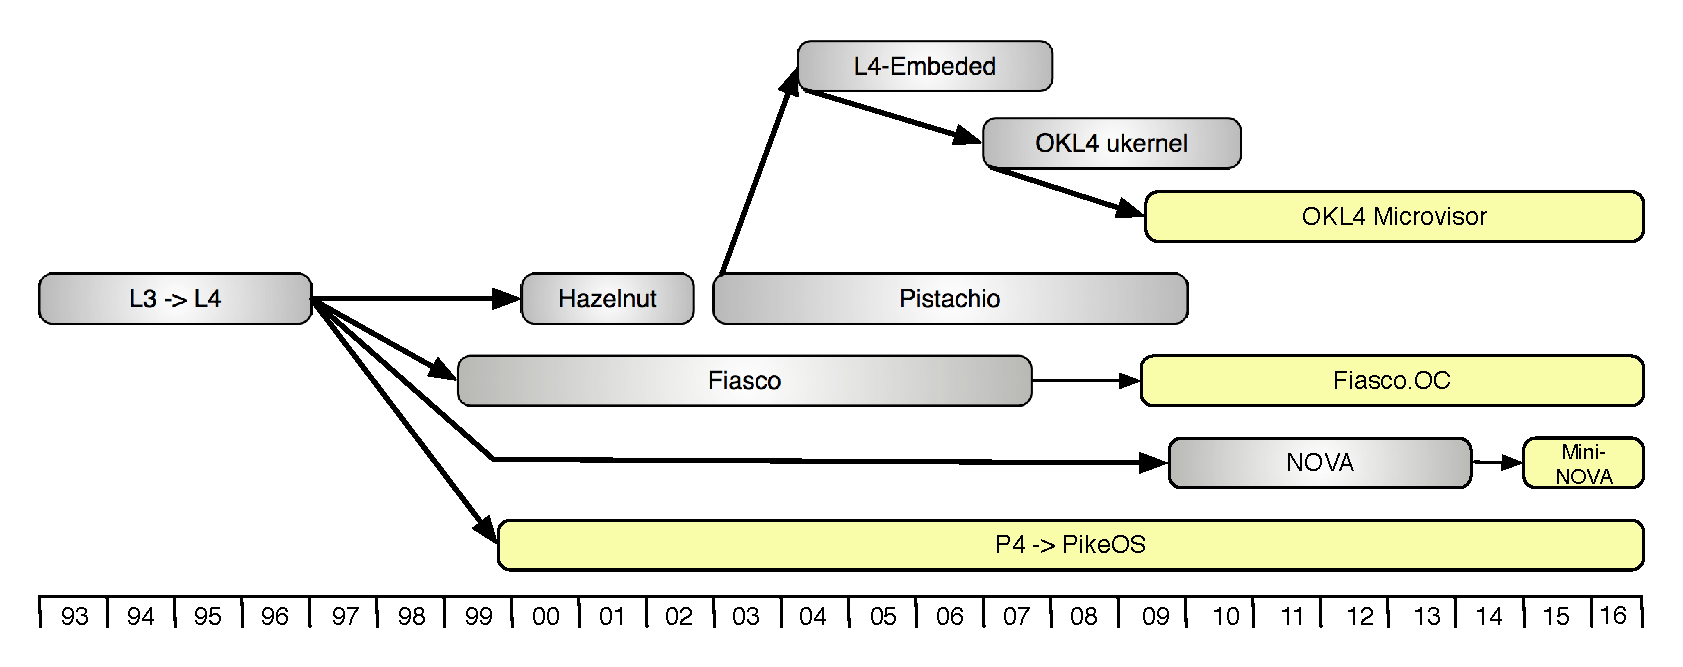
\includegraphics[width=.8\textwidth]{./chapter3/figures/l4-timeline}
\caption{Summarized L4 microkernel family tree that resulted in embedded hypervisors. Adapted from \cite{elphinstone2013}.}
\label{fig:timeline}
\end{figure}

GDM and IBM imposed a restrictive intellectual propriety for other researchers, forcing the University of Dresden to implement an x86 version of the L4 from scratch, called Fiasco. It was later renamed to Fiasco.OC. Liedtke moved to the University of Karlsruhe where he developed a version of the L4 supporting Pentium and ARM architectures, called Hazelnut. In 2001, it was implemented a new open-source kernel, called Pistachio, based on the previous version of L4. This kernel was written to x86 and PowerPC.  The NICTA Laboratory and the University of South Wales ported it to MIPS, Alpha, 64-bit PowerPC and ARM. NICTA created a fork of Pistachio, called L4-embedded, that was adopted by Qualcomm as an RTOS on wireless modems. The NICTA work resulted in a spin-off company called Open Kernel Labs for further support and development of the kernel. This company renamed L4-embedded OKL4 and developed the OKL4 Microvisor for virtualization purposes. PikeOS is another commercial clone of the original L4 that is certified for use in safety-critical avionics. NOVA is a open-source hypervisor based on L4 principles and designed for hardware-assisted virtualization on x86 platforms. Mini-NOVA is a port of the NOVA to the ARM Cortex-A9 using para-virtualization due to the absence of hardware support for virtualization on this processor. 


\subsection{OKL4 Microvisor}
\label{subsection:okl4}

The OKL4 Microvisor \cite{Heiser2010} was developed targeting mobile devices. Currently, it supports Linux, Android, Symbian and Windows Mobile OSs. The OKL4 powered the first commercial virtualized phone in 2009, named Motorola Evoke QA4. It executed two VMs on top of the OKL4 Microvisor: a Linux guest to handle the user interface and another guest for the BREW (Binary Runtime Environment for Wireless). 

Figure \ref{fig:okl4} shows OKL4's overall architecture. The microvisor is the only software layer that executes in the privileged mode while GPOSs, bare metal applications and even device drivers execute in the unprivileged mode. It has the ability to execute several GPOSs and bare metal applications concurrently. 

\begin{figure}[!hbtp]
\centering
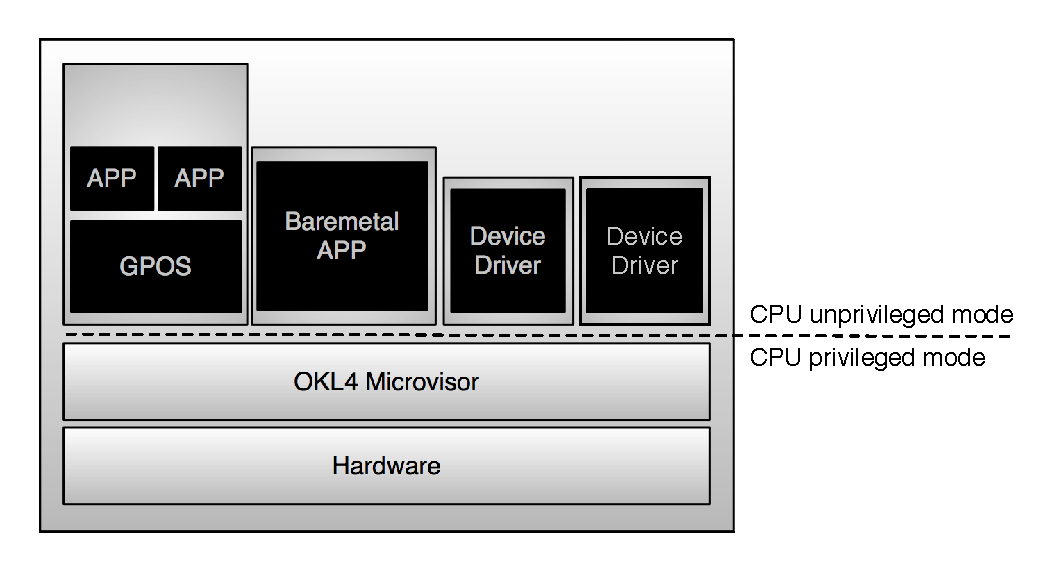
\includegraphics[width=.55\textwidth]{./chapter3/figures/okl4}
\caption{OKL4's architecture. It was developed targeting mobile devices supporting several mobile OSs, and it powered the first commercial virtualized phone in 2009.}
\label{fig:okl4}
\end{figure}

With OKL4 it is possible to execute both GPOS and a real-time environment on a single ARM processor, while providing high performance communication between them. This eliminates the need for a second ARM processor, which reduces the final cost and design complexity. 


\subsection{L4/Fiasco}
\label{subsection:fiasco}

The L4/Fiasco was developed as a clone of the original L4 kernel and adapted to provide virtualization on single-core x86 processors. Figure \ref{fig:fiasco} shows L4/Fiasco's architecture. L4Linux is a modified Linux kernel to support the L4/Fiasco's para-virtualization mechanism. It is mainly different from other hypervisors due to its  ability to map Linux kernel threads directly onto VCPUs. The L4Linux invokes hypercalls during kernel thread creation to allow to the L4/Fiasco to create VCPUs. However, this mechanism does not avoid the two-level scheduling problem because the Linux scheduler keeps mapping processes to Linux kernel threads. As is the case with other microkernels, device drivers are executed in user land. Additionally, L4/Fiasco supports RTOSs. 

%Confirmar se essa historia sobre o l4 Fiasco esta correta.

\begin{figure}[!hbtp]
\centering
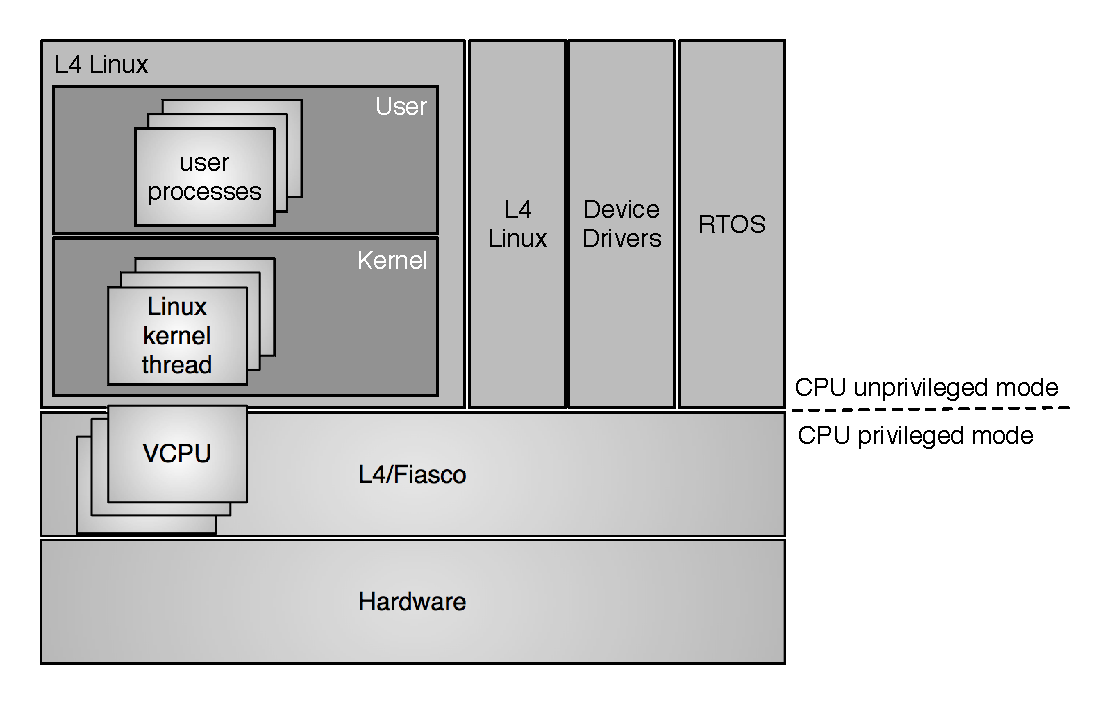
\includegraphics[width=.6\textwidth]{./chapter3/figures/fiasco}
\caption{Fiasco's architecture. The L4/Fiasco maps the L4Linux kernel threads directly to VCPUs.}
\label{fig:fiasco}
\end{figure}

Jungwoo et al. \cite{yang2011} proposed a compositional scheduling framework to deal with the two-level scheduling problem and extended  L4/Fiasco to support real-time constraints. L4Linux was modified to obtain the timing requirements from its internal processes and send them to the hypervisor through hypercalls. L4/Fiasco's scheduler implements a periodic task model and it uses the timing information from the guest OSs to meet the time constraints. This approach drastically reduces the number of deadline misses when compared to the original implementation. Additionally, it adds a small overhead that increases with the  number of threads. 


\subsection{PikeOS}
\label{subsection:pikeos}

PikeOS \cite{pikeos} is a proprietary microkernel developed by SYSGO AG\footnote{https://www.sysgo.com/} with support for virtualization. It was designed for safety-critical systems by implementing the concept of partitioning as defined by the ARINC 653 standard \cite{ARINC653}. Additionally, the standard determines the CPU time allocation across the partitions. The approach consists of a fixed cycle time in a specified order for a guaranteed duration. This allows for real-time guarantees, but it leads to a poor CPU utilization.  The microkernel has approximately 6,000 lines of code. It traps all interrupts and privileged instructions. Thus, it implements para-virtualization. Currently, it supports x86, PowerPCs and MIPS processors. 

\begin{figure}[!hbtp]
\centering
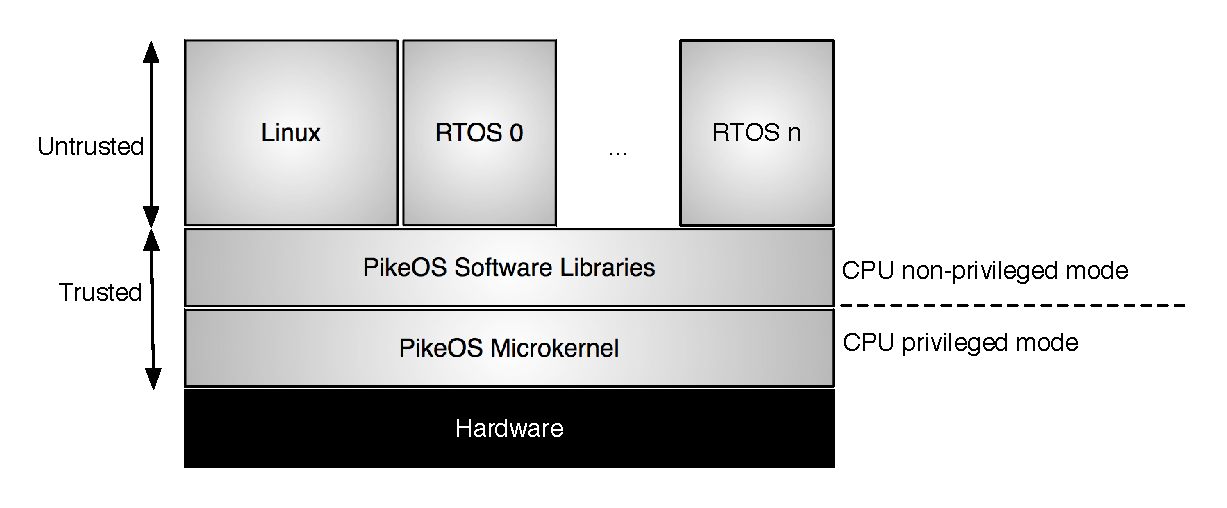
\includegraphics[width=.8\textwidth]{./chapter3/figures/pikeos}
\caption{PikeOS's architecture. It is a proprietary microkernel with support for virtualization designed to attend safety-critical systems.}
\label{fig:pikeos}
\end{figure}

Figure \ref{fig:pikeos} depicts the architecture of the PikeOS. The microkernel is the only software executed in CPU's kernel mode. The PikeOS software layers establish a set of partitions or VMs. Each partition can host a para-virtualized OS. The guest OSs are considered untrusted software and are kept isolated from each other. Finally, PikeOS supports inter-VM communication between guest OSs based on a mechanism defined by the ARINC standard. In this mechanism, the microkernel acts as a communication arbiter to manage message exchanges. 

\subsection{Mini-Nova}
\label{section:mini}

In 2010, Steinberg et al. \cite{Steinberg2010} proposed a hypervisor supporting the VT-x extensions on x86 architecture, called NOVA. Based on the NOVA hypervisor, Xia et al. \cite{Xia2015} suggested the use of the NOVA microkernel on an ARM-FPGA platform capable of managing reconfigurable hardware parts dynamically, but without support for virtualization. In the following work, Xia et al. \cite{tian2015} presented the Mini-NOVA, a type 1 embedded hypervisor for the ARM architecture using para-virtualization due to the absence of hardware support. 

The main difference in their approach is to  manage the coexistence of software and hardware computing resources. Thus, Mini-NOVA provides support for dynamic partial reconfiguration (DPR) to hardware tasks. According to the authors, the major challenge of this approach is to coordinate the hardware resources efficiently among the separate VMs. Security is another major concern, because the hardware tasks are shared among the guests. The solution adopts a centralized technique where a hardware task manager performs as a hypervisor service that manages the hardware. If a guest needs to execute a hardware task, it must require it using hypercalls. The evaluation demonstrated that the hardware can be efficiently managed with a short response latency and with a small overall latency. 


\section{M-Hypervisor}
\label{section:mhyper}

The M-Hypervisor \cite{rui2013} is a type 1 hypervisor supporting the Loongson 2f \cite{loogson2f} MIPS based processor. It is implemented by referencing the XtratuM's principles (see Section \ref{section:XtratuM}). Para-virtualization is adopted because Loongson 2f does not support the newer MIPS-VZ module. Hardware virtualization support is expected to be seen in the next generation of Loongson. Similar to XtratuM, the VMs are called partitions and support different OSs, like Linux and RTOSs. Real-time is supported through bare metal applications. The M-Hypervisor provides virtualization of the timer, interrupt, memory management, process switching and scheduling to ensure the real-time performance of high-level applications in the partitions and also temporal and spatial isolation. Based on the benchmarks, the authors claim that the M-Hypervisor can guarantee accurate real-time performance.


\section{Xvisor}
\label{section:xvisor}

Xvisor, shown in Figure \ref{fig:xvisor}, is an embedded hypervisor that supports both full-virtualization and para-virtualization\cite{patel2015}. It supports ARM virtualization extensions to provide full-virtualization and para-virtualization through optional VirtIO compatible device drivers. It can map interrupts directly to guests, allowing guest interrupts to be handled without the intervention of the hypervisor. Additionally, it provides memory isolation between hypervisor, guests and guest applications using the third privileged level from ARM's virtualization support. However, Xvisor has a poor support for MIPS processors since it only supports para-virtualization on the MIPS 24k processor model under the Qemu emulator.

\begin{figure}[!hbtp]
\centering
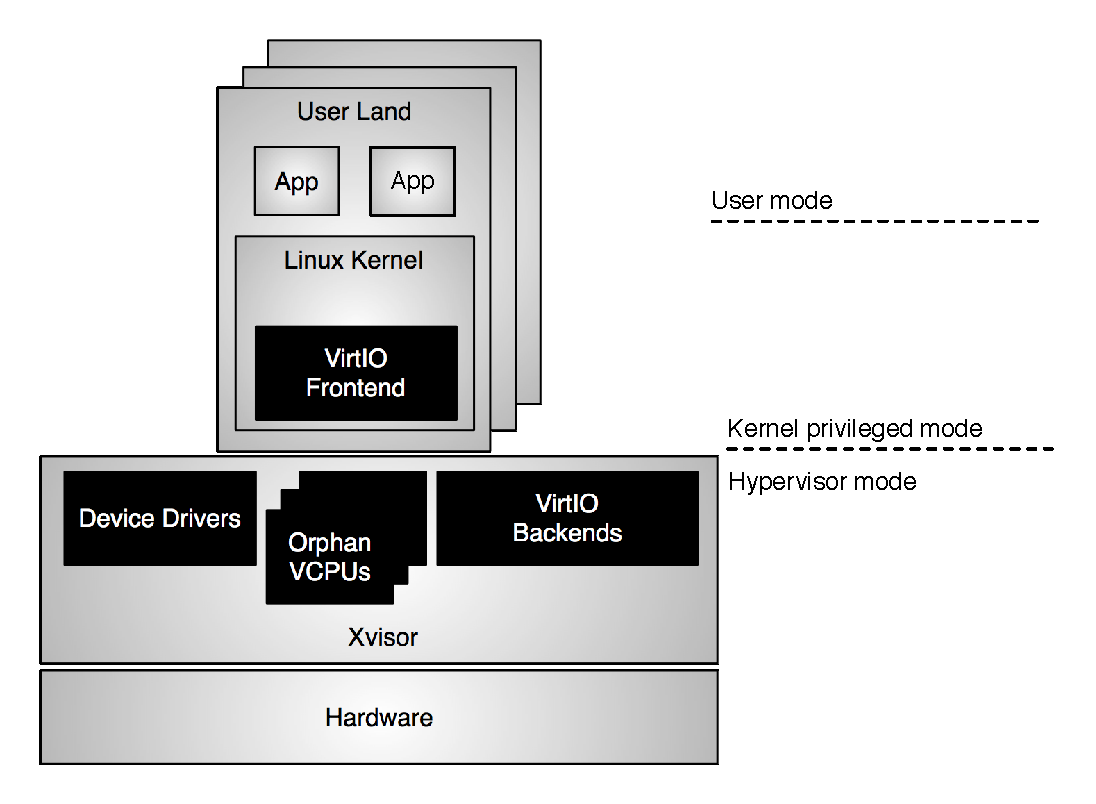
\includegraphics[width=.5\textwidth]{./chapter3/figures/xvisor}
\caption{Xvisor's architecture. The Xvisor hypervisor uses the third privileged level from ARM's architecture.}
\label{fig:xvisor}
\end{figure}

Xvisor implements the concept of Orphan VCPUs that executes background processing for device drivers and management purposes with the highest privilege. When compared to Xen or KVM, Xvisor has the advantage of having a single software layer where all virtualization related services are provided. For example, KVM depends on Qemu for device emulation and Xen depends on dom0 for I/O. Thus, the Xvisor's context switches are lightweight, resulting in instruction trap handling, host interrupts and guest I/O events. Also, the Xvisor's scheduler is per-CPU and does not do load balancing for multiprocessor systems. Instead, load balancing is performed by a distinct entity in Xvisor. 

\section{Embedded Hypervisors Comparison}
\label{section:comparative}

Table \ref{table:hypertable} is a comparison of the previously described embedded hypervisors and their key features. 

\begin{table}[!hbtp]
\caption{Embedded hypervisors' comparative table.}
\centering
\begin{tabular}{ p{2.5cm} p{3cm} p{3cm} p{3cm} p{3cm} l }
\hline\hline \\[-1.0ex]
\textbf{Hypervisor} & \textbf{Supported OSs} & \textbf{Architecture} & \textbf{Virtualization technique} & \textbf{Native Real-time support}\tablefootnote{Xen, KVM and L4/Fiasco can support real-time through modifications.} \\ [0.1ex]
\hline
Xen & Linux, Windows & ARM & PV, FV &  No \\ \hline
KVM & Linux, Windows & x86, ARM & PV, FV & No \\ \hline 
SPUMONE & Linux & SuperH-4A & PV & Yes \\ \hline
XtratuM & RTOSs & LEONx, ARM, & PV & Yes \\ \hline
OKL4 & RTOSs, Linux, Android & ARM, MIPS, x86 & PV & Yes\\ \hline
L4/Fiasco & Linux & x86(single-core) & PV & No\\ \hline
PikeOS & RTOSs & x86, PowerPC, MIPS & PV & Yes \\ \hline
Mini-NOVA & Linux, RTOSs & ARM & PV & Yes\\ \hline
M-Hypervisor & Linux, RTOSs & MIPS  & PV & Yes \\ \hline
Xvisor & Linux, RTOSs & ARM & PV/FV & Yes\\ \hline
\end{tabular}
\label{table:hypertable} 
\end{table}

The Xen hypervisor was developed for enterprise and desktop applications, as explained in Section \ref{section:xen}. However, recently it was ported to ARM processors. It does not support real-time natively. Instead, it requires modifications to improves the real-time responsiveness. Similar to Xen, KVM was recently ported to ARM processors and requires additional improvements in the Linux kernel to support real-time. All the other hypervisors presented were developed for embedded virtualization. However, with the exception of Xvisor, they were the first generation of embedded hypervisors. Thus, they share two important characteristics: lack of support for full-virtualization and lack of memory isolation between the guest's kernel and applications. Yet it is important to note that in SPUMONE the guest's kernel is executed in privileged mode along the hypervisor. Thus, it can keep the user applications isolated from each other, but the guest's kernel can access the hypervisor's memory space. Xvisor was designed to take advantage of the ARM virtualization support. Thus, it supports both full and para-virtualization and provides memory isolation between the hypervisor, guest kernel and guest applications. 

Tables \ref{table:footprintXenKvm} and \ref{table:footprintremain} compare the footprint of the hypervisors studied. Xen and KVM require the installation of additional elements to perform virtualization.  The installations column in Table \ref{table:footprintXenKvm} shows the different elements that must be installed with these hypervisors and their footprint. For example, Xen requires the Xen kernel, Dom0 and the Toolstack while KVM requires the Linux kernel and QEMU. Table \ref{table:footprintremain} compares the footprint of the remaining hypervisors.  
 
\begin{table}[!hbtp]
\centering
\caption{Footprint requirements for Xen and KVM.}
\label{table:footprintXenKvm}
\begin{tabular}{lccccc}
\hline \hline \\
                              & \multicolumn{3}{c}{\textbf{Installations}}                                    & \multicolumn{1}{l}{} \\ \\ \cline{2-4}
\multirow{2}{*}{\textbf{Xen}} & \textbf{Xen Kernel}        & \textbf{Dom0} & \textbf{Toolstack}   & \textbf{RAM}  & \textbf{footprint}\\
                              & 600KB \textgreater         & 3-4MB                    & 20MB \textless      & 180MB\textgreater   & 204MB\textless\\ \\\hline
\multirow{2}{*}{\textbf{KVM}} & \textbf{Host Linux zImage} & \textbf{QEMU}             & \multicolumn{1}{l}{} & \multicolumn{1}{l}{} & \textbf{footprint}\\
                              & 3-4MB                     & 20MB \textless           &                      & 20MB \textgreater & 44MB\textless   \\ \hline
\end{tabular}
\end{table}

Xen has a total footprint of roughly 204MB. KVM has a smaller footprint, but it requires a host Linux to execute. When compared to the configuration of modern computer servers, these requirements are modest. However, though they are used in embedded systems, their footprint may be unacceptable for many devices. 

\begin{table}[!hbtp]
\centering
\caption{Footprint requirements of the hypervisors when available.}
\label{table:footprintremain}
\begin{tabular}{llll}
\hline \hline \\
                     & \multicolumn{1}{c}{\textbf{kernel size}} & \multicolumn{1}{c}{\textbf{RAM Memory}} & \multicolumn{1}{c}{\textbf{footprint}}\\ \\ \hline
\textbf{SPUMONE}              & 30KB                                         &  - & >30KB\tablefootnote{The total memory needed by SPUMONE during its execution is unknown.}                                       \\
\textbf{Xtratum} & 8KB                                      & 16KB         & 24KB                            \\
\textbf{OKL4}                 & 48KB                                     & 78KB         & 126KB                           \\
%\textbf{L4/Fiasco}            &                                          &                                         \\
%\textbf{PikeOs}               &                                          &                                         \\
\textbf{Xvisor}               & 1-2MB                                    & 4-16MB       & 5-18MB                           \\
\textbf{Mini-NOVA}              & 40KB                                    & 20MB        & 20.04MB                         \\ \hline
\end{tabular}
\end{table}

Hypervisors developed for embedded systems typically present a smaller footprint than hypervisors for server virtualization. Unfortunately, some authors do not mention the memory requirement of their hypervisors. This is the case for L4/Fiasco, PikeOs and M-Hypervisor. The remaining of the hypervisors are shown in Table \ref{table:footprintremain}. Note that the footprint and RAM requirements can be quite different. For example, Xvisor has a footprint between 5 and 18MB. OKL4 has a footprint of only 126KB. SPUMONE's kernel requires 30KB each core in its multicore version. For example, in a dual-core processor SPUMONE will require 60KB. However, the amount of memory needed during its execution is unknown. Xtratum has the smallest footprint, requiring only 24KB during its execution.


\section{RT-Linux}
\label{section:rtlinux}

RT-Linux \cite{cottet2002} provides the capability of executing bare-metal tasks along a Linux OS. It is a kernel patch that adds a software layer with a real-time scheduler. From the point of view of the RT-Linux layer, the Linux kernel is a process that shares the processor with real-time tasks. Figure \ref{fig:rtlinux} shows RT-Linux's architecture. The I/O and interrupts subsystems of the Linux kernel are modified to communicate with the RT-Linux layer. This is similar to a para-virtualized hypervisor. The bare-metal tasks have priority over the Linux kernel and can access peripherals directly. Additionally, the Linux kernel will always be pre-empted to give priority to the real-time tasks. 

\begin{figure}[!hbtp]
\centering
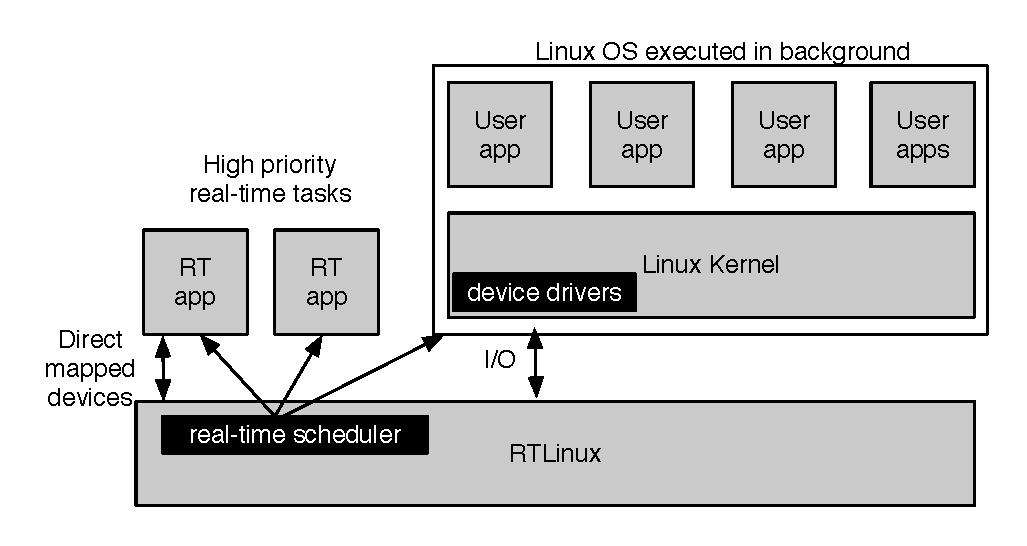
\includegraphics[width=.6\textwidth]{./chapter3/figures/rtlinux}
\caption{RT-Linux is a kernel patch that adds a software layer with a real-time scheduler and it makes the Linux kernel to share the processor with real-time tasks.}
\label{fig:rtlinux}
\end{figure}

RT-Linux's architecture is similar to a lightweight hypervisor, but without the capability of supporting multiple guest OSs. In fact, its objective is to improve the responsiveness of real-time tasks while maintaining the Linux software stack. The real-time tasks must be written using the RT-Linux API. Finally, shared memory can be used for communication between real-time tasks the Linux threads. 

\section{Final Considerations}
\label{section3:considerations}

This chapter presented the main hypervisors available for embedded virtualization. This study exposed the complexity of  embedded virtualization and the wide range of possible solutions. It was identified that real-time is an issue addressed frequently, since all mentioned hypervisors have some real-time support. In respect to Xen and KVM, the primary focus of the studied works is the issue of real-time improvements. These hypervisors have a deep dependency on the Linux OS, which makes it difficult to reduce their memory requirements. Thus, a recurrent challenge for hypervisors specially designed for embedded systems is to achieve a small footprint. To accomplish this goal, they avoid dedicating domains for I/O (in contrast  to Xen) and they implement the type 1 hypervisor model (unlike KVM).  Also, the presented hypervisors regularly do not meet common embedded system requirements. For example, XtratuM does not support GPOSs while SPUMONE cannot provide spatial isolation between guests. L4 based hypervisors support GPOSs and provide spatial separation but do not support full-virtualization. Para-virtualization is extensively adopted on embedded hypervisors. As seen in Table \ref{table:hypertable}, KVM and Xvisor are the only embedded hypervisors that support full-virtualization, but their support is limited to the ARM virtualization extensions. Chapter \ref{chapter:background} showed that hardware-assisted virtualization is a trend in embedded processors. Thus, it is inevitable for the further development on hypervisors to adopt full-virtualization even when combined with para-virtualization. This study makes it clear that an novel embedded virtualization model is required to take advantage of newer processors and to better fit embedded system needs.


%trabalho que precisam ser analizados

%XEN

%2012 - Credit-based Low Latency Packet Scheduling Algorithm for Real-time Applications 



%KVM/ARM: The Design and Implementation of the Linux ARM Hypervisor

%KVM

%NV-CFS: NVRAM-Assisted Scheduling Optimization for Virtualized Mobile Systems - http://ieeexplore.ieee.org/xpl/articleDetails.jsp?arnumber=7336257&queryText=KVM%20EMBEDDED&sortType=desc_p_Publication_Year&searchField=Search_All

%Responsive and Enforced Interrupt Handling for Real-Time System Virtualization - http://ieeexplore.ieee.org/xpl/articleDetails.jsp?arnumber=7299849&queryText=KVM%20EMBEDDED&sortType=desc_p_Publication_Year&searchField=Search_All

%Platform Device Assignment to KVM-on-ARM Virtual Machines via VFIO - http://ieeexplore.ieee.org/xpl/articleDetails.jsp?arnumber=6962282&queryText=KVM%20EMBEDDED&sortType=desc_p_Publication_Year&searchField=Search_All

%Processor virtualization on embedded linux systems - http://ieeexplore.ieee.org/xpl/articleDetails.jsp?arnumber=6924360&queryText=KVM%20EMBEDDED&sortType=desc_p_Publication_Year&searchField=Search_All

%SPUMONE

%A Light-Weighted Virtualization Layer for Multicore Processor-Based Rich Functional Embedded Systems - http://ieeexplore.ieee.org/xpl/articleDetails.jsp?arnumber=6195872&queryText=SPUMONE&sortType=desc_p_Publication_Year&searchField=Search_All

%Using Virtual CPU Migration to Solve the Lock Holder Preemption Problem in a Multicore Processor-Based Virtualization Layer for Embedded Systems - http://ieeexplore.ieee.org/xpl/articleDetails.jsp?arnumber=6300159&queryText=SPUMONE&sortType=desc_p_Publication_Year&searchField=Search_All


% l4 family three - http://www.disy.cse.unsw.edu.au/projects/kernel/

%l4 fiasco - http://moss.csc.ncsu.edu/~mueller/rt/rt11/readings/projects/g3/report3.pdf

% Implementation of Compositional Scheduling Framework on Virtualization 


%AUTOSTAR

%http://ieeexplore.ieee.org/xpl/login.jsp?tp=&arnumber=6871203&url=http%3A%2F%2Fieeexplore.ieee.org%2Fstamp%2Fstamp.jsp%3Ftp%3D%26arnumber%3D6871203

%Takumi Shimada1
%http://ieeexplore.ieee.org/stamp/stamp.jsp?tp=&arnumber=7396874


\chapter{\label{chapter:vtmodel}A Virtualization model for embedded systems}

This chapter presents the virtualization model proposed by this dissertation. As discussed in Subsection \ref{section3:considerations}, the techniques currently applied for virtualization on embedded environments do not meet all requirements. Additionally, the evolution of the embedded processors is growing towards the usage of hardware support for virtualization. However, this is ongoing, and the next generations of embedded processors will support new hardware features for virtualization. Thus, the existing virtualization techniques for ES require continuous improvement and new approaches must be proposed. Based on the state-of-the-art for embedded virtualization, a set of important features were chosen as a guideline for the development of embedded virtualization models. Section \ref{section4:desirable} discusses these features. Section \ref{section:propose} presents the proposed virtualization model. The Embedded Systems Group (GSE) started to research embedded virtualization in 2010. Since then, another virtualization model was proposed by Aguiar \cite{aguiar2013}. Thus, Section \ref{section:vhh} compares the virtualization model presented in this dissertation to the model proposed by Aguiar \cite{aguiar2013}. Finally, Section \ref{section:final4} is the final considerations of this chapter. 

\section {Desirable Features for an Embedded Virtualization Model}
\label{section4:desirable}

This section states the important features for an embedded virtualization model. As explained before, real-time support on virtualized ESs has become an major concern, since all works presented in Chapter \ref{chapter:stateofart} have some support for real-time. However, these works still have different drawbacks. Widely adopted hypervisors like Xen and KVM (see Subsections \ref{section:xen} and \ref{section:kvm}) were designed for enterprise usage and do not scale well on some ESs because of their memory footprint. Solutions designed to target ESs, like SPUMONE, XtratuM and L4/Fiasco (see Sections \ref{section:spumone}, \ref{section:XtratuM} and \ref{subsection:fiasco}) have different constraints. For example,  SPUMONE does not provide spatial isolation, XtratuM was designed for critical systems, therefore it does not support GPOSs, and L4/Fiasco was designed for only single-core processors and it does not have proper real-time support. Moreover, the most of the hypervisors do not make use of the current hardware-assisted support present in the modern embedded processors. The only exception is the Xvisor (Section \ref{section:xvisor}), but its support is restrict to ARM processors. The research shows an increasing interest in emergent topics like hardware-assisted virtualization and security. Thus, it is essential to address these topics on a virtualization model. 

Based on the related works, there is not a consolidated approach for embedded virtualization. Additionally, due to the wide diversity of ES architectures and applications, there is not a single approach that can overcome all challenges at once. Nevertheless, more accurate techniques can be applied to build a hypervisor able to better address the virtualization needs on the most of ESs. Thus, this dissertation suggests a virtualization model that supports the following major features:

\begin{itemize}
\item \textbf{Hardware-assisted virtualization}: Considering that virtualization will be widely adopted for ESs shortly, the manufacturers will provide hardware-assisted virtualization for their embedded CPUs. The decreased fabrication cost of the embedded processors allowed for the adoption of hardware features for virtualization support. In fact, ARM and MIPS have already specified their  virtualization extensions as seen in \cite{armvt} and \cite{mipsvz}. Additionally, several manufacturers have released their virtualization platforms. Once the hardware supports a flexible set of features, hypervisor designers must decide what policy usage to adopt. As explained in Subsection \ref{subsection:hardware-assisted}, hardware-assisted virtualization allows more efficient and simpler hypervisors. The main advantages of the hardware-assisted virtualization are to speed-up hypervisor performance, save engineering costs and improve time to market.

\item \textbf{Multicore support}: Multicore processors are already widespread in ES platforms. When available, the hypervisor should ensure the proper support to obtain maximum performance. Additionally, migration of VCPUs between physical cores should be considered to allow load balancing. 

\item \textbf{Real-Time support}: Real-time is an intrinsic characteristic of embedded systems. The hypervisor should be predictable and ensure temporal isolation between GPOS and real-time applications. For multimedia purposes, soft real-time support is enough. Nevertheless, some ESs require accurate time constraints to run with GPOSs. For example, a smartphone system that must support a rich user graphical interface still needs to deal with the GSM stack \cite{appleton1998} time constraints. In this case, real-time support is desirable because it avoids the need for a second processor dedicated to the GSM stack.

\item \textbf{Coexistence of multiple GPOSs and Real-time instances}: A GPOS is highly desirable for certain ESs, such as smartphones and set-up boxes, due to its wide diversity of software. However, usually GPOSs have poor real-time responsiveness. In fact,the hypervisor must guarantee real-time instances that are executed with GPOSs. Additionally,  some virtualized platforms can require more than one GPOS at the same time. For example, in a virtualized network router that, for reliability reasons, the data plan must be isolated from the control plan. 

\item \textbf{Direct mapped and shared devices}: The current generation of embedded platforms designed for virtualization do not support I/O virtualization. Thus, when it is necessary to share a physical device, e.g. an Ethernet device, the hypervisor may use the para-virtualization technique. In this case, a device driver at hypervisor level serializes the access to the Ethernet device, and the guest OS implements a para-virtual device driver. However, aiming better performance, when device sharing is not desired, the hypervisor must map the device directly to the desired guest OS. Efficient implementation of directly mapped devices depends on the support of the processor's hardware (see Subsection \ref{subsection:interrupt}).

\item \textbf{Security}: The hypervisor must provide robust spatial isolation between VMs, i.e., a misbehavior in the guest OS should not affect the behavior of the other guest OSs or even the hypervisor. The goal of separation used for security purposes is to create and preserve a trusted operating environment for an embedded system. Separation is intended to prevent exploitable defects in one virtualized environment from propagating to adjacent virtual environments, or to the physical platform as a whole \cite{security-prpl}.

\item \textbf{Inter-VM communication}: A virtualized system is composed by a set of VMs. Possibly, these VMs will require some level of interaction between them. Also, some applications can require secure communication channels for sensitive information. Thus, an efficient and secure inter-VM communication mechanism must be available in the hypervisor.

\item \textbf{Lightweight virtualization layer}: Due to the resource constraints on ESs, the hypervisor layer must have a small memory footprint and induce the least amount of overhead possible. This requirement is intrinsically related to hardware-assisted virtualization. As explained in Section \ref{subsection:hardware-assisted}, greater hardware support simplifies hypervisor implementation and can improve performance.   
\end{itemize}

The design of an embedded hypervisor should consider this features. However, some are difficult to measure. For example, if the hypervisor is lightweight, it cannot be measured directly, but it can only be compared regarding the lines of code and memory footprint of similar hypervisors. Security is another feature that is hard to evaluate. The simplest way to evaluate security is to consider if the hypervisor ensures spatial isolation or separation between VMs. However,  critical systems may require formal proof. Other system characteristics are directly measured based on responsiveness, memory and time overhead. Section \ref{section:propose} presents the proposed virtualization model that is flexible enough to accommodate these features. 



\section{Model Overview}
\label{section:propose}

An innovative virtualization model was proposed based on the desired features described in the Section \ref{section4:desirable}. As a result, an implementation of this model is presented in the Chapter \ref{chapter:implementation}. Thus, this section describes the proposed virtualization model. However, there are two considerations about this model:

\begin{enumerate}
  \item The model does not try to impose or improve the real-time capabilities of non real-time entities, like a GPOS. Instead, it provides mechanisms for GPOSs and real-time entities coexist and;
  
  \item The model was not designed to be a pure full-virtualization model. Instead, it was designed to support full-virtualization of the CPU and use the para-virtualization concept for other services, such as communication and shared devices.
\end{enumerate}

Many hypervisor solutions for ESs try to improve the real-time responsiveness of GPOSs in virtualized environments. For example, different authors propose to apply techniques to improve the Linux real-time responsiveness when virtualized in KVM or Xen (see sections \ref{subsection:kvmproposals} and \ref{subsubsection:xenproposals}). However, the proposed model avoids the utilization of GPOSs as real-time instances. Instead, it allows real-time services to be directly scheduled by the hypervisor, see Subsection \ref{subsection4:realtime}. Additionally, the model provides full-virtualization based on the hardware-assistance of the CPU. Other peripherals may require para-virtualization techniques, see Subsection \ref{subsection4:services}.  

Figure \ref{fig:virtmodel} depicts the proposed model. At the hardware level, it uses a bus-based homogeneous MPSoC along with shared memory. The first software layer is the the hypervisor, which is responsible for the creation and management of each VM. It also provides a logic arrangement for associating the VM with its VCPUs. Moreover, the hypervisor controls the memory space of each VM for memory isolation. Thus, this model describes a hypervisor type 1, as explained in Subsection \ref{subsection:hypertypes}. Type 1 hypervisors usually requires lower footprint then type 2 ones, since they does not require an underline OS. 

\begin{figure}[!hbtp]
\centering
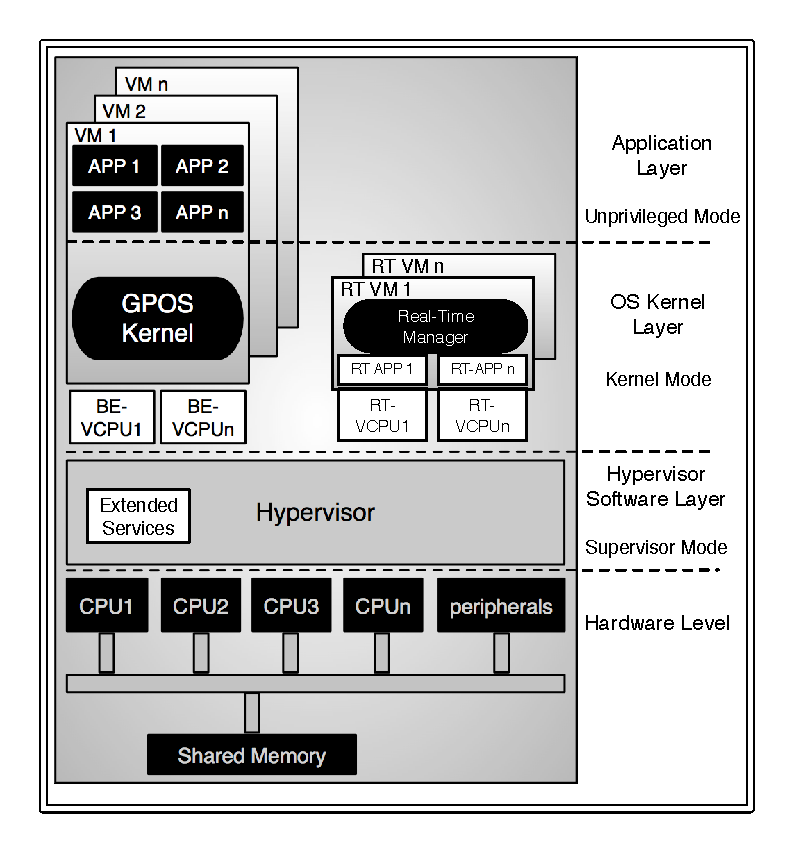
\includegraphics[width=.45\textwidth]{./chapter4/figures/hypervisormodel}
\caption{Overall view of the proposed virtualization model.}
\label{fig:virtmodel}
\end{figure}

The GPOSs are mapped onto best-effort VCPUs while real-time instances are mapped onto real-time VCPUs, as further explained in Subsection \ref{subsection:flex}. The model takes advantage of the processor's additional privilege levels (see Subsection \ref{subsubsection2:privelege}) to provide spatial isolation between hypervisor and guests. Additionally,  unlike virtualization models that do not utilize the additional privilege levels scheme, the proposed model can provide spatial isolation between the guest kernel and guest applications. Therefore, the hypervisor is protected from the actions of malicious or misbehaving guest OSs and the guest OSs are protected from their applications. 

The model provides additional features, called extended services, that expand the virtualization platform functionalities. See Subsection \ref{subsection4:services} for more details. Additionally, for better temporal isolation, the model proposes the adoption of the RT-VM, which maps real-time services onto RT-VCPUs, as explained in Subsection \ref{subsection4:realtime}. Finally, direct communication among VMs is possible using shared memory areas or message passing mechanisms can be implemented using the hypervisor as a communication arbiter, which is explained in detail in Subsection \ref{subsection4:comm}.


\subsection{The Flexible Scheduling Mapping}
\label{subsection:flex}

Figure \ref{fig:mappingmodel} shows the possible flexible mapping and the partitioning model for virtualized architectures based in the proposed model. To perform temporal isolation between VMs, the hypervisor specifies two different kinds of VCPUs:  best-effort VCPUs (BE-VCPUs) and real-time VCPUs (RT-VCPUs). RT-VCPUs have priority over BE-VCPUs and follow the policy of a real-time scheduling algorithm. BE-VCPUs are scheduled by a best-effort scheduler algorithm that is invoked when there are not RT-VCPUs ready to execute. Additionally, the BE-VCPUs can migrate among physical cores, i.e., when a CPU becomes idle the scheduler will choose the next BE-VCPU ready to run in a global queue. The migration of RT-VCPUs depends on the real-time scheduler algorithm adopted. Due to time constraints, a real-time scheduler algorithm for multicore processors must be carefully designed, as proposed by \cite{saranya2015} and \cite{vigeant2015}. This model is flexible enough to accommodate different combinations of real-time and best-effort scheduler algorithms, which is an implementation decision. 

\begin{figure}[!hbtp]
\centering
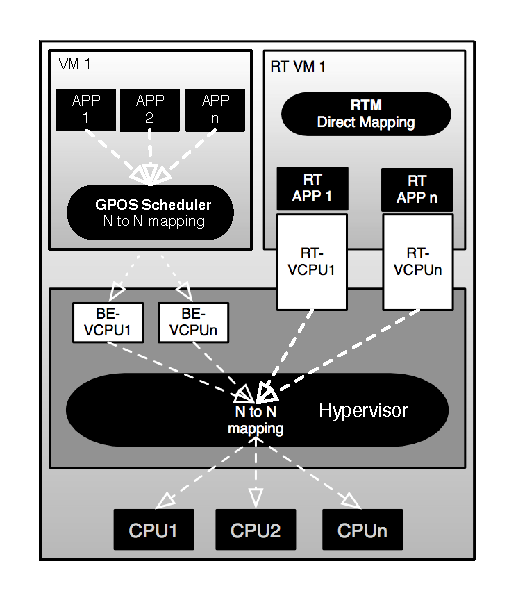
\includegraphics[width=0.45\textwidth]{./chapter4/figures/flexiblemapping}
\caption{Flexible mapping for multiprocessor embedded systems with real-time support.}
\label{fig:mappingmodel}
\end{figure}

A multiprocessing GPOS may have several BE-VCPUs available, and its scheduler is responsible for mapping the task among BE-VCPUs according to its policies. At the hypervisor level, the best-effort scheduler algorithm will map a BE-VCPU to the next idle CPU. This arrangement enables an N-to-N mapping of task over BE-VCPUs and BE-VCPUs over CPUs. 


\subsection{Extended Services}
\label{subsection4:services}

The model suggests the implementation of the para-virtualization concept to provide extended services to the guest OSs. Extend services are useful to expand the virtualization platform functionalities, i.e., to implement functions that does not exist in a pure fully-virtualized system. Hypercalls are widely used in para-virtualization based approaches, where the guest OS needs to be modified to invoke hypercalls instead of using privileged instructions. However, this work uses  full-virtualization with a hardware-assisted technique, where the guest OS does not need to be modified for virtualization purposes.  Yet it must use hypercalls to take advantage of the  extended services, e.g., real-time services and communication among VMs. 

The model suggests a minimal set of extended services. However, an implementation can add services for different purposes as necessary. Table \ref{table:hypercalls} resumes the extended services available through hypercalls. Altogether, six different hypercalls are supported and may be implemented by a guest OS when needed. The services are divided into three different groups:

\begin{itemize}
    \item VM identification composed by a hypercall that returns a unique VM identification number issued by the hypervisor.
    \item RT-VCPU management is composed by a group of three hypercalls responsible to manage the RT-VCPUs. Using this hypercalls the guest OS can create, launch or delete  real-time services.  
    \item Communication services are composed of two hypercalls designed for communication purposes.
\end{itemize}


\begin{table}[!hbtp]
\caption{Hypercalls as extended services.}
\centering
\begin{tabular}{l l l}
\hline\hline \\
\textbf{Extended Service} & \textbf{Hypercall} & \textbf{Description} \\ 
\hline \\
VM identification & HCALL\_INFO\_GET\_ID  & Return the VM ID number  \\
\hline
\multirow{3}{*}{RT-VCPU  Management} & 
    HCALL\_RT\_CREATE\_APP & RT application Instantiation  \\
    & HCALL\_RT\_LAUNCH\_APP & RT application launch  \\
    & HCALL\_RT\_DELETE\_APP & RT application delete \\
    \hline
\multirow{2}{*}{Communication Services} & 
     HCALL\_IPC\_SEND\_MSG  & Send messages \\ 
    & HCALL\_IPC\_RECV\_MSG & Receive messages \\ \hline
\end{tabular}
\label{table:hypercalls} 
\end{table}

The utilization of the hypercalls for management  of the RT-VCPUs is better explained in Subsection \ref{subsection4:realtime}. The extended services proposed in Table \ref{table:hypercalls} are supported by the hypervisor implementation presented in Chapter \ref{chapter:implementation}.

\subsection{Real-time Aspects}
\label{subsection4:realtime}

To deal with real-time constraints, a special VM called RT-VM was designed to provide a robust temporal isolation between real-time services and GPOSs. The RT-VM does not support RTOSs. Instead, it implements what is  called a Real-Time Manager (RTM), which supports communication facilities and basic user libraries. The RTM can map its tasks directly to RT-VCPUs in the hypervisor scheduler, i.e., it does not implement a scheduler on its level avoiding the hierarchical scheduling problem and improving performance. The real-time services must be registered during the RT-VM initialization calling the HCALL\_RT\_CREATE\_APP hypercall. After the registration, the real-time services are available in the system and they can be started/stopped by the guests using the hypercalls HCALL\_RT\_LAU\-NCH\_APP and HCALL\_RT\_DELETE\_APP. 

RTM may or not provide spatial isolation between tasks. Providing spatial isolation means the implementation of virtual memory support on the RTM, which may impact in the real-time responsiveness. Nevertheless, if spatial isolation between different services is desired, more than one RT-VM can be instantiated. When a developer is interested in taking advantage of real-time in this model, he must implement its real-time service using the RTM API.

The RT-VCPUs are scheduled by a real-time algorithm, e.g., EDF, which has priority over the best-effort scheduling algorithm. To keep the RT-VCPUs in a global queue (allowing migration) or in a local queue per CPU is a implementation decision. As described in Subsection \ref{subsection:flex}, an implementation for multi-core processor using a global queue and allowing CPU migration must be carefully designed to guarantee temporal isolation. Additionally, critical systems require schedulability analysis to guarantee system resource availability during RT-VCPU admission. Finally, during the execution of a RT-VCPU, interrupts sent to BE-VCPUs may or not be postponed in order  to increase temporal isolation, see Section \ref{section5:interrupt} about interrupt delivery policies.

\subsubsection{Schedulability Analysis for Real-time Services}

As explained, the real-time services are available in the RT-VM, and they can be started/stopped by the guest OSs. An important concern about this scheme is how to deal with concurrent real-time services that can be started asynchronously. For example, a set of real-time services available in a RT-VM may not be schedulable altogether. Thus, some of the real-time services may not be accepted for execution when a guest OS requires it due to unavailable CPU time. This is especially critical for systems where the non-execution of a service may cause safety concerns. 

The model does not specify mechanisms for schedulability analysis or any other approach to avoid the schedulability problem. In fact, to determine the schedulability of a task set, the real-time scheduling algorithm and the real-time scheduling parameters must be known. However, the model allows for different real-time algorithms making the schedulability analysis dependant of implementation. Finally, the simpler approach for a hypervisor based on this model to avoid schedulability problems is to guarantee the schedulability of the set of real-time services available in the system. For this, two approaches can be take: 

\begin{itemize}
    \item The development team performs a schedulability analysis;
    \item The hypervisor implements its own schedulability test, that is performed during its initialization. 
\end{itemize}

Both approaches can be used together. If the development team fails in their schedulability analysis, the hypervisor can detect the problem during the system's initialization, since the RT-VM must register its services at boot time using the hypercall HCALL\_R\-T\_CREATE\_APP. It is important to highlight that both approaches work only for real-time services implemented at design time. However, the model does not permit to install new real-time services in runtime. The hypervisor implementation presented in Chapter \ref{chapter:implementation} implements the schedulability test to the EDF scheduler algorithm. 

\subsection{Communication Model}
\label{subsection4:comm}

Inter-VM communication capabilities must be implemented as part of the extended services, i.e., using hypercalls. However, the model does not impose any specific communication mechanism. Instead, this decision is made by the developer. For example, for better performance, the designers may choose to implement direct communication between VMs using memory sharing. Or, if the major concern is security, the designers may choose to implement a message exchange mechanism using the hypervisor as a communication arbiter. The model's implementation presented in Section \ref{chapter:implementation} provides communication between VMs using the hypervisor as a manager.  

Inter-device communication, i.e., communication of the virtualized platform with external devices is desirable in modern ESs. The proposed model is flexible enough to support typical socket style \cite{tanenbaum2011} communication among VMs. Thus, the hypervisor may implement a network layer in order to route Internet Protocol (IP)  datagrams \cite{tanenbaum2011} between VMs. Still, when communication with the external world is desired, the hypervisor may virtualize a network adapter providing network capabilities to the platform. Nevertheless, in the embedded system context, the socket communication scheme can be expensive in terms of system overhead, therefore message passing may be preferable.

\section{Comparison with the Virtual Hellfire Hypervisor (VHH)}
\label{section:vhh}

In 2010, the GSE group started to research virtualization for embedded systems. Aguiar \cite{aguiar2013}, proposed an embedded virtualization model and a hypervisor implementation in 2013. The resulting hypervisor was called Virtual Hellfire Hypervisor (VHH). This section discusses the main differences between the virtualization model proposed by Aguiar and the model presented in this dissertation. 

Figure \ref{fig:vhhmodel} presents the VHH's virtualization model. Similar to the model proposed in this dissertation, the VHH model assumes a bus-based homogeneous MPSoC along with shared memory. On top of the CPUs, it executes the hypervisor, which is responsible for the creation and management of each Application Domain Unit (ADU). The ADU is a logical arrangement responsible for associating the guest OS with its VCPUs. Moreover, each ADU has its own memory space controlled by the hypervisor to provide memory isolation. Applications can be mapped on best-effort (non-real-time) and real-time VCPUs according to their needs in an ADU. The guest OS is responsible for instantiating RT-VCPUs for each real-time application it wishes to execute.

\begin{figure}[!hbtp]
\centering
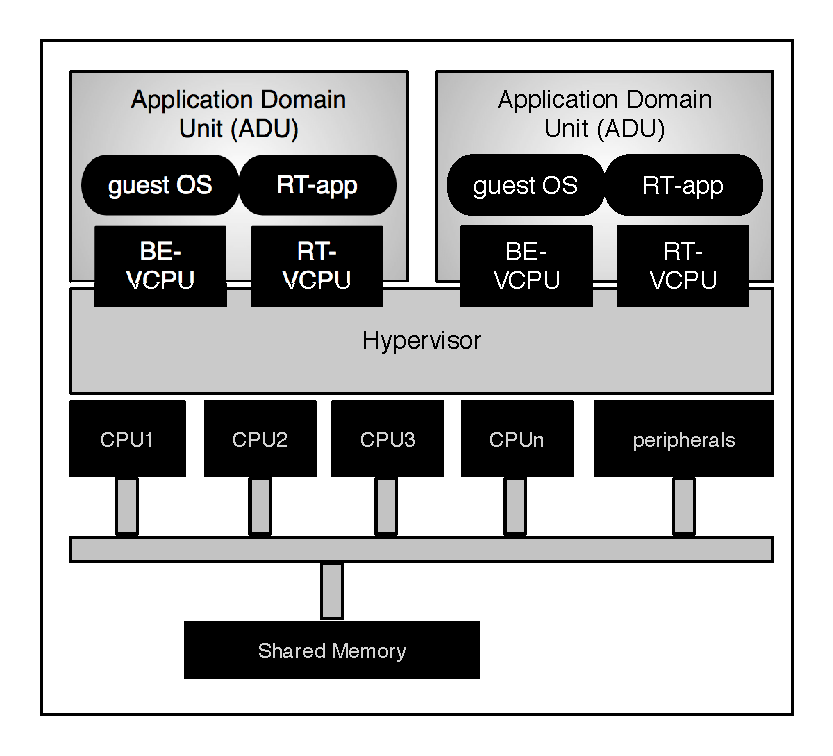
\includegraphics[width=0.50\textwidth]{./chapter4/figures/vhhModel}
\caption{Virtual Hellfire Hypervisor's virtualization model.}
\label{fig:vhhmodel}
\end{figure}

The VHH's model was designed to be compatible with the existing embedded processors that were available at the time it was developed, see Section \ref{section2:future}. Thus, the resulting model does not support essential hardware features to meet security and performance providing full-virtualization without hardware-assistance. A side effect is the absence of spatial isolation between the guest OS's kernel and user modes. Without additional processor privilege levels, the entire guest OS must execute in user-mode. In addition, all privileged instructions must be handled by the hypervisor. Thus, the model can only be used when the processor meets the Popek and Goldberg requirements (see Subsection \ref{subsection:vz-requirements}). 

Aguiar's model provides weak temporal isolation between real-time and non-real-time applications since it does not provide spatial isolation between BE-VCPUs and RT-VCPUs. Figure \ref{fig:vhhmodel} shows that BE-VCPUs and RT-VCPUs coexist in ADUs. Sharing memory space is advantageous for software stack sharing and communication performance. This means that a GPOS could instantiate RT-VCPUs that share all its software stack and communicate using shared memory. However, this approach has one major drawback. A RT-VCPU may be prevented from executing because a BE-VCPU is holding a shared lock causing a priority inversion. The model proposed in this work, implements spatial isolation between real-time and best-effort VCPUs to provide stronger temporal isolation between them.

The VHH's model was implemented in the 4Kc MIPS processor. This implementation required the modification of the target processor to allow virtualization of the MIPS's exception vector \cite{moratelli2015}. As the processor's core was modified the hypervisor could not be evaluated in a hardware platform, thus only OVSim \cite{ovp2015} simulations were performed. Also, the resulting implementation has performance issues as shown in \cite{aguiar2013}. Despite the fact that full-virtualization avoids the need for guest OS modifications, the absence of hardware-assistance forces the hypervisor to intervene constantly in the execution of the guest OS. The hypervisor handles all system interrupts routing them to the destined guest OS. VHH uses the trap-and-emulate strategy to deal with privileged instructions. Additionally, memory mapped devices use a similar strategy. When the guest OS tries to access a protected memory address, the hypervisor intervenes checking if it is a valid address to the guest OS, if so, the hypervisor proceeds to emulate the operation. The model proposed in this dissertation uses hardware-assistance to avoid excessive hypervisor intervention. Finally, guest OSs are allowed to access memory mapped devices directly and interrupts targeted to guests can be directly routed. 


\section{Final Considerations}
\label{section:final4}

The proposed embedded virtualization model was designed to take advantage of the current technologies available in the embedded processor families. These technologies allow for full-virtualization of the CPU, but they do not support efficient I/O virtualization. Despite the advantage of avoiding guest modifications, experience with the VHH has shown that full-virtualization without proper hardware support results in excessive overhead. Thus, this model avoids full-virtualization for hardware subsets without proper hardware-assisted virtualization. As a result, the proposed model implements a hybrid approach, which provides full-virtualization for the CPU and para-virtualization for I/O devices. Additionally, a list of major features for embedded virtualization was determined and the model was designed to support them. For example, spatial isolation among VMs is guarantied based on hardware support while temporal isolation is provided by BE and RT-VCPUs. Moreover, the extended services concept uses para-virtualization to allow inter-VM communication and real-time service management.

The hierarchical scheduling problem is avoided by the introduction of the RT-VM that maps real-time services directly onto RT-VCPUs. The flexible scheduling mapping proposed may cause the LHP (Subsection \ref{subsection:holder}) because a multiprocessing OS with concurrent VCPUs may be preempted while holding a spinlock. However, the LHP is not directly addressed in the model, since this problem requires different approaches depending of the scheduling algorithm implemented. But, it can be avoided with different approaches. For example, the real-time services proposed in this model does not implement spinlocks. Thus, they will not be subjected to the LHP. Additionally, single-core processors where the hypervisor maps each VM to a single VCPU does not suffer from the LHP.

The model proposed in this dissertation strengthens the hypothesis that is possible to have an embedded lightweight hypervisor capable of supporting the major embedded virtualization requisites Moreover, hardware-assisted virtualization is important to achieve low footprint and high performance. 

%hypothesis that a definition of an embedded virtualization model using hardware-assisted virtualization would result in a hypervisor capable of supporting the key required features for embedded virtualization. 


\chapter{\label{chapter:implementation}Hellfire Hypervisor - An Implementation Using MIPS Hardware-assistance}

This chapter presents a hypervisor implementation based on the virtualization model discussed in Section \ref{chapter:vtmodel}. This implementation was partially built by Zampiva \cite{samir2013} during his master degree, and finished during the development of this dissertation. Focused on full-virtualization, as proposed by the model, this implementation supports the MIPS virtualization extensions (MIPS VZ). The target processor is the M5150 that supports two-level TLBs, thus, it allows memory isolation at both the hypervisor and guest OS levels. Additionally, this chapter shows how software design decisions based on hardware-assisted virtualization associated with embedded systems characteristics result in a simpler hypervisor. Section \ref{chapter5:m5150} gives a brief description of the MIPS M5150 processor core. Section \ref{section:architecture} describes the software architecture of the hypervisor implementation. Section \ref{section5:vmm} explains the memory virtualization strategy adopted. Finally, Section \ref{section5:interrupt} describes the fast interrupt delivery mechanism supported by the hypervisor. 

\section{The M5150 processor}
\label{chapter5:m5150}

The M5150 processor was released by the end of 2013 and was one of the first cores based on the MIPS32 Release 5 (MIPS32r5) specification. It is a fully synthesizable MIPS processor designed for embedded applications. The main features of the processor are: single-core, 5-stage pipeline, 32-bit address and data paths, MIPS32 and microMIPS ISA \cite{micromipsISA}, 16 or 32 dual-entry joint Translation Lookaside Buffer (TLB) with variable page sizes, Multiply/Divide Unit, Floating Point Unit (FPU), upto 16 general purpose register shadow sets (copies of the normal GPR to avoid the need to save and restore them on entry to high-priority interrupts or exceptions) and Virtualization Module Support (MIPS VZ). Additionally, as part of the virtualization module, the core has two COP0 instances: one for the guest OS and the other exclusive to the hypervisor. Moreover, in the M5150 terminology the COP0 state for the guest OS is called guest-context while the COP0 state for the hypervisor is called root-context of the processor.

\subsection{MIPS32's Memory Model}

Figure \ref{fig:mips_memory} depicts the memory model of the MIPS32 processor family. The memory map for processors that implement TLB is different from processors with fixed mapping. For example, the M5100 processor does not implement the TLB on the guest's level. Thus, only the hypervisor has control over the virtual memory. The M5100 is designed for guests without TLB support. The MIPS-VZ module always requires the root-context TLB. For the purpose of this dissertation, only the memory model of the M5150 processor with two-stage TLB is presented. 

The MIPS32 core has 4 gigabytes (GB) of virtual memory space and supports 4GB of physical memory. The virtual memory space is divided into four segments for different purposes. The kuseg support 2GB of virtual address range and starts at 0x0000\_0000. It is designed for user applications and can be mapped through the TLB anywhere in the physical memory. The kuseg can be accessed from kernel or user-modes. The segments kseg0 and kseg1 are designed for OS's code and data. It only can be accessed from kernel-mode. Access to these segments from user-mode will cause an address error exception. Both segments are directly mapped to the lower 512 megabytes (0.5GB) of the physical memory. For example, the addresses 0x8000\_0000 and 0xA000\_0000 are mapped to the physical address 0x0000\_0000. However, the kseg1 does not support cache and is used during boot time and for memory-mapped I/O. The last two segments, kseg2 and kseg3, are accessible only in kernel-mode and can be mapped anywhere in the physical memory. These segments were intended to execute programs in supervisor mode. However, it took many years from the conception of MIPS32 before the virtualization in these processors could take place. Additionally, the Linux Kernel uses these segments as high kernel memory. 

\begin{figure}[!hbtp]
	\centering
	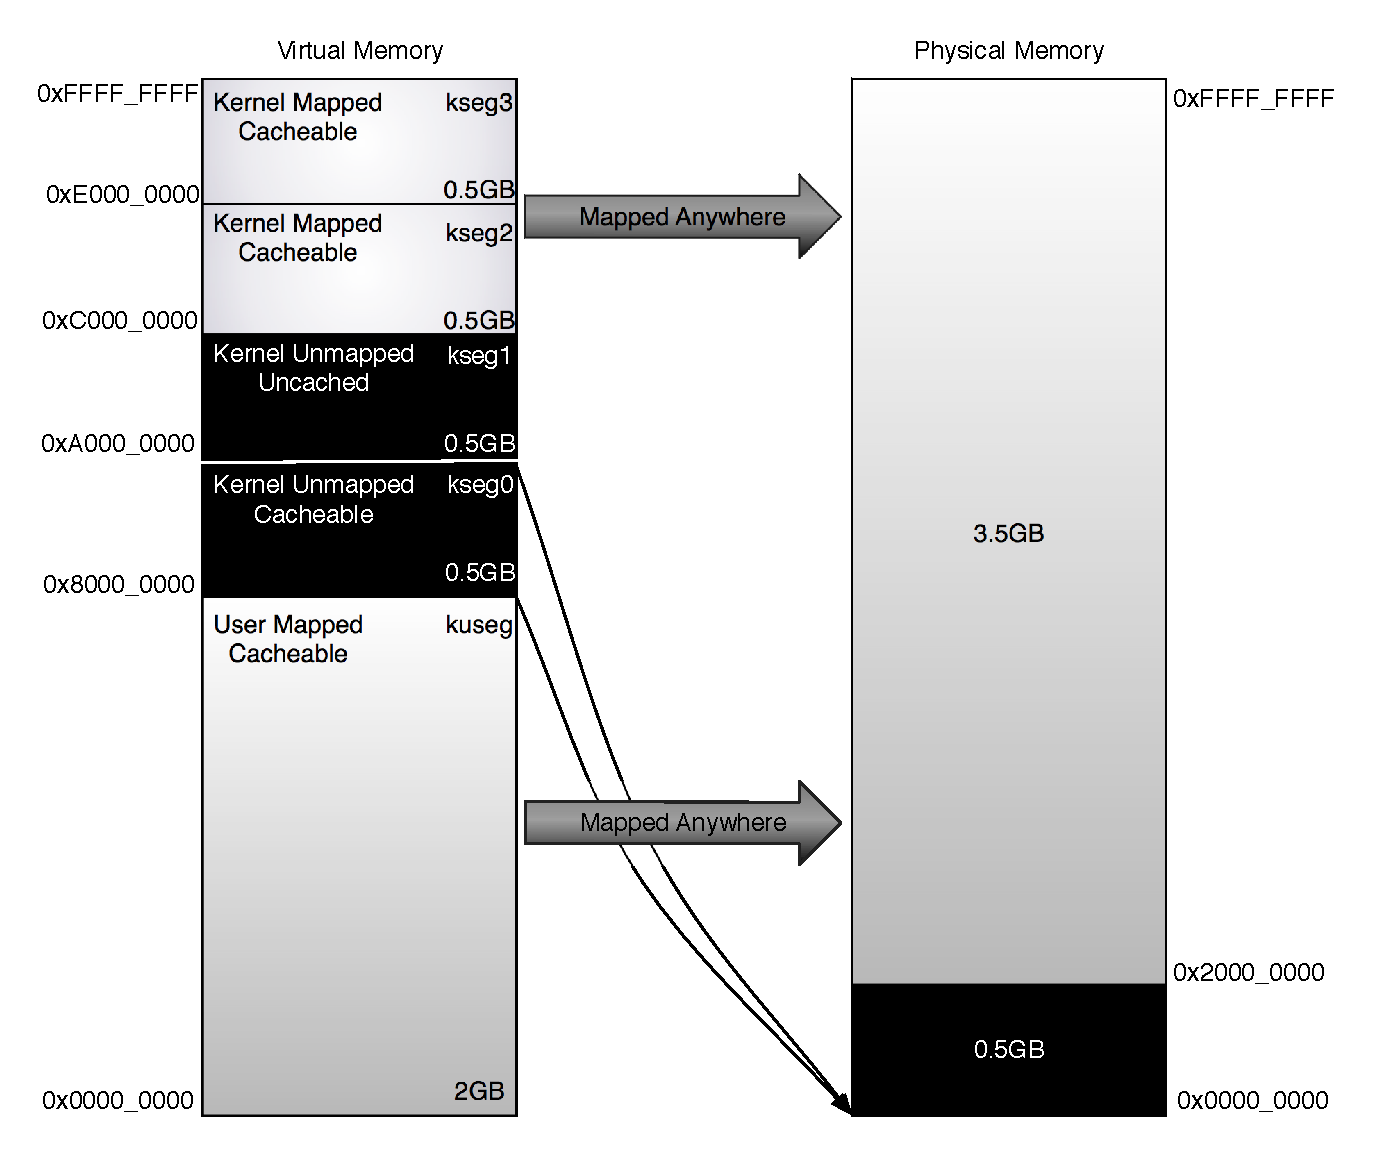
\includegraphics[width=0.5\textwidth]{chapter5/figures/mips_memory_map}
	\caption{MIPS32 memory map.}
	\label{fig:mips_memory}
\end{figure}

%\section{Hypervisor Memory Organization}


\section{Software Architecture}
\label{section:architecture}

The source code of our hypervisor was written mainly in the C programming language, but some hardware abstraction layer (HAL) parts were written in assembly. For implementation, debug and simulation purposes it was used the MIPS Instruction Accurate Simulator (IASim), which is a hardware simulator for MIPS processors able to simulate an entire platform, and based on the OVSim. However, during the development of this dissertation, only the M5150 processor, serial port and RAM memory models were available. IASim performs fast simulation aiming to deliver a virtual platform for embedded software development without the need of the real hardware platform. For better accuracy, all performance tests were performed on the SEAD-3 \cite{sead32010} development platform board, as detailed in the Chapter \ref{chapter6:evaluation}.

Figure \ref{fig:blockdiagram} shows the block diagram of hypervisor software implementation. It is composed of a hardware abstraction layer (HAL),
real-time and best-effort schedulers, dispatcher, VCPU manager, VM instantiation and toolkit. 

\begin{figure}[!hbtp]
	\centering
	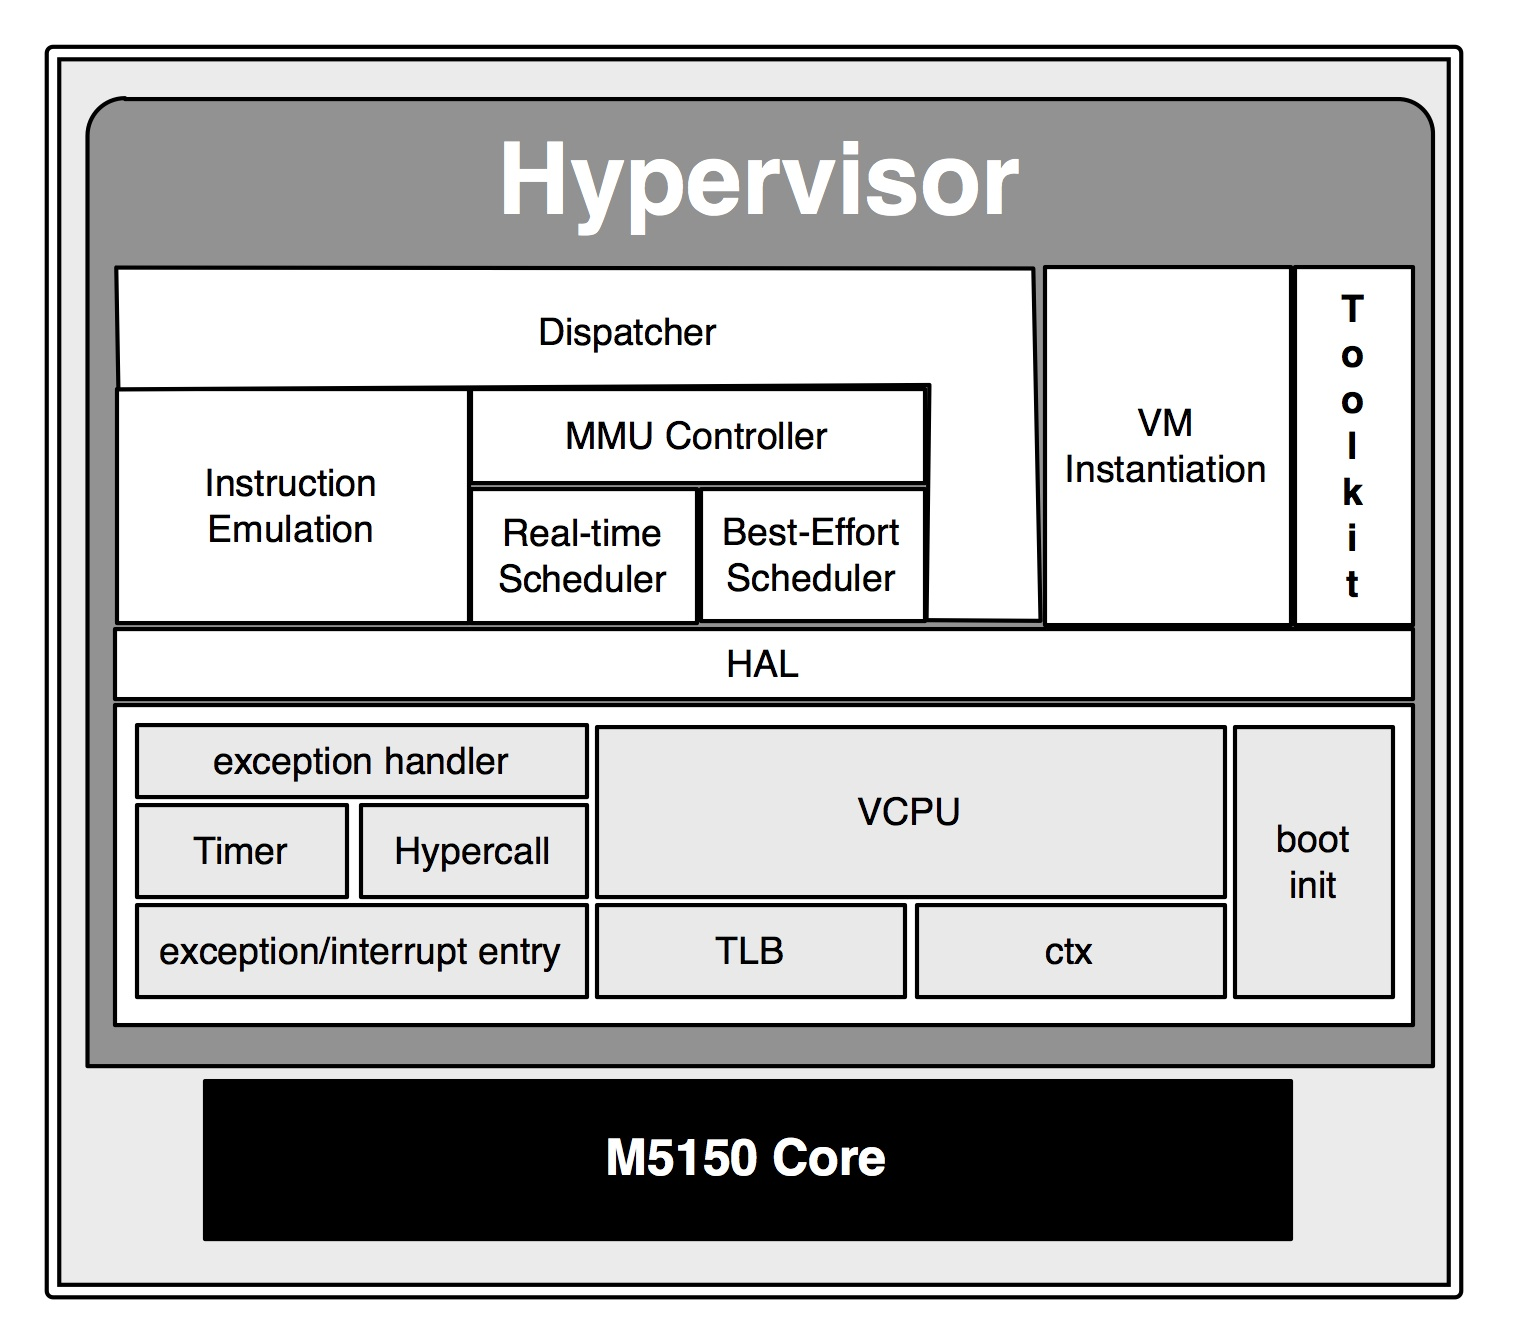
\includegraphics[width=0.5\textwidth]{chapter5/figures/hyperLayerView}
	\caption{Hypervisor's software block diagram.}
	\label{fig:blockdiagram}
\end{figure}

The HAL implements the low-level application programming interface (API) used to isolate higher layers from further hardware details. Some HAL parts were written in MIPS assembly language due to the necessity of use specific COP0 access, TLB or cache control instructions. After reset, the M5150 processor starts the instruction fetch at address 0xBFC0\_0000 in the kseg1 memory segment (non-cacheable). For a stand-alone boot process, e.g., when a boot-loader software is not present, the boot init code is placed at this address to be the first code executed after reset. This code must configure the processor accordingly and copy the hypervisor code to a cacheable memory area, in this case, the kseg0 memory segment. This boot process is used with the IASim. In the SEAD-3, the native bootloader (Yammon) is used to configure the processor and copy the hypervisor directly to the kseg0 segment. Thus, avoiding the use of the hypervisor's boot-init code. 

The real-time and best-effort schedulers are responsible for implementing the Earliest Deadline First (EDF) and best-effort round-robin scheduler algorithms for scheduling the RT-VCPUs and BE-VCPUs, respectively. The scheduler module can be easily substituted by any other algorithm. During timer interrupt handling, the hypervisor invokes the scheduler module that manages the VCPU's queues returning to the scheduled VCPU. Consequently, the dispatcher is responsible for dispatching the chosen VCPU to the physical CPU. Thus, the dispatcher uses the HAL interface to write onto the correct CPU's registers. 

The instruction emulation module is needed to emulate instructions that cannot be directly executed by the guest OS, e.g., write to specific bits of the COP0 that change the overall processor behavior as the reduced power mode bit in the status register. As a result of the MIPS-VZ module, a minimal number of instructions need to be emulated. %Subsection \ref{subsection6:impactpriv} describes the remaining instructions emulated during the boot process of the Linux and Hellfire OSs. 

The VM instantiation module is used during the hypervisor's initialization process to configure and start up the VMs. Finally, the toolkit module is a collection of software tools such as linked-list and UNIX compatible libraries. 

\subsection{Virtual Machine and Virtual CPU Software Abstraction}
\label{chapter5:vcpu_abstration}

A virtual machine must create the abstraction of a different hardware set from the original hardware platform. This different view consists of a subset of the real platform, like a compatible subset of the processor or a small amount of the entire memory. Additionally, the virtual machine can emulate hardware subsets that do not exist in the underlying hardware. KVM uses Qemu for this purposes. Pragmatically, a VM is a data structure that keeps all information necessary to control the guest execution. The VM data structure is showed in details in Appendix \ref{appendix:vm}. Typically, this data structure is kept for each guest OS. In this implementation, the VMs are allocated dynamically during the hypervisor initialization. Thus, the hypervisor's kernel uses the control information kept in these data structures to control the guest behaviors. 

Virtual CPU is an abstraction of the real CPU used to keep the last state of the CPU's registers during a context-switching. Similar to VMs, VCPUs are represented by a data structure in memory and are dynamically created during the hypervisor’s initialization. The VCPU data structure is showed in details in Appendix \ref{appendix:vcpu}. VCPUs are the execution unity of the VMs, each one represents a different execution thread. Thus, the level of concurrence in a VM depends on the number of VCPUs associated with it and the level of concurrence in the hypervisor is directly related to the total number of VCPUs in the system. There is no performance improvements if multiple VCPUs are given to a VM on a single-core processor, instead, the context-switching overhead will cause performance penalties. Thus, this implementation does not support multiple VCPUs for a VM, since the target processor is single-core. 


\section{CPU Virtualization Strategy}

The virtualization model described in the Chapter \ref{chapter:vtmodel} suggests full-virtualization of the CPU. VHH \cite{aguiar2013} implements full-virtualization of the CPU using a trap-and-emulate strategy (see Section \ref{section:vhh}) causing frequent hypervisor interventions, since all privileged instructions result in traps. This hypervisor implementation takes advantage of the hardware-assisted virtualization of the M5150 processor core. As a result, a hypervisor able to execute guest OSs with minimal intervention is expected. This section describes how the hypervisor uses the MIPS-VZ module to avoid traps. 

The MIPS-VZ module allows the hypervisor to use a different hardware configuration for each guest. Thus, the virtualized system can support software from different hardware platforms by running guests with different configurations. Additionally, the guest OSs can have features and capabilities that are different from the host processor and other guests. These different views are possible because the hypervisor can determine what processor feature subset is accessible from the guest-context. In root-context, the hypervisor configures the GuestCtl0 (guest control register 0) register that controls what privileged features can be accessed from the guest mode. 
Using the GuestCtl0 register, the designers can choose fewer hypervisor interventions, consequently less control over the processor hardware. Alternatively, they can opt for more hypervisor interventions that give them better hardware control. Some virtualized systems require more accurate hardware control, e.g., when guest OSs wish to configure different cache algorithms. In this case, the hypervisor will keep the cache instructions privileged and control the cache operation. This hypervisor implementation is focused on avoiding hypervisor interventions during guest executions as much as possible. Thus, reducing overhead and improving real-time behavior.  Table \ref{table5:guestctl0} summarizes the configurable processor features.  First, the hypervisor gives general access to the coprocessor 0 (CP0) using the bit 28 of the GuestCtl0 register. However, some features in the CP0 remain privileged. Thus, the hypervisor allows access to the cache instructions, setting the CG field (bit 24), which allows the guest to configure the cache algorithms. Still, guest OSs are allowed to have access to the config 0 through config 7 registers. The config register set specifies various configuration and capability information. Most of the fields in the config registers are initialized by hardware during the exception reset process, or they have constant values \cite{m5150}. When the hypervisor wishes to give a different view of the system configuration to a certain guest OS, it must keep the config registers privileged. Thus, reads to this registers in a guest-context will trap the hypervisor that performs a trap-and-emulate strategy. The config registers are unprivileged in guest-context when the bit 23 of the GuestCtl0 register is set. Finally, the guest OSs can directly access  the timer registers. Timer virtualization is explained in Subsection \ref{subsection5:timervz}.

\begin{table}[!hbtp]
\centering
\caption{GuestClt0 register fields. These bits are used to control the hardware accessibility by the guest OS.}
\label{table5:guestctl0}
\begin{tabular}{lll}
\hline
\hline
\multicolumn{2}{c}{\textbf{Fields}}                                   & \multicolumn{1}{c}{\multirow{2}{*}{\textbf{Description}}} \\ %\cline{1-2}
\multicolumn{1}{c}{\textbf{Name}} & \multicolumn{1}{c}{\textbf{bits}} & \multicolumn{1}{c}{}                                      \\ \hline 
CP0                               & 28                                & Guest access to coprocessor 0.                            \\
AT                                & 26-27                             & Guest Address Translation control.                        \\
GT                                & 25                                & Guest Timer register access.                              \\
CG                                & 24                                & Cache Instruction Guest-mode enable.                      \\
CF                                & 23                                & Config register access.                                   \\ \hline
\end{tabular}
\end{table}


Despite the MIPS-VZ module support, some registers or specific bits of the registers always remain privileged. For example, the reduced power mode bit in the status register will always trap the hypervisor on guest write attempts. A VM should not have direct control of the processor performance or any other feature that could disrupt the execution of other VMs. Another reason to keep certain registers privileged is to give a different view of the system to a certain guest OS, as performed by the config registers. The same case applies to the processor identification (PID) register. When the guest OS is trying to identify the processor, the hypervisor can return a different processor identification. For example, in the M5150 processor the hypervisor can return the 4Kc processor identification limiting the guest to a compatible processor subset. %Subsection \ref{subsection6:impactpriv} presents the impact performance results for the remaining privileged instructions.

The hypervisor can keep different views of the hardware to different VMs modifying the desired fields of the GuestCtl0 register during context-switching. Thus, the only hypervisor requirement is to keep an individual copy of the GuestCtl0 register in the VM's software control structure for each guest OS. This hypervisor implementation keeps direct access to all features described in Table \ref{table5:guestctl0}. 


\subsection{Best-effort and real-time scheduler algorithms}
\label{subsection:best-effort-edf}

The hypervisor implements both Earliest Deadline First (EDF) ~\cite{edf} and best-effort (round-robin) policies to deal with RT-VCPUs and BE-VCPUs, respectively. The EDF has higher execution priority than the best-effort scheduler. The latter  will not suffer from starvation since the implementation counts on time reservation for it. The EDF scheduler requires the deadline (D), period (P), and capacity (C) real-time parameters, which are received from the hypercall HCALL\_RT\_CREATE\_APP, as explained in Section \ref{subsection4:services}. For the sake of simplicity, BE-VCPUs and RT-VCPUs are kept in different software queues.

\begin{figure}[!hbtp]
	\centering
	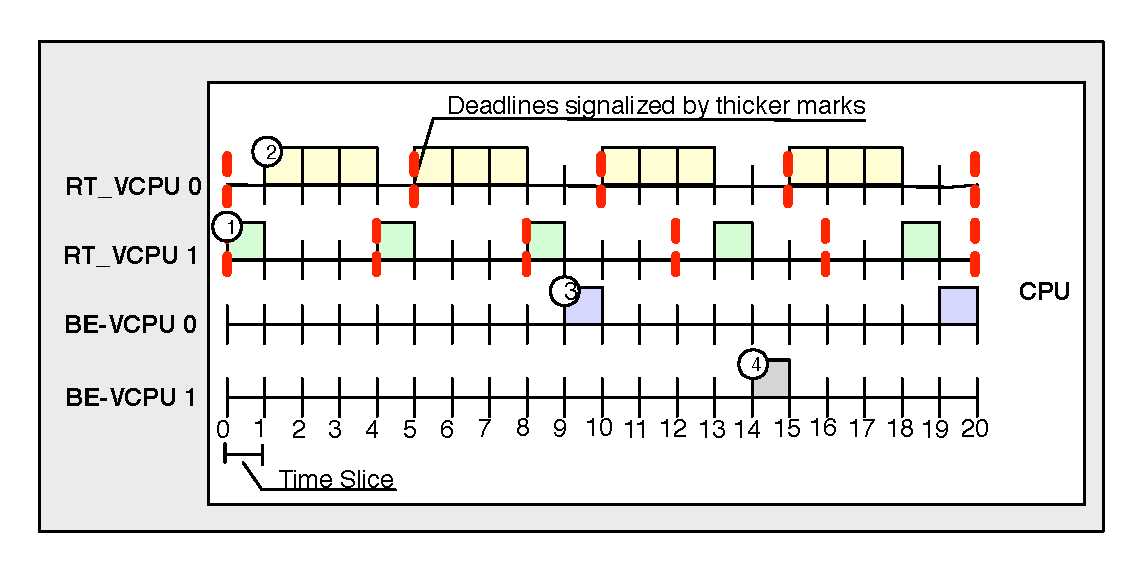
\includegraphics[width=0.7\textwidth]{chapter5/figures/tasks_scheduler_line}
	\caption{Example of the scheduling strategy to combine the EDF and best-effort schedulers.}
	\label{fig5:task_scheduler_line}
	\vspace{-0.5cm}
\end{figure}


Figure \ref{fig5:task_scheduler_line} illustrates the scheduling strategy where both EDF and best-effort schedulers cooperate to increase the CPU utilization. Assuming the execution of two BE-VCPUs and two RT-VCPUs with the following real-time parameters:

\begin{itemize}
    \item RT-VCPU 0: period = 5, capacity = 3 and deadline = 5;
    \item RT-VCPU 1: period = 4, capacity = 1 and deadline = 4.
\end{itemize}

The BE-VCPUs have the same priority. The scheduling scenario during 20 time slices can be viewed in Figure \ref{fig5:task_scheduler_line}. Each RT-VCPU is scheduled according to the EDF policy. Thus, RT-VCPU 1 executes in the first quantum as shown in (1). Next the RT-VCPU 2 executes three quanta, according to (2). In quantum 9, BE-VCPU 0 is executed for the first time because there was not any RT-VCPU ready to execute in this time slice (see (3)). Finally, The BE-VCPU 1 is executed for the first time on quantum 14 according to (4). Thus, when executed concurrently, BE-VCPUs will only execute when the RT-VCPUs are not ready to execute. An amount of CPU time can be reserved for best-effort VMs to avoid starvation. The schedulability test for the EDF algorithm when the deadline is equal to the period is determined by the following equation:

\begin{equation}
\label{eq5:schedulability}
\displaystyle U = \sum_{i=1}^{n} \frac{C_i}{P_i} \leq 1
\end{equation}

U is the CPU utilization. Thus, the sum of the ratios between the capacity and the period of all real-time tasks must be less than 1. The equation \ref{eq5:schedulability} can be used to reserve an amount of CPU for best-effort tasks. For example, if the designers wants to reserve at least 40\% of the CPU time for the best-effort, the result of the above equation must be less than to 0.6, according to equation \ref{eq5:schedulability}. Note that the amount of CPU dedicated to real-time and best-effort tasks is determined at design time. However, during the creation of RT-VCPUs the hypervisor checks the amount of CPU used and if it exceeds the maximum time allowed it will not be created. 

%explicar como essa questão ficou na implementação (quando a vcpu não é criada).


\subsection{Timer Virtualization}
\label{subsection5:timervz}
\vspace{-1cm}

Timer virtualization is an important topic for hypervisor implementation, since it implements the timing view from the VM's perspective. MIPS32 cores can be configured to generate timer interrupts periodically. Two registers are used to configure the timer: counter and compare registers. The counter is incremented for each other processor's clock. When the counter value is equal to the compare register, the processor's core generates a timer interrupt. Thus, the hypervisor or OS that wants to generate timer interrupts must read the counter value, add the amount of time to the next interrupt and write the resulting value to the compare register. This procedure must be performed on each timer interrupt to keep its periodicity. 

The accessibility of the compare and timer registers from the guest-context is controlled by the GT field on the GuestCtl0 register. Allowing direct access to the counter and compare registers, the guest OS will be able to perform read and writes to the compare register and reads to the counter registers. Thus, the guest OS cannot perform writes to the counter, since it will disrupt the global view of the system timer. In fact, a typical OS implementation will write on the counter register only during its initialization. Therefore, the hypervisor needs to emulate a few writes to the counter register during the VM's initialization. This hypervisor implementation allows the guest OSs direct access to the timer registers avoiding traps during context-switching of the guests. 

The hypervisor implements timekeeping within VMs, i.e., it can decide what to do with the time frame that a VM was not executing. The guest OS's time view is called virtual time. The MIPS-VZ module has a special register to configure the time within VMs called GTOffset. This register accepts a two's complement value that will add or subtract the current value of the counter in the guest-context. Thus, the hypervisor can hide the time frame that the VMs were not executing. However, this implementation gives an absolute time view to the guest OSs, i.e., they are aware of the lost time frames. Thus, the value written to the GTOffset is zero, resulting in a virtual time equal to the absolute time. 


% talvez falar da implicação disso em escalonamento hierarquico. 


\section{Virtual Memory Management}
\label{section5:vmm}


The MIPS VZ module implements a second-stage TLB translation in the hardware. Essentially, the hardware performs the translation from IPA to PA without software intervention, as explained in Subsection \ref{subsection:hardware-assisted}.  The hypervisor still manages its page table mapping IPA to PA in a second-stage TLB. The guest OS is allowed to configure directly the first-stage TLB. The resulting PA is generated by the hardware combining both TLBs. This mechanism decreases the number of hypervisor exceptions drastically and also hypervisor complexity. The M5150's TLB supports a second-stage TLB translation and a range of page sizes from 1Kbyte to 256Mbytes. Our hypervisor takes advantage of large pages to avoid TLB misses during IPA to PA translations. VMs are loaded into a contiguous memory region, and the IPA translation is statically mapped to reserved TLB entries. For example, to allocate 32Mbytes of physical address space to a VM, the hypervisor uses a dual-TLB entry (MIPS' TLB allows to map two pages by TLB entry) to map two consecutive 16Mbyte pages in the second-stage TLB. Figure \ref{fig:tlb-hyper} depicts this scheme. The guest OS manages the first stage address translation in exactly the same way as on a non-virtualized system. In the second-stage translation, the hypervisor maps a virtual memory address range to a contiguous physical address range.

\begin{figure}[!hbtp]
	\centering
	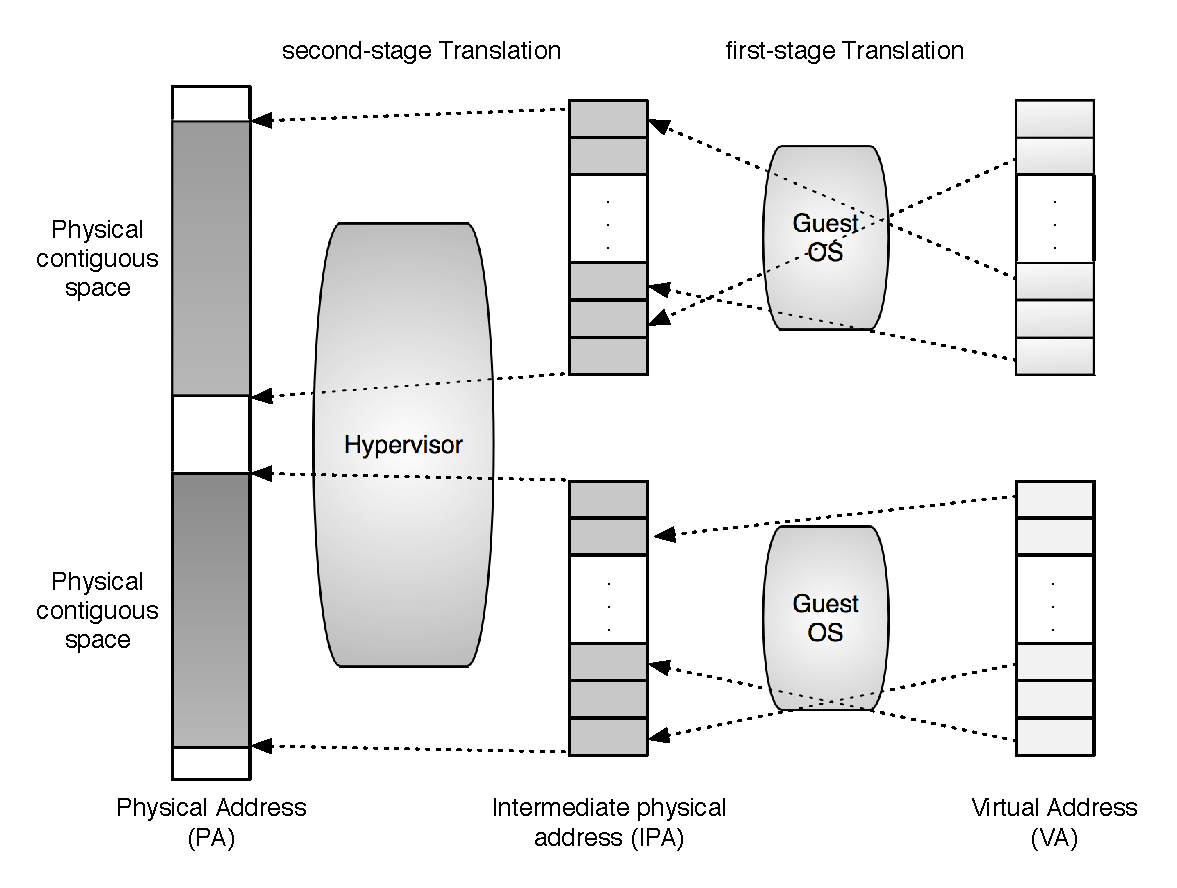
\includegraphics[width=0.6\textwidth]{chapter5/figures/tlb-hyper2}
	\caption{Virtual memory organization view of our hypervisor.}
	\label{fig:tlb-hyper}
\end{figure}


Typical hypervisors for cloud computing implement a complete paging mechanism. The hypervisor keeps a page table to map guest OSs to physical addresses. In these systems, the guest OS does not need to be entirely loaded into the main memory to be executed. In fact,  the hypervisor can implement an on-demand paging mechanism (swapping). Such a scheme reduces the memory usage since pages that have not been used recently can be stored in the swapping system. Additionally, it avoids the memory external fragmentation problem because the VMs do not need to be allocated contiguously in the physical memory. However, this approach has critical drawbacks for ESs. First of all, swapping systems and on-demand paging mechanisms impact real-time responsiveness. Additionally, some ESs do not support swapping due to storage restrictions. Moreover, a complete virtual memory management mechanism implies a more complex hypervisor and, consequently, a larger footprint and more processing requirements. 

A simplified virtual memory management mechanism brings some advantages to ESs. First, it avoids second-stage TLB misses keeping the VM entirely mapped at the TLB during its execution. Thus, RTOSs that do not implement virtual memory support will not suffer additional delays and jitter due to hypervisor paging management. Secondly, some ESs execute a limited number of virtual machines and some keep a static configuration during their execution. For these systems, memory fragmentation due to contiguous guest OS allocation is not a major problem. This implementation supports mapped devices directly, i.e., it can map non-continuous memory regions to a VM. Usually, such devices are mapped to specific physical addresses requiring a special mapping for guest access. For example, a VM may have mapped 32Mbytes of RAM to be loaded into the physical memory at 0x1000\_0000. If the same guest requires access to a memory mapped peripheral at physical address 0x1F00\_0800 the hypervisor must configure a second-stage TLB entry to match this address. Finally, a VM requires, at least, one TLB-entry to be mapped at the second-stage TLB, and an additional TLB-entry for each directly mapped peripheral. The M5150 has 32 TLB-entries. If the number of TLB-entries needed to map all VMs and peripheral on a system exceeds 32 entries, the hypervisor must reconfigure the TLB on each context-switching.  

\section{Interrupt Virtualization}
\label{section5:interrupt}

The MIPS VZ module allows to map an interrupt source directly to a guest OS avoiding hypervisor intervention. This mechanism is known as interrupt pass-through and it allows one to support directly mapped devices. Therefore, it does not share devices between guests, but allows a certain guest OS to have direct access. The main advantage of this technique is low overhead, which is close to non-virtualized systems in terms of throughput and latency. However, if an  interrupt occurs during the execution of any other guest OS, the hypervisor must decide between:

\begin{itemize}
    \item keep the interrupt masked and delay its delivery or;
    \item intercept the interrupt and reschedule the guest OSs.
\end{itemize}

This allows the implementation of different policies for interrupt control. For example, for low priority devices such as a serial port for a user console, the hypervisor may choose to keep the interrupt masked while in the supervisor mode. Thus, the guest OS will handle the interrupt only on its next execution (hypervisor scheduling quantum), resulting in a relatively long delay. This requires a large buffer queue in hardware or hardware flow control, otherwise, data may be lost. This arrangement is acceptable for low bandwidth, non interactive devices. Devices with higher priority or higher bandwidth may require hypervisor intervention to avoid long delays in the interrupt handling. To illustrate a typical scenario, suppose that a Linux guest has a directly mapped Ethernet device.  In this case, the hypervisor can keep the Ethernet interrupt unmasked to perform a context switch between guests when a network packet is received and the Linux guest is not executing.

\begin{figure}[!hbtp]
\centering
\subfigure[Interrupt delayed.]{
    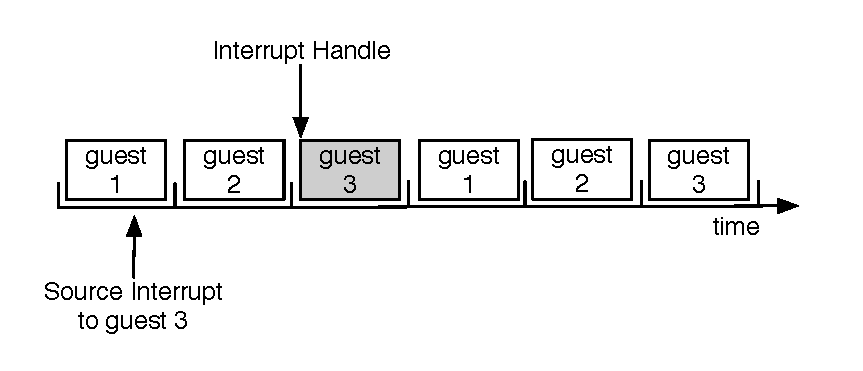
\includegraphics[width=.4\textwidth]{chapter5/figures/interruptdelay}
    \label{subfig:interruptdelayA}
}
\subfigure[Fast interrupt with recycled quantum.]{
    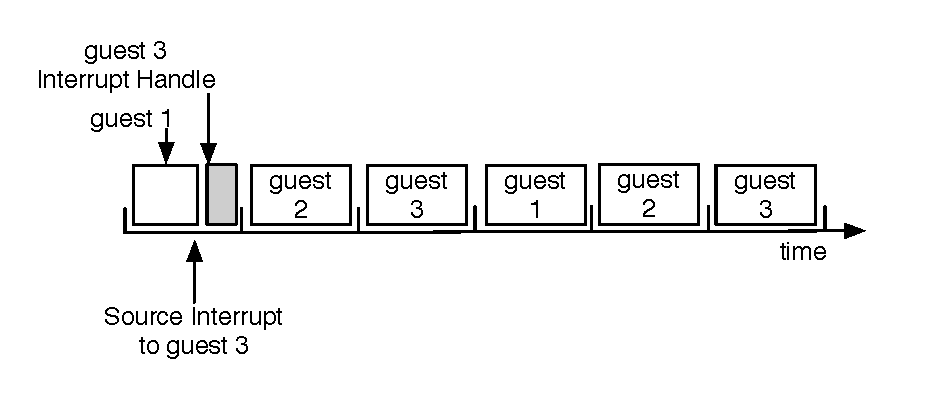
\includegraphics[width=.4\textwidth]{chapter5/figures/interrupt_short_quantum}
    \label{subfig:interruptdelayB}
}
\subfigure[Fast interrupt with reset quantum.]{
    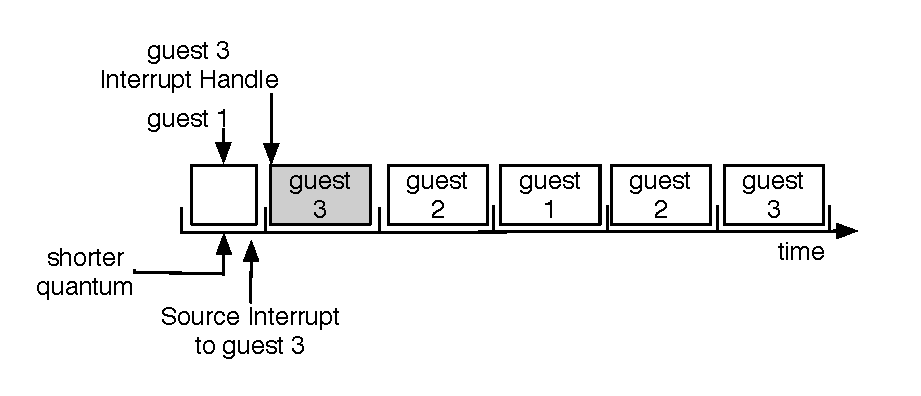
\includegraphics[width=.4\textwidth]{chapter5/figures/interrupt_new_quantum}
    \label{subfig:interruptdelayC}
}
\captionsetup{justification=centering}
\caption{Quantum scheduler scheme for interrupt delivery.}
\label{fig:interruptdelay}
\end{figure}


Figure \ref{fig:interruptdelay} depicts three guest OSs being scheduled in a round-robin policy with the three different quantum schemes for interrupt handling. Figure \ref{subfig:interruptdelayA} shows an interrupt targeted to the guest OS 3 being asserted during the execution of the guest OS 1. Without a proper hypervisor policy, the interrupt delivery will be delayed until the execution of the guest OS 3. In fact, the overhead is similar to a non-virtualized system since there is no hypervisor intervention. However, this causes a long delay to deliver the interrupt. This implementation was designed to use the interrupt pass-through mechanism, which allows for the coexistence of general-purpose OSs and RTOSs with minimal interrupt delivery delay. First, we studied two different schemes regarding the use of the scheduler quantum: recycle quantum and reset quantum. Figure \ref{subfig:interruptdelayB} shows a fast interrupt delivery approach, causing the preemption of the current guest OS and the dispatch of the guest which will execute during the time remaining in the same quantum. In Figure \ref{subfig:interruptdelayC}, the current quantum is shortened, and the dispatched guest will execute during an entire new quantum. Chapter \ref{section6:interruption-delay} presents the results and discussion about the implications of these different approaches. 

Independently of the quantum scheme adopted, our hypervisor accepts a set of rules to describe the behavior to address different interrupt sources. This set of rules is defined at design time. For each guest OS, the designers define which interrupts are directly mapped and, if an interrupt can induce the preemption of the current guest OS. Additionally, a higher priority guest OS can be marked to never be preempted by the hypervisor during its scheduler quantum. Table \ref{table:rules} shows a possible configuration for three guest OSs. Guest 1 has the timer and serial 1 interrupts directly mapped. The column Root Int describes which interrupts will trigger the hypervisor when the guest is not executing. In this case, the hypervisor will intercept serial 1, dispatching Guest 1. Guest 2 has the timer and serial 2 interrupt sources directly mapped. The hypervisor will intercept serial 2 interrupts when the guest is not executing only if the current guest is marked to be preempted. In the example, the hypervisor will preempt guest Linux 1 to deliver network interrupts to guest 2, but the same interrupts will be delayed if the guest 1 is executing. Thus, a high priority guest OS cannot be preempted by events from other guests, but only by the hypervisor scheduler. Our hypervisor provides a strong temporal isolation between guests, which is essential in ES virtualization if predictability of the RTOSs is a major concern. In addition, the flexibility of this approach allows the system to be configured for specific applications. Finally, our hypervisor always keeps the guest timer interrupt directly mapped, since it avoids hypervisor intervention during guest scheduling. 

\begin{table}[!hbtp]
\caption{Example of a set of interrupt rules for a system configured with three guest OSs.}
\label{table:rules}
\centering
\begin{tabular}{llll}
\hline
                                    &                                                       & \multicolumn{2}{c}{\textbf{Rules}}                                           \\ 
\multicolumn{1}{c}{\textbf{Guests}} & \multicolumn{1}{c}{\textbf{Direct Mapped Interrupts}} & \multicolumn{1}{c}{\textbf{Root Int}} & \multicolumn{1}{c}{\textbf{Preempt}} \\ \hline
Guest 1                               & Timer, Serial 1                                       & Serial 1                              & No                                   \\
Guest 2                              & Timer, Serial 2                                               & Serial 2                                  & Yes                                    \\
Guest 3                              & Timer, Network                               & Network                               & Yes                                    \\ \hline
\end{tabular}
\end{table}


\subsection{Virtual Interrupt}
\label{section5:virtual_interrupt}

The M5150 processor core supports an interrupt injection mechanism called virtual interrupt. Virtual interrupts are software generated and used when the hypervisor needs to inject interrupts in the guest OSs. Our hypervisor implements a secure inter-VM message passing mechanism described in Section \ref{chapter5:inter-vm} based on para-virtualization and virtual interrupt injection. 

%Descrever brevemente o mecanismo de injecao de interrupção.

\section{Inter-VM Communication}
\label{chapter5:inter-vm}

As explained in Subsection \ref{subsection4:comm}, the proposed virtualization model does not define a communication mechanism. However, it defines a hypercall interface for communication among VMs. Thus, this implementation adopts a message passing mechanism based on para-virtualization.  The hypervisor uses the VM identification number to route the messages among the VMs. The hypervisor requires the address, size and ID destination to route a message, which are discovered during the hypercall. Thus, the hypervisor does not make any assumptions about the message formatting; this is entirely the responsibility of the communicating guest OSs. For example, if a multi-task guest OS needs to demultiplex \cite{tanenbaum2011} incoming messages among different tasks, it may add a header to the message indicating the origin and destination task id. In this case, different guest OSs must agree about the header format.

\begin{figure}[!hbtp]
	\centering
	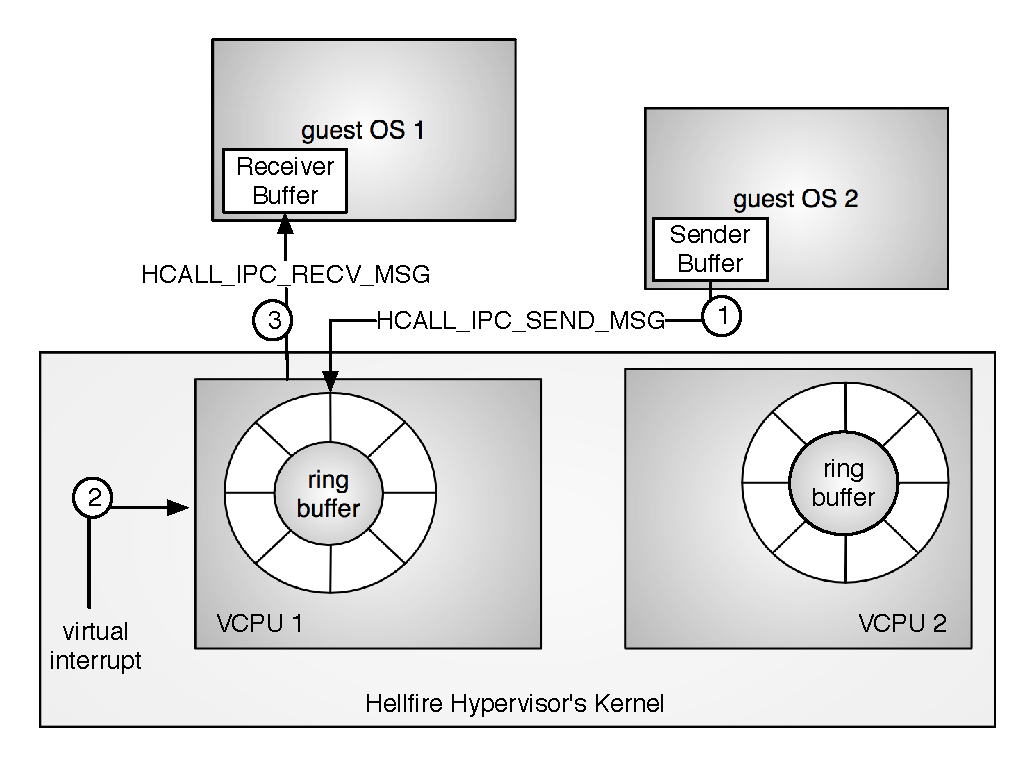
\includegraphics[width=0.5\textwidth]{chapter5/figures/intervm-comm}
	\caption{Example of inter-VM communication involving two guests.}
	\label{fig:intervm-comm}
\end{figure}

Each VCPU implements its incoming message queue as a circular buffer, statically allocated for performance purposes. A message targeting a determined VCPU will be copied to its queue, and the hypervisor will insert a virtual interrupt to the VCPU. The next time that the VCPU is executed it will handle the virtual interrupt and call the hypercall to retrieve the message. Figure \ref{fig:intervm-comm} describes the hypervisor behavior while redirecting messages between guests. The guest OS 2 invokes the HCALL\_IPC\_SEND\_MSG hypercall (1) causing a message copy from the guest's buffer to the ring buffer of the VCPU 1. After, the hypervisor injects a virtual interrupt (2) in the VCPU 1. In the next execution, the guest OS 1 will answer to the interrupt and executes the HCALL\_IPC\_RECV\_MSG hypercall. Thus, the hypervisor will copy the message from the ring buffer to the target buffer (3). 


\section{Engineering Effort to Support a Guest OS}

Due to the full-virtualization feature, to port a new guest OS to the Hellfire Hypervisor does not require any modification of the guest OS's kernel. However, it is important to highlight that the OS must be ported to the target platform. Thus, it must be able to execute natively on the hardware platform. To port an OS to a new processor or platform is a different job, and it is not necessarily related to virtualization. Thus, the designers must know some details about the memory mapping and platform resources required by the target OS. A guest OS requires specific memory regions, and it may depend on platform resources such as timer counters or other sources of interrupts. The hypervisor allows one to  describe the memory arrangement for each guest OS at design time. This description consists of mapping from IPA to PA (see Subsection \ref{subsection:hardware-assisted}) addresses that are written to the second-stage TLB by the hypervisor. The designers must choose the amount of main memory available to the guest OS based on the application and OS requirements. For example, 16MB of DRAM are enough to execute a minimal Linux distribution, while 64KB of DRAM are sufficient for a Hellfire OS guest with several tasks. Next, the designers must choose a contiguous area of physical memory to allocate to the guest OS. Additionally, the designers must determine which interrupts and peripherals will be directly mapped to the guest OS. Again, the arrangement between the source of interrupts and target guest OSs is described in a data structure at design time. In any case, the timer interrupt must at least be mapped to the guest OS, since this implementation does not provide timer emulation, i.e., each guest OS must receive its timer interrupts directly. Table \ref{table:rules} shows how the interrupt mapping can be described. 

\begin{table}[!hbtp]
\centering
\caption{Example of memory mapping for a Linux and a HellfireOS guests.}
\label{table:guestaddresses}
\begin{tabular}{
>{\columncolor[HTML]{FFFFFF}}l 
>{\columncolor[HTML]{FFFFFF}}l 
>{\columncolor[HTML]{FFFFFF}}l 
>{\columncolor[HTML]{FFFFFF}}l }
\hline \hline
                                                              & \multicolumn{3}{c}{\cellcolor[HTML]{FFFFFF}\textbf{Addresses}}                                                                                                               \\
                                                              & \multicolumn{1}{c}{\cellcolor[HTML]{FFFFFF}\textbf{VA}} & \multicolumn{1}{c}{\cellcolor[HTML]{FFFFFF}\textbf{IPA}} & \multicolumn{1}{c}{\cellcolor[HTML]{FFFFFF}\textbf{PA}} \\ \hline
\cellcolor[HTML]{FFFFFF}                                      & 0x8000\_0000                                            & 0x0000\_0000                                             & \textbf{0x1000\_0000}                                   \\
\multirow{-2}{*}{\cellcolor[HTML]{FFFFFF}\textbf{Linux}}      & 0xBF00\_0000                                            & 0x1F00\_0000                                             & 0x1F00\_0000                                            \\
\cellcolor[HTML]{FFFFFF}                                      & 0x8000\_0000                                            & 0x0000\_0000                                             & \textbf{0x1200\_0000}                                   \\
\multirow{-2}{*}{\cellcolor[HTML]{FFFFFF}\textbf{HellfireOS}} & 0xBF00\_0000                                            & 0x1F00\_0000                                             & 0x1F00\_0000                                            \\ \hline
\end{tabular}
\end{table}

Table \ref{table:guestaddresses} shows a valid memory mapping for a Linux and Hellfire OS guest. Both OSs are compiled to execute at the 0x8000\_0000 VA. Additionally, each OS require access to peripherals. Thus, a 4KB page is mapped at 0xBF00\_0000, where the peripherals mapping starts in the SEAD-3 development board (see Section \ref{section6:devboard}). Note that each guest requires, at least two TLB entries. The addresses 0x8000\_0000 and 0xA000\_0000 (including 0xBF00\_0000) correspond to the Kseg0 and Kseg1 memory segments, respectively, as shown in Figure \ref{fig:mips_memory}. These segments are fixed mapped and correspond to the 0x0000\_0000 physical address. However, when implementing the MIPS-VZ module, these addresses become IPA, and the hypervisor must map them to the PA. The PA column shows the 0x1000\_0000 and 0x1200\_0000 addresses highlighted since they correspond to the physical addresses where the guests are located in the memory. Additionally, for peripheral mapping the IPA and PA are the same because the hypervisor keeps the original addresses where the guest OSs expect to find the peripherals. 


\subsection{Linux and Hellfire OSs as Guests}

Most of the work to port an OS to the Hellfire Hypervisor is described in Tables \ref{table:rules} and \ref{table:guestaddresses}. However, some details must still be explained. Current Linux releases do not use periodic timer interrupts. In fact, when the OS is idle, it programs the timer interrupt to the next event, even if it will take several scheduler quanta, and executes the \textit{wait} instruction. This instruction will put the processor in the power saving mode. The processor comes up once an interrupt arrives. However, wait is a privileged instruction that must be emulated by the hypervisor. Emulating this instruction means to check when the next OS timer interrupt is programmed to happen and to program an event in the hypervisor to insert a virtual interrupt in the guest. However, the current implementation does not support emulation of this instruction. Thus, the Linux kernel was configured to use the periodic timer interrupt technique. Note that this is not an OS modification, since it was not needed to write kernel patches. Instead, both ways to use the timer interrupts are kernel features and they can be selected during kernel initialization. Finally, modifications were made to the Linux kernel to improve its performance once executed as a guest. This is better explained in Section \ref{section6:linuxport}.

Hellfire OS has fewer restrictions than Linux when virtualized since it is a simpler operating system. However, an initial port to the M5150 processor had to be done before it was virtualized. Once virtualized, para-virtualized communication drivers were then implemented to allow inter-VM communication. 

%The only board peripheral supported is the serial port used for communication.

\section{Current Hypervisor Restrictions}

Similar to any other implementation based on a theoretical model, the proposed hypervisor faces some limitations. The first limitation is that the M5150 is a single-core processor. The model proposes to support homogeneous multicore processors. The decision for this processor core was based on availability. The M5150 was one of the first MIPS processors, released in early 2013, implementing the MIPS-VZ technology. Additionally, it was the first MIPS core supporting MIPS-VZ module available to the GSE group. As a single-core processor, mutex or spinlocks are not required in the hypervisor since there are no concurrent executions on its kernel. A consequence is a simpler hypervisor kernel. Finally, it is important to highlight that this is a limitation imposed by the hardware platform that can be overcome when multicore processors become available.

Despite the overhead imposed by share devices, they are important in different situations. Because many guest OSs may require communication with the external world, the only solution is to implement a switching layer at the hypervisor level and para-virtualized device drivers to the VMs. The current stage of this implementation does not support any shared device, e.g. Ethernet. However, the implementation of a shared device is a matter of engineering effort since the para-virtualized interface between guest OSs and the hypervisor is already supported for inter-VM communication. The optimization and techniques to support shared devices is a future work.

The inter-VM communication implemented as a message passing mechanism is a secure and effective communication channel. However, as shown in Section \ref{subsection:intervm}, it imposes an excessive overhead to the system. Significant improvements can be achieved using a shared memory communication mechanism that is not available at this moment. 

The RT-VM concept provides strong temporal isolation among VMs. Additionally, it avoids the hierarchical scheduling problem. A restriction of the RT-VM is that it does not provide a compatible software environment for legacy software libraries. This means, any implementation must be build from scratch, impacting time-to-market and costs. However, this is a model restriction since it does not provide any tool or resource to avoid the problem. A practical implementation may avoid this problem porting a RTOS to execute as a guest in the RT-VM with its scheduler disabled, consequently, executing just one task. Thus, the application can use the RTOS's legacy libraries, but without concurrent tasks. 

The Hellfire Hypervisor was built from scratch avoiding any proprietary or open-source external library which makes it the propriety of the GSE group. However, this results in an important drawback: all engineering efforts must be from the university group. Different from several other open-source hypervisors those count on contributions from different groups, the Hellfire Hypervisor is entirely the responsibility of the GSE group. As a result, the current implementation only supports  Linux/MIPS and Hellfire RTOS guests. Additionally, there are limitations caused by the lack of engineering efforts because of  the small number of engineers working on the project. However, the Hellfire Hypervisor is planned to be released as an open-source software in early 2016. 

%1 linux guest

\section{Final Considerations}

An important question about theoretical models is how practical is it for them to be implemented on a hardware/software platform. This implementation demonstrated that the model can be implemented with relatively simple algorithms and data structures help to keep a small footprint. A factor that contributed to the simplification of the hypervisor was the M5150's hardware-assisted virtualization, especially the support for memory and MIPS CP0 virtualization. The footprint and performance results are analyzed in Chapter \ref{chapter6:evaluation}. The only feature not implemented was the multi-core support because the target processor is single-core. The absence of multi-core support simplified the hypervisor's kernel because it avoided the need for mutex or spinlocks. Other restrictions, like the lack of shared devices, concerns to the limited time and number of engineers working on the project, which can be overcome with more engineering effort. It is fair to conclude that the presented implementation is a suitable representation of the virtualization model proposed in the Chapter \ref{chapter:vtmodel}.




































\chapter{\label{chapter6:evaluation}Hypervisor Evaluation and Practical Results}

This chapter is dedicated to the evaluation of the Hellfire Hypervisor. The chapter is composed of a sequence of experiments that show the practical results for different hypervisor aspects. When possible, the results are compared to other hypervisors. Section \ref{section6:devboard} describes the SEAD-3 development board used for the hypervisor deployment. Section \ref{section6:footprint} shows the hypervisor memory footprint. Section \ref{section6:linuxport} describes the Linux/MIPS port to the hypervisor and a modification for better performance. Section \ref{section6:overhead} describes the overhead impact of the virtualization layer on the Linux/MIPS. Section \ref{section:hellfireOverhead} analyses the overhead impact of the hypervisor on the HellfireOS. Section \ref{section6:interruption-delay} evaluates the proposed fast interrupt delivery mechanism. Section \ref{subsection:intervm} shows the results of the inter-VM communication mechanism. Section \ref{section6:realtimeservices} describes two experiments to show the effectiveness of the real-time services. Finally, Section \ref{section6:finalcons} presents the final considerations of this chapter. 

\section{SEAD-3 Development Board}
\label{section6:devboard}

The SEAD-3 development platform board \cite{sead32010} was used to validate and conduct performance tests. It supports MIPS processors allowing the user to evaluate the cores in a FPGA environment. The board can be used for performance benchmarking and software development. It is configured with the M5150 processor core running at 50MHz and 512Mbytes of main memory. Additionally, it has several peripherals including a Ethernet network device, two serial ports and  a USB.


\section{Hypervisor Memory Footprint}
\label{section6:footprint}

The memory footprint is the amount of main memory that a software occupies while executing. Similar to OSs, the hypervisor footprint must be as conservative as possible. The memory required by a hypervisor to manage  VMs results in overhead. This is especially critical when targeting embedded virtualization. Additionally, virtualization has been applied to the IoT field, where the target devices have severe memory limitations.

Table \ref{table6:segments} shows the size of the hypervisor's segments. The executable code or text segment requires 35,008 bytes of memory. A read-only data segment needs 2,300 bytes. The data segment (global variables) is only 976 bytes. The amount of memory reserved for the stack is 2,048 bytes. Finally, the memory segment reserved for dynamic allocation (heap) is 20,480 bytes. Thus, the hypervisor footprint during its execution is 60,812 bytes. However, the heap size requirement may vary depending on the application. The VM and VCPU data structures allocation happen dynamically during the hypervisor initialization, as explained in the Subsection \ref{chapter5:vcpu_abstration}. The data structure to represent a VM requires 56 bytes of the heap. The VCPU data structure varies depending on the inter-VM communication requirements (see Subsection \ref{chapter5:vcpu_abstration}). If inter-VM communication is not required for a virtualized system, the VCPU data structure will only need 780 bytes. Otherwise, the space occupied by the message queue will be added to the total amount required by the data structure. For example, a VCPU compiled to support a queue for five messages with 128 bytes each will result in 1460 bytes. After the initialization, heap allocations are no longer required. The maximum number of VMs allowed by the processor's hardware is 7. Thus, a virtualized system executing 7 VMs with a VCPU attached to each one will require 10,612 bytes of the heap. 

\begin{table}[!hbtp]
\centering
\caption{Size of the hypervisor's segments. The sum of all segments is the footprint of the hypervisor during its execution.}
\label{table6:segments}
\begin{tabular}{p{6cm}l}
\hline \hline \\
\multicolumn{1}{l}{\textbf{Segment}} & \multicolumn{1}{l}{\textbf{Size (bytes)}} \\ \\ \hline
text                                 & 35,008                                     \\
read-only data                       & 2,300                                      \\
data                                 & 976                                       \\
stack                                & 2,048                                      \\
heap                                 & 20,480                                      \\ \hline
\textbf{footprint}                   & \textbf{60,812}                              \\ \hline
\end{tabular}
\end{table}

The Hellfire Hypervisor presents an intermediate footprint between Xtratum and OKL4 with 60,812 bytes, as can be seen in Table \ref{table:footprintremain}. Footprint comparison with SPUMONE is not possible because its total footprint amount is unknown.  With a few tenths of kilobytes, this hypervisor implementation is acceptable to be used in IoT devices. 


\section{Linux Port Experience}
\label{section6:linuxport}

Linux/MIPS is the port of Linux for the MIPS architecture. The kernel sources are maintained by the open source community with the support of a few companies, such as Imagination\footnote{https://imgtec.com/}. The community is doing great work to keep the Linux/MIPS updated with the newest mainstream kernel version. Thus, we worked with the Linux kernel release 4.0.0, which already had proper support for the SEAD-3 platform board.

Virtualization provides a subset of the all hardware resources to a guest OS. In this case, the network card, a serial port and a small amount of the main memory for the Linux guest was reserved while the processor was shared with one or more RTOSs. The current release of the Hellfire Hypervisor does not support the sharing of the network or serial port among guest OSs. To begin with, the implementation was focused on exploring assisted virtualization benefits.  However, a para-virtualized device driver was implemented to the Linux guest for inter-VM communication purposes. It is important to highlight that the para-virtualized driver is intended for inter-VM communication only and is not required for Linux virtualization. Thus, the fully-virtualized hypervisor supports Linux without any kernel modification. Additionally, the development was focused on avoiding hypervisor interventions during Linux guest execution as much as possible. Thus, it took advantage of the configurable privilege access to the MIPS VZ guest coprocessor 0 (GCP0). The M5150 processor allows the designer to configure privileged access to different instructions and GCP0 subsets. The designers can choose fewer hypervisor interventions, consequently less control over the processor hardware. Or they can opt for more hypervisor interventions which gives them better hardware control. Yet, some virtualized systems require more accurate hardware control, e.g., when guest OSs wish to configure different cache algorithms. In this case, the hypervisor will keep the cache instructions privileged and control the cache operation. This hypervisor implementation allows for complete access to the GCP0 during Linux execution. However, some registers or specific bits of the registers are always privileged. For example, the reduced power mode bit in the status register will always trap the hypervisor in guest write attempts. Another example is the processor identification (PID) register. When the guest OS is trying to identify the processor, the hypervisor can return a different processor identification. For example, in the M5150 processor the hypervisor can return the 4Kc processor identification limiting the guest to a compatible processor subset. 

%Linux execution path!
%http://www.cs.nthu.edu.tw/~ychung/conference/ARMVisor.pdf

\begin{table}[!hbtp]
\caption{Number of guest exceptions in the original and the modified Linux/MIPS guest during the boot.}
\label{table:pooling}
\centering
\begin{tabular}{ccl}
\hline \hline
\textbf{}        & \multicolumn{2}{c}{\textbf{Kernel}}       \\
                  & \textbf{Original} & \textbf{Modified}     \\ \hline
\# of exceptions & 1476000           & \multicolumn{1}{c}{6} \\ \hline
\end{tabular}
\end{table}

The number of guest exceptions generated during the Linux kernel boot process was determined. However, even with the maximum level of privilege, the kernel was still generating an excessive number of exceptions due to GCP0 access to privileged registers. In fact, the Linux/MIPS kernel performs the pooling of the PID register, which is always a privileged GCP0 register in the MIPS VZ specification. In the MIPS R4000/R4400 processors \cite{mipsr40001994} before version 5.0, there is a hardware bug that avoids generating the timer interrupt if the counter register is read at the exact moment that it is matching the compare register. Thus, the Linux/MIPS always checks the PID to avoid reads to the counter register on R4000/R4400 processors. In the MIPS architecture, it is easy to obtain the PID performing a mfc0 instruction. However, a virtualized Linux/MIPS instance will suffer a huge overhead impact. Thus, it was necessary to modify the Linux/MIPS source code to avoid the frequent reads of the PID register. This modification is restricted to three punctual routines: can\_use\_mips\_counter(), get\_cycles() and random\_get\_entropy(). Because the kernel already keeps the processor identification number obtained in the early boot stages in a data structure, the GCP0 reads were substituted by reads in memory. This punctual modification resulted in  an important reduction of the number of guest exceptions, as shown in Table \ref{table:pooling} . It is important to highlight that such a modification does not imply para-virtualization, since the privileged GCP0 read was not substituted by a hypercall. Instead, the processor identification number is obtained from a privileged read to the GCP0 (that is emulated by the hypervisor), but the subsequent reads were substituted by a memory access. The remaining 6 guest exceptions are read/write to GCP0 privileged registers including the PID register itself. 


\section{Overhead Impact on Linux}
\label{section6:overhead}

The virtualization overhead caused by the hypervisor for CPU-bound and I/O-bound applications in the Linux guest was analyzed. Experiments were also conducted for different hypervisor scheduler time slots in order to  better understand the influence of our hypervisor on guest performance. Thus, the non-virtualized system was compared to virtualized performance with different scheduler quanta: 10, 20 and 30 milliseconds (ms). For all experiments, only one Linux guest was used, because we were focused on obtaining the direct hypervisor influence over the performance. Additionally,  Linux was executing with 32Mbytes of main memory in all experiments. Furthermore, the same Linux kernel binary file was utilized for virtualized and native executions since the Hellfire Hypervisor performs full-virtualization. 


\subsection{CPU-bound Benchmarks}

UnixBench is a benchmark used to evaluate performance on Unix-Like systems providing indicators for different system aspects. According to the byte-unixbench\footnote{https://code.google.com/p/byte-unixbench/} website, UnixBench development started in 1983 at Monash University, but many people have updated it over the years. For the best interpretation of the results, the benchmarks were divided into two different groups: user-land and intensive syscall applications. The user-land group is composed of synthetic applications that perform CPU-intensive computation in user-space, i.e., they do not require context-switching between the user and kernel-space. The intensive syscall group consists of synthetic applications that use syscalls,  requiring context-switching between the user and kernel-space. However, these benchmarks do not require context-switching between the guest and hypervisor. Thus, the only intervention during guest execution is the hypervisor's scheduler interrupt timer.

\begin{figure}[!hbtp]
	\centering
	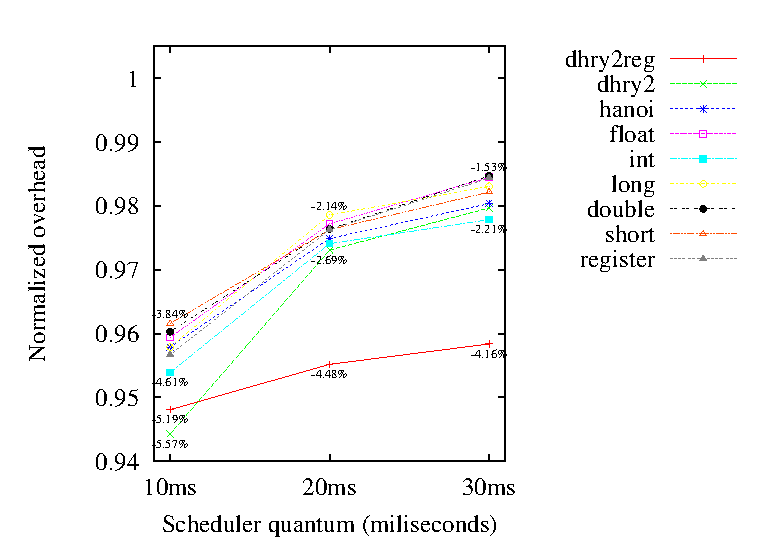
\includegraphics[width=0.6\textwidth]{chapter6/figures/bench_cpu}
	\caption{Performance overhead for user-land applications relative to non-virtualized performance.}
	\label{fig:bench_cpu}
\end{figure}

Each benchmark was performed 10,000 times to determine the average execution time. Figures \ref{fig:bench_cpu} and \ref{fig:bench_syscall} shows the normalized performance results for the user-land and syscall application groups. As expected, the overhead increased slightly with a smaller quantum due the increasing hypervisor intervention. In the user-land group, dhry2 was the most affected application with a performance penalty of 5.57\% when compared to a 10ms scheduler quantum. Additionally, most of the applications suffered an overhead of less than 3\% with a 30ms scheduler quantum. The syscall group suffered a greater performance impact since the benchmark force context-switching between the user and kernel-space in the Linux guest. In the worst case, the syscall close resulted in a penalty of 15.25\% performance loss with a 10ms scheduler quantum. However, for the majority of the cases the overhead was lower than 9\%. 

\begin{figure}[!hbtp]
	\centering
	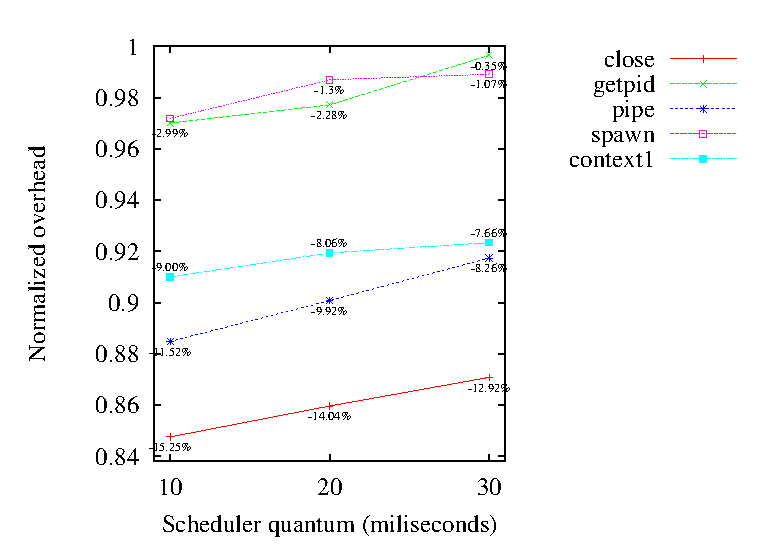
\includegraphics[width=0.6\textwidth]{chapter6/figures/bench_syscall}
	\caption{Performance overhead for syscall applications relative to non-virtualized performance.}
	\label{fig:bench_syscall}
\end{figure}


\subsection{IO-bound Benchmark}  

The Hellfire Hypervisor supports the SEAD-3's network device directly mapped to the Linux guest allowing it to receive network packages without any hypervisor intervention. The Iperf tool was used to measure the network bandwidth between the SEAD-3 board and a Linux host. Thus, it was possible to determine how our virtualization layer affects the I/O performance of the network device when directly mapped. Iperf consists of a client/server application originally developed by NLANR/DAST as a tool for measuring maximum TCP and UDP bandwidth performance \cite{iperf2004}. In this experiment, the Iperf server was executed on a Linux host and the Iperf client on the SEAD-3 board. Thus, the Iperf TCP bandwidth was measured for 1 minute for each experiment case. Figure \ref{fig:iperf} shows the results. The throughput was 8.32 Mbits/second for the native Linux execution. With a 30 ms scheduler quantum, the overhead was 1.84\%. As expected, the overhead increased slightly with a smaller quantum reaching 4.39\% for a 10 ms quantum. Even with smaller quanta, the overall results are optimistic and can be attributed to minimal hypervisor intervention. 

\begin{figure}[!hbtp]
	\centering
	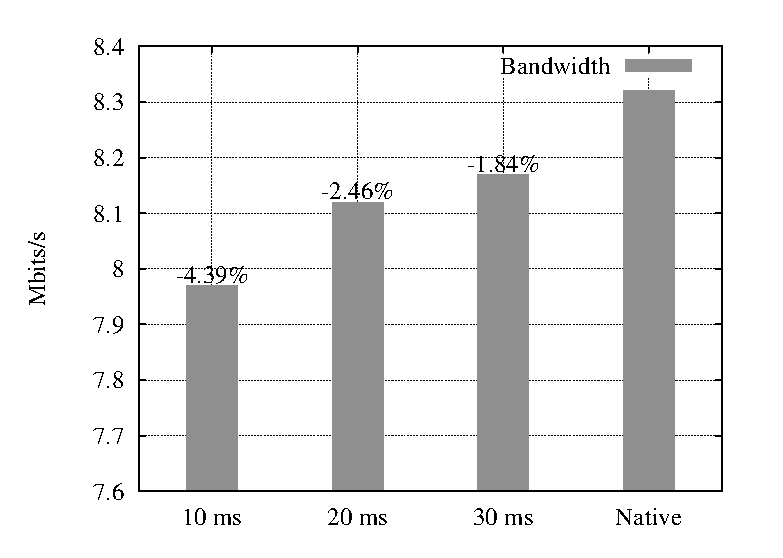
\includegraphics[width=0.6\textwidth]{chapter6/figures/iperf}
	\caption{Iperf bandwidth results for TCP protocol comparing native versus virtualized execution with different hypervisor's scheduler quantum.}
	\label{fig:iperf}
\end{figure}
    
\section{Overhead Impact on HellfireOS} 
\label{section:hellfireOverhead}

This section evaluates the virtualization overhead imposed to the Hellfire OS. The HellfireOS's kernel executes only in kernel mode. Thus, it does not perform memory isolation between tasks because it does not implement memory management. However, the HellfireOS can execute on small processors without MMU support. Two different benchmarks were ported to the RTOS for evaluation purposes. The first algorithm was the adaptive differential pulse-code modulation (ADPCM)  \cite{cummiskey1973}. ADPCM is a technique to convert analog sound to binary information. It is used for voice communication and sound storage. The second was a data compression algorithm, where only compression is done in a buffer containing totally random data. The implementation of this algorithms was obtained from the WCET Project\footnote{http://www.mrtc.mdh.se/projects/wcet/benchmarks.html}, which keeps a large number of benchmark programs. Thus, the source-code was ported to the HellfireOS' APIs.

\begin{figure}[!hbtp]
	\centering
	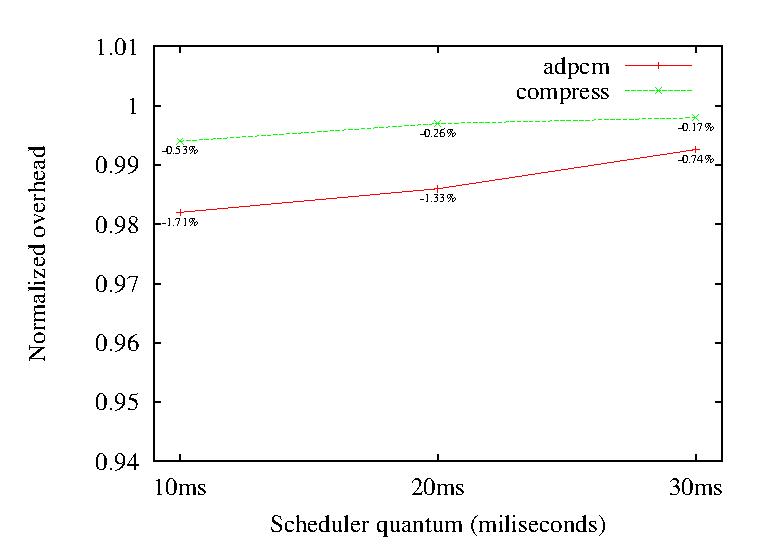
\includegraphics[width=0.6\textwidth]{chapter6/figures/bench_cpu_hell}
	\caption{Performance overhead for CPU intensive applications relative to non-virtualized performance.}
	\label{fig:bench_cpu_hell}
\end{figure}

Both algorithms were performed natively and virtualized with hypervisor scheduler's quantum of 10, 20 and 30ms. The average time for 10,000 executions for each algorithm was obtained. Figure \ref{fig:bench_cpu_hell} shows the normalized results relative to non-virtualized execution. The worst case overhead was 1.71\% for the ADPCM algorithm executing with a scheduler quantum of 10ms. The measured overhead is still smaller than the overhead for Linux CPU-Bound applications (see Figure \ref{fig:bench_cpu}). Despite the HellfireOS to be a lightweight RTOS requiring fewer computation resources, the set of processor resources saved during context-switching is the same of the Linux. A possible explanation for the lower overhead in the HellfireOS is cache effects since the code size impact over the processor's cache was not considered in this study. Linux has a larger code size than HellfireOS what can make it more susceptible to cache effects when submitted to hypervisor interventions. However, more research is necessary to determine the exact cause of the smaller overhead in the HellfireOS benchmarks. 



\section{Interrupt Delivery Delay}
\label{section6:interruption-delay}

This experiment was performed to test the effectiveness of the fast interrupt delivery mechanism as described in Section \ref{section5:interrupt}. Thus, the following experiments show how the response delay of the OS's interrupt handler is affected by the hypervisor interference and how the proposed solution can improve overall system responsiveness. The virtualized system setup consisted of a Linux guest with a variable number of concurrent VMs executing HellfireOS instances. The Ethernet device was directly mapped to the Linux guest. For interrupt delay measurement, the Internet Control Message Protocol (ICMP) was used to send echo request messages from an Intel Xeon server running Debian Linux 7.8 directly connected to the SEAD-3 board. For all test cases, ICMP messages were sent at intervals of 50 milliseconds (20Hz) using the Linux ping application\footnote{http://linux.die.net/man/8/ping}. Each test case consisted of 10,000 echo request messages followed by their respective response messages (echo reply). Thus, the round-trip time (RTT) \cite{tanenbaum2011} of the messages for network communication with the SEAD-3 board was determined. Delays in the Linux interrupt handler caused by the hypervisor impacting directly in the RTT were expected. Finally, the average delay ($\overline{x}$), standard deviation ($s$), median ($m$) and the $95^{th}$ percentile ($p^{th}$) for the RTT of the messages were determined. Results for the Linux/MIPS native (non-virtualized) execution can be viewed in Table \ref{table:delaylinux}. Table \ref{table:delay} shows the results of all experiments performed using virtualization. Lines three and five depict the behavior of the recycled quantum and reset quantum policies with half of the VMs marked as non-preemptable. Figure \ref{fig:native} shows the corresponding histogram for the RTT of native Linux execution messages. The data sets used to generate the results of the lines 1 to 5 of the Table \ref{table:delay} are represented in the histograms of the Figures \ref{fig:non-policy}, \ref{fig:fast-recycling}, \ref{fig:fast-reset}, \ref{fig:fast-recycling-preempt} and \ref{fig:fast-reset-preempt}.

%Figures \ref{fig:histogram_2vm}, \ref{fig:histogram_4vm} and \ref{fig:histogram_6vm} depict the histogram for the RTT of the messages  for 2, 4 and 6 VMs.

\begin{sidewaystable}[!hbtp]
\centering
\caption{Average ($\overline{x}$), standard deviation ($s$), median ($m$) and $95^{th}$ percentile ($p^{th}$) for RTT of the messages in milliseconds for Linux native execution.}
\label{table:delaylinux}
\begin{tabular}{lllll}
\hline \hline
\multicolumn{1}{c}{\textbf{Strategy}} & \multicolumn{1}{c}{\textbf{$\overline{x}$}} & \multicolumn{1}{c}{\textbf{$s$}} & \multicolumn{1}{c}{\textbf{$m$}} & \multicolumn{1}{c}{\textbf{$p^{th}$}} \\ \hline
\textbf{Linux interrupt police}       & 1.073                          & 0.107                          & 1.05                           & 1.24                           \\ \hline
\end{tabular}
\vspace{2\baselineskip}
\caption{Average ($\overline{x}$), standard deviation ($s$), median ($m$) and $95^{th}$ percentile ($p^{th}$) for RTT of the messages in milliseconds for virtualized Linux execution.}
\label{table:delay}
\begin{tabular}{llllllllllllll}
\hline \hline
\multirow{2}{*}{\textbf{\#}} & \multicolumn{1}{c}{\multirow{2}{*}{\textbf{Strategy}}} & \multicolumn{4}{c}{\textbf{2 VMs}}                & \multicolumn{4}{c}{\textbf{4 VMs}}                & \multicolumn{4}{c}{\textbf{6 VMs}}                \\ \cline{3-14} 
                             & \multicolumn{1}{c}{}                                   & \textbf{$\overline{x}$} & \textbf{$s$} & \textbf{$m$} & \textbf{$p^{th}$} & \textbf{$\overline{x}$} & \textbf{$s$} & \textbf{$m$} & \textbf{$p^{th}$} & \textbf{$\overline{x}$} & \textbf{$s$} & \textbf{$m$} & \textbf{$p^{th}$} \\ \hline
\textbf{1}                   & \textbf{Without interrupt police}                      & 9.35       & 10.21      & 2.73       & 29.5       & 30.7       & 29.6       & 86.4       & 66.29      & 66.29      & 49.40      & 66.90      & 145        \\
\textbf{2}                   & \textbf{Recycled quantum (R.Q.)}                      & 1.87       & 4.09       & 1.2        & 1.83       & 12.05      & 1.56       & 5.52       & 6.90       & 6.90       & 21.04      & 1.44       & 50.4       \\
\textbf{3}                   & \textbf{R.Q. with non-preempt. VCPU}                   & 9.28       & 10.16      & 2.70       & 29.1       & 12.90      & 1.66       & 29.1       & 9.72       & 9.72       & 19.83      & 1.68       & 31.5       \\
\textbf{4}                   & \textbf{Reset quantum (Res.Q.)}                        & 1.29       & 0.81       & 1.11       & 1.69       & 2.49       & 1.55       & 1.85       & 2.50       & 2.50       & 10.39      & 1.22       & 1.82       \\
\textbf{5}                   & \textbf{Res.Q. with non-preempt. VCPU}                 & 2.86       & 3.17       & 1.1        & 9.89       & 8.61       & 8.19       & 2.07       & 21.1       & 10.49      & 12.32      & 1.71       & 30.7       \\ \hline
\end{tabular}
\end{sidewaystable}


\begin{figure}[!hbtp]
	\centering
	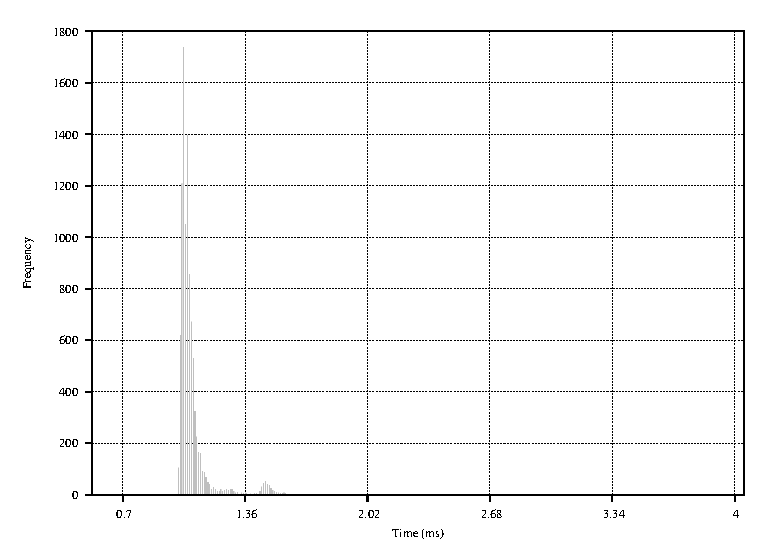
\includegraphics[width=0.45\textwidth]{chapter6/figures/ping_native}
	\caption{Histogram for RTT of the messages for native execution of the Linux/MIPS.}
	\label{fig:native}
\end{figure}

Once the native response time was obtained, the results were compared to virtualized instances of the Linux/MIPS. For each test case, the guest Linux/MIPS shared the processor with VCPUs in different system configurations: 2 VMs (one Linux/MIPS and one BE-VCPU), 4 VMs (one Linux/MIPS and three BE-VCPUs) and 6 VMs (one Linux/MIPS and five BE-VCPUs). Each BE-VCPU was performing the HellfireOS as a guest during the tests. For each configuration, tests were performed without any specific policy, consequently increasing the response delay. Line one of the Table \ref{table:delay} shows that the delay growth is proportional to the increasing number of concurrent VMs. Figures \ref{fig:2vm}, \ref{fig:4vm} and \ref{fig:6vm} show the corresponding histogram to the RTT of the messages to the configuration of 2, 4 and 6 VMs, respectively. Observe the increased horizontal scale of the histogram in the figures. These results show that the hypervisor significantly affected the response time when compared to native results. This was expected since the VMs were scheduled in a round-robin algorithm, and an interrupt on the Ethernet device must wait for the next Linux/MIPS execution. Moreover, the hypervisor scheduler time quantum is 30 milliseconds. For example, in a system configuration of 4 VMs the delay to handle an interrupt can be up to 90 milliseconds if the guest Linux/MIPS is the last in the round-robin queue. 

\begin{figure}[!hbtp]
\centering
\subfigure[Two VMs.]{
    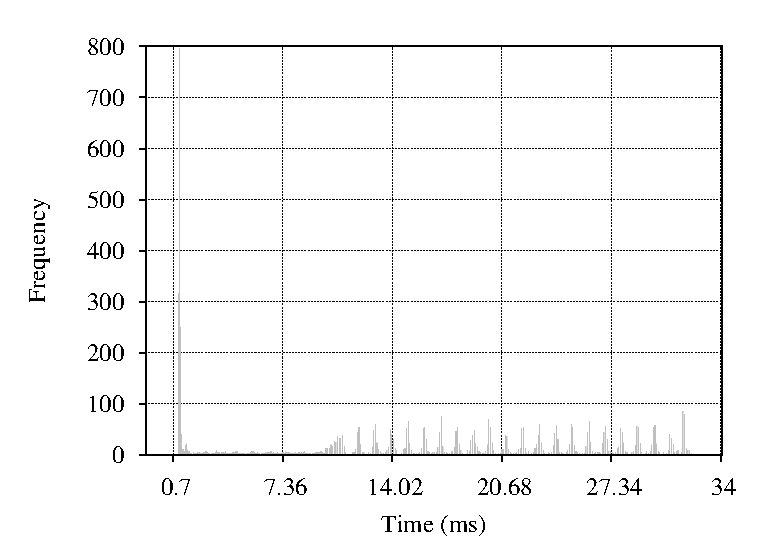
\includegraphics[width=.315\textwidth]{chapter6/figures/2VM}
    \label{fig:2vm}
}
\subfigure[Four VMs.]{
    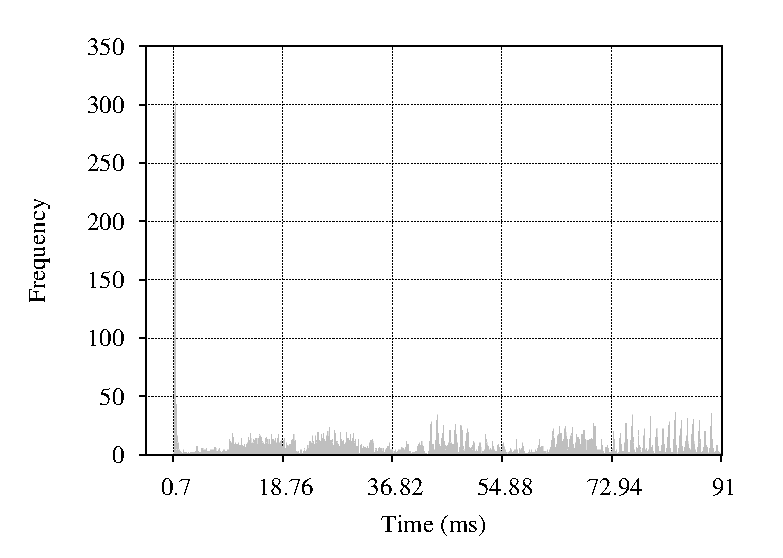
\includegraphics[width=.315\textwidth]{chapter6/figures/4VM}
    \label{fig:4vm}
}
\subfigure[Six VMs.]{
    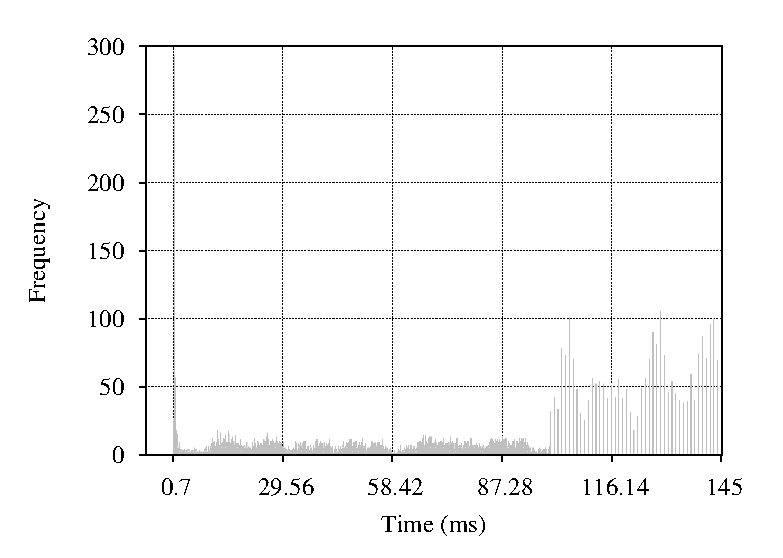
\includegraphics[width=.315\textwidth]{chapter6/figures/6VM}
    \label{fig:6vm}
}
\captionsetup{justification=centering}
\caption{Histogram for RTT of the messages without policy.}
\label{fig:non-policy}
\end{figure}

\begin{figure}[!hbtp]
\centering
\subfigure[Two VMs.]{
    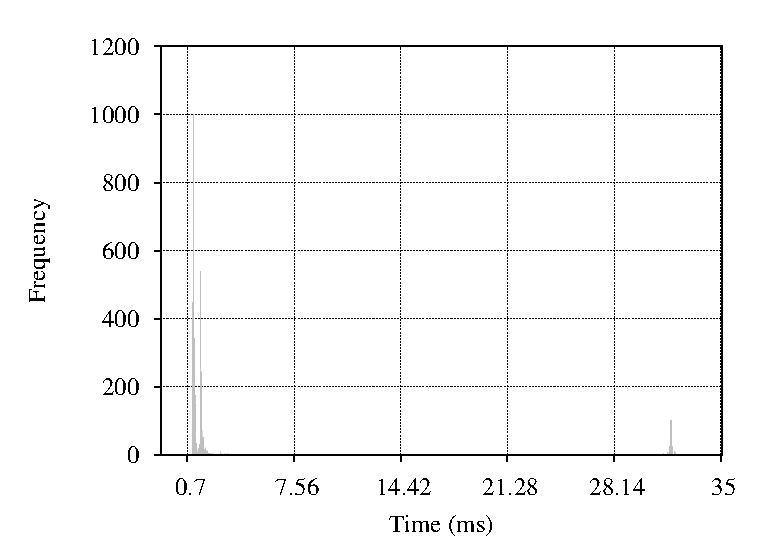
\includegraphics[width=.315\textwidth]{chapter6/figures/2VM-fast-same}
    \label{fig:2vm-fast-same}
}
\subfigure[Four VMs.]{
    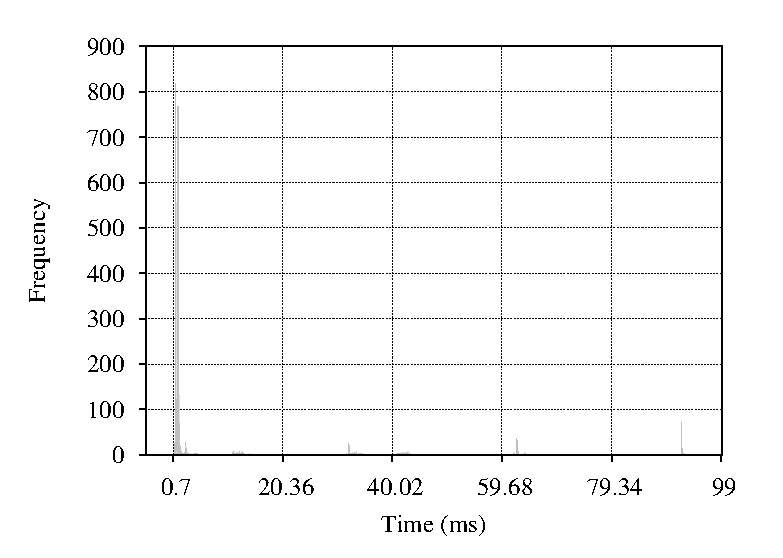
\includegraphics[width=.315\textwidth]{chapter6/figures/4VM-fast-same}
    \label{fig:4vm-fast-same}
}
\subfigure[Six VMs.]{
    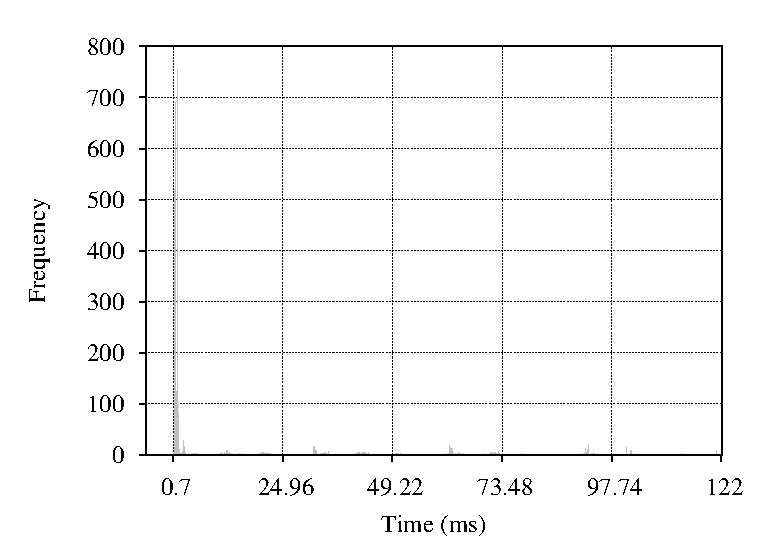
\includegraphics[width=.315\textwidth]{chapter6/figures/6VM-fast-same}
    \label{fig:6vm-fast-same}
}
\captionsetup{justification=centering}
\caption{Histogram for RTT of the messages with fast interrupt policy and quantum recycling.}
\label{fig:fast-recycling}
\end{figure}


%\begin{figure}[!hbtp]
%\centering
%\subfigure[Without policy.]{
%    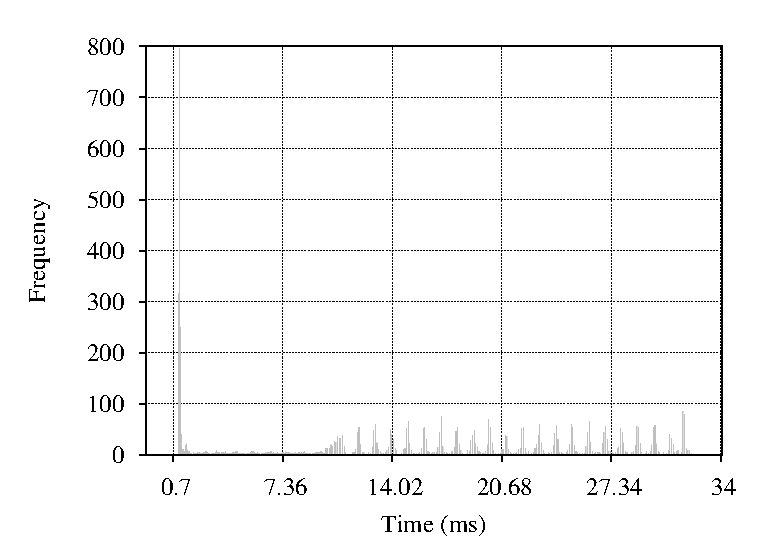
\includegraphics[width=.45\textwidth]{chapter6/figures/2VM}
%    \label{fig:2vm}
%}
%\subfigure[Fast interrupt policy and quantum recycling.]{
%    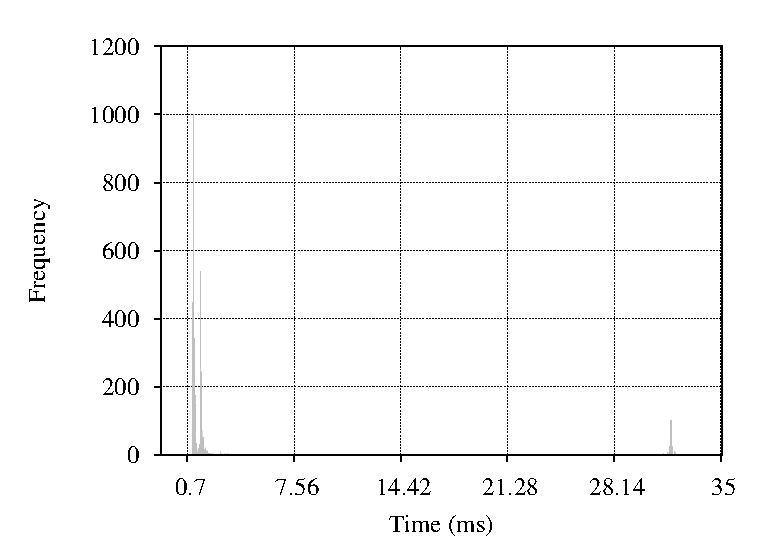
\includegraphics[width=.45\textwidth]{chapter6/figures/2VM-fast-same}
%    \label{fig:2vm-fast-same}
%}

%\subfigure[Fast interrupt policy and quantum reset.]{
%    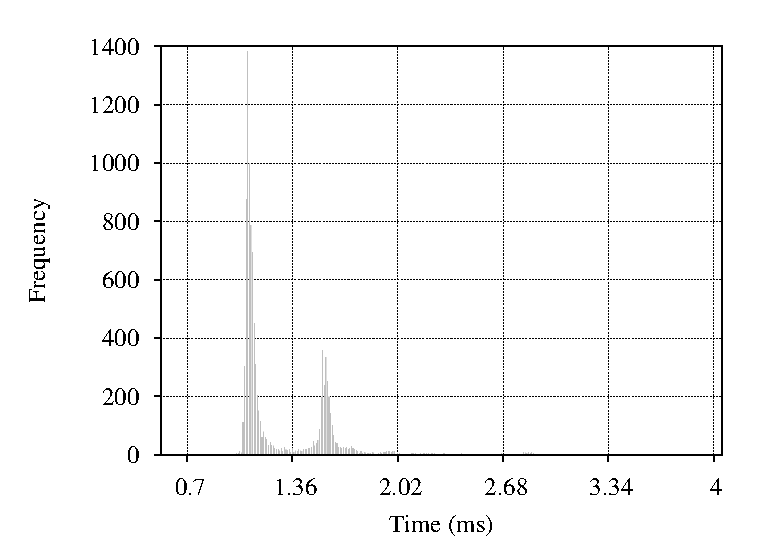
\includegraphics[width=.45\textwidth]{chapter6/figures/2VM-fast-new}
%    \label{fig:2vm-fast-new}
%}
%\subfigure[Fast interrupt policy and quantum reset with two non-preemptable VCPUs.]{
%    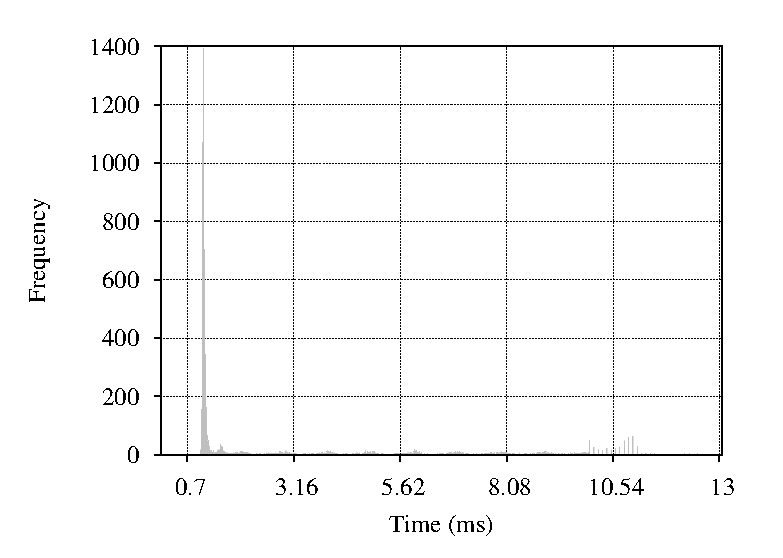
\includegraphics[width=.45\textwidth]{chapter6/figures/2VM-fast-new-1RTOS}
%    \label{fig:2vm-fast-new-rtos}
%}

%\subfigure[Fast interrupt policy and quantum recycling with two non-preemptable VCPUs.]{
%    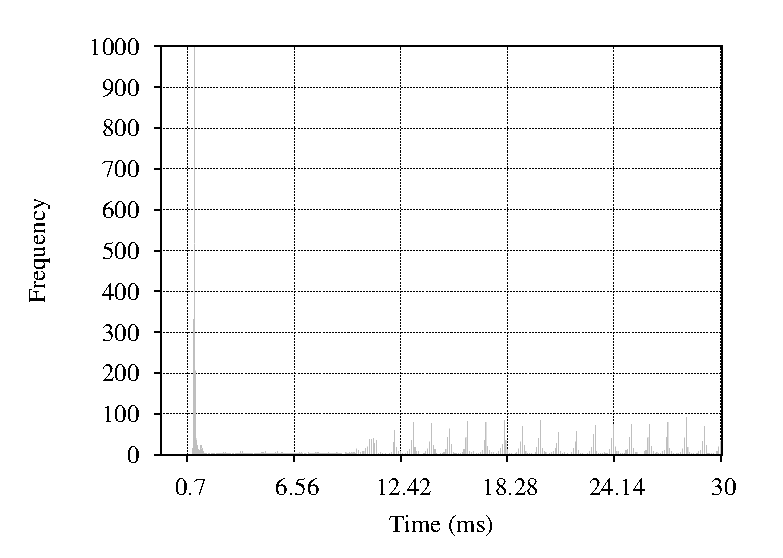
\includegraphics[width=.45\textwidth]{chapter6/figures/2VM-fast-same-1RTOS}
%    \label{fig:2vm-fast-same-rtos}
%}
%\captionsetup{justification=centering}
%\caption{Histogram for messages' RTT for a system configuration of 2 VCPUs.}
%\label{fig:histogram_2vm}
%\end{figure}

%\begin{figure}[!hbtp]
%\centering
%\subfigure[Without policy.]{
%    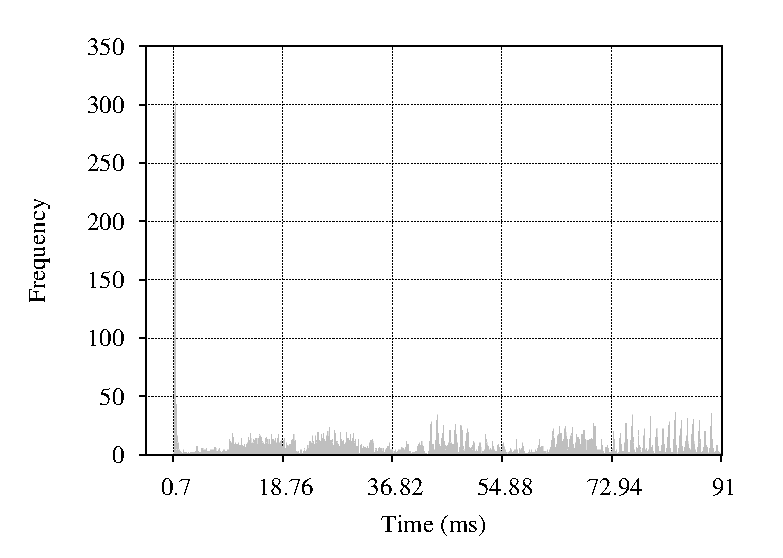
\includegraphics[width=.45\textwidth]{chapter6/figures/4VM}
%    \label{fig:4vm}
%}
%\subfigure[Fast interrupt policy and quantum recycling.]{
%    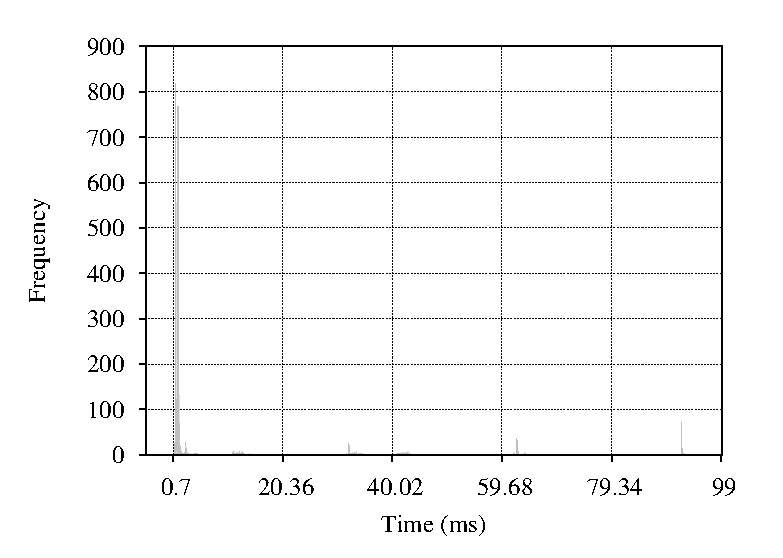
\includegraphics[width=.45\textwidth]{chapter6/figures/4VM-fast-same}
%    \label{fig:4vm-fast-same}
%}

%\subfigure[Fast interrupt policy and quantum reset.]{
%    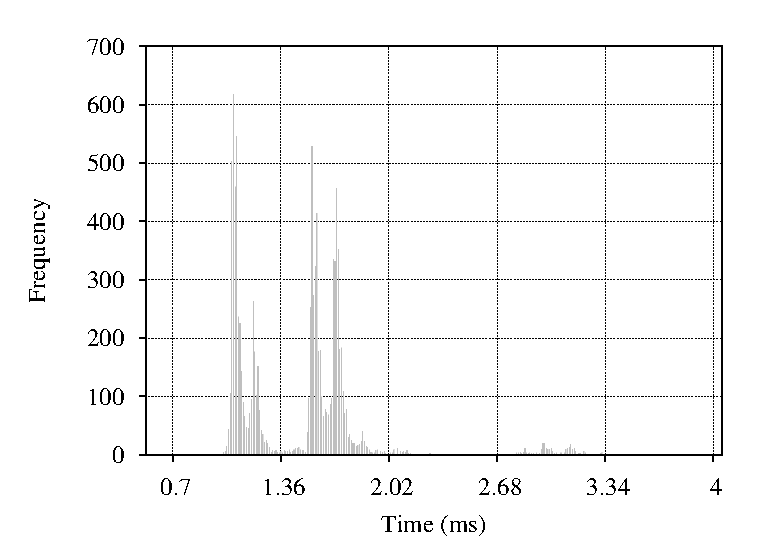
\includegraphics[width=.45\textwidth]{chapter6/figures/4VM-fast-new}
%    \label{fig:4vm-fast-new}
%}
%\subfigure[4 VMs with fast interrupt policy and quantum reset with two non-preemptable VCPUs.]{
%    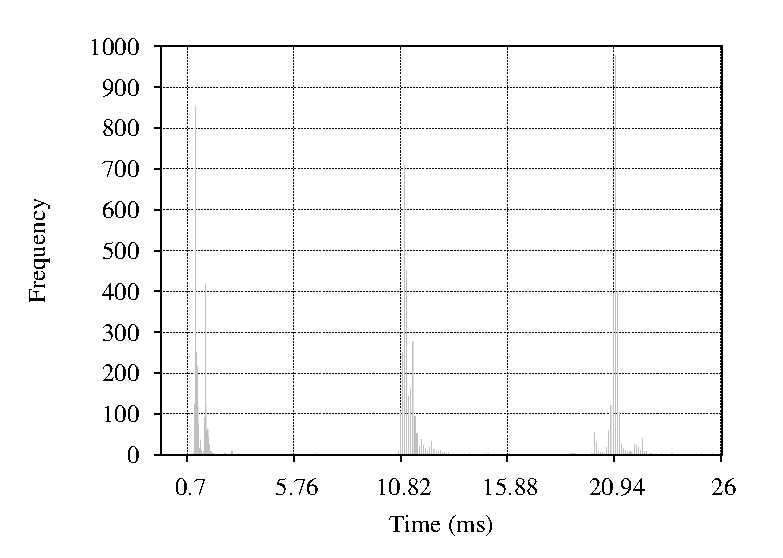
\includegraphics[width=.45\textwidth]{chapter6/figures/4VM-fast-new-2RTOS}
%    \label{fig:4vm-fast-new-rtos}
%}

%\subfigure[4 VMs with fast interrupt policy and quantum recyling with two non-preemptable VCPUs.]{
%    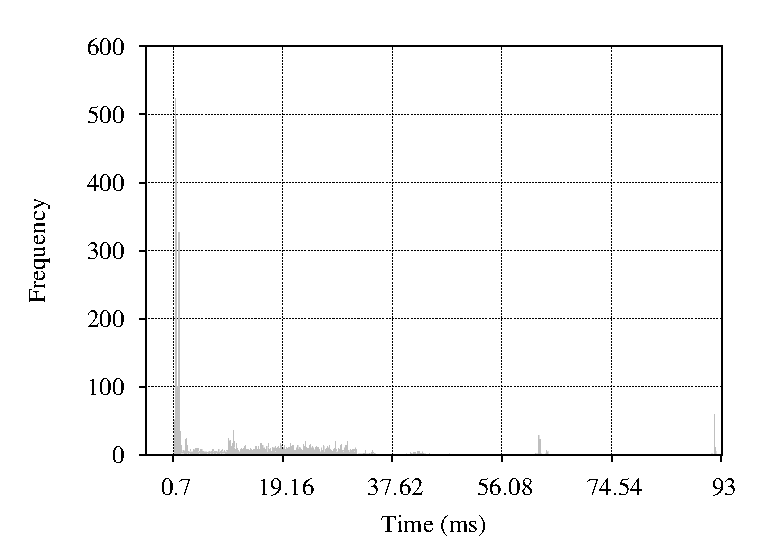
\includegraphics[width=.45\textwidth]{chapter6/figures/4VM-fast-same-2RTOS}
%    \label{fig:4vm-fast-same-rtos}
%}
%\captionsetup{justification=centering}
%\caption{Histogram for messages' RTT for a system configuration of 4 VCPUs.}
%\label{fig:histogram_4vm}
%\end{figure}

After determining how the hypervisor affects the interrupt response time, two different policies were tested to discover which one gives the best approximation to the native response time. Line two of Table \ref{table:delay} (Recycled quantum) shows the results when applied the fast interrupt policy together with the recycled quantum scheme (as explained in Figure \ref{subfig:interruptdelayB}). This technique improves the overall results. However, the recycled quantum mechanism has a drawback. If the remaining of quantum time is not sufficient to finish the interrupt handler routine, it will be finished only in the next guest's execution. Figures \ref{fig:2vm-fast-same}, \ref{fig:4vm-fast-same} and \ref{fig:6vm-fast-same} depict the corresponding histogram of the RTT of the messages for the configuration of 2, 4 and 6 VMs, respectively. Most interrupts have a fast response as shown by the peak near 0.7 milliseconds. For such cases, the interrupt assertion happened during the guest execution or the remaining quantum time was enough for the interrupt handler to finish its job. However, some messages experience a long delay and the response time is close to  multiples of 30 milliseconds. Thus, the remaining quantum time was not enough and the interrupt handler only finished in the next execution. 

\begin{figure}[!hbtp]
\centering
\subfigure[Two VMs.]{
    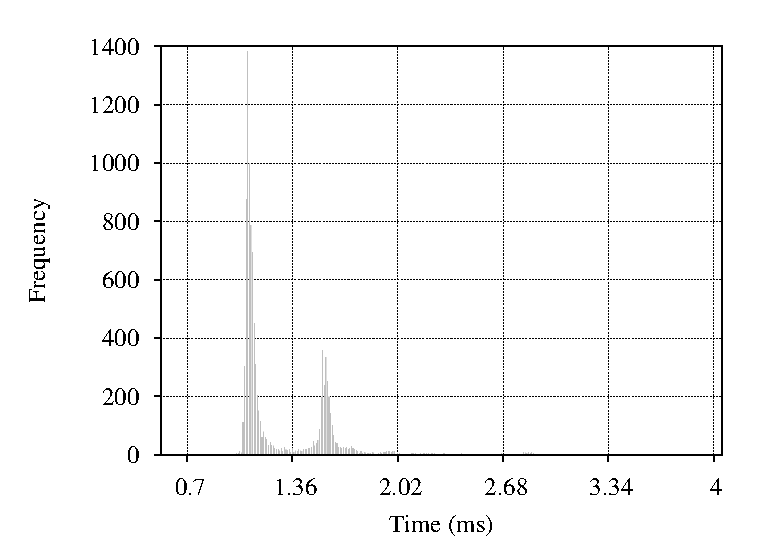
\includegraphics[width=.315\textwidth]{chapter6/figures/2VM-fast-new}
    \label{fig:2vm-fast-new}
}
\subfigure[Four VMs.]{
    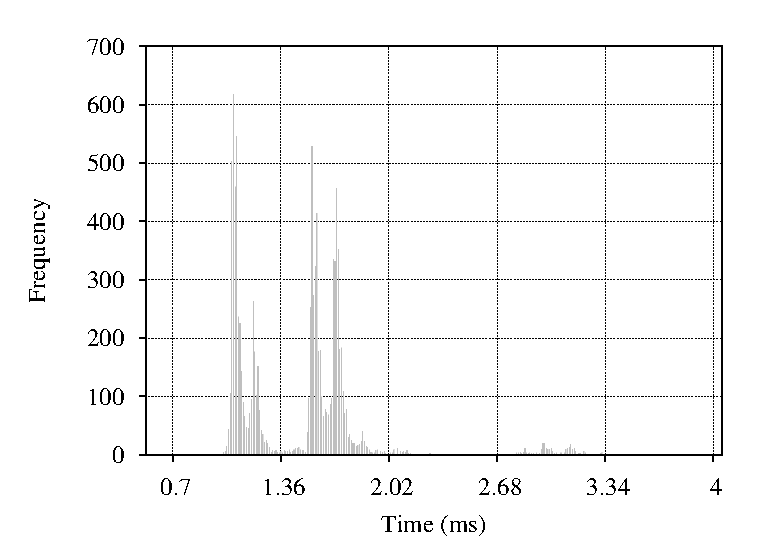
\includegraphics[width=.315\textwidth]{chapter6/figures/4VM-fast-new}
    \label{fig:4vm-fast-new}
}
\subfigure[Six VMs.]{
    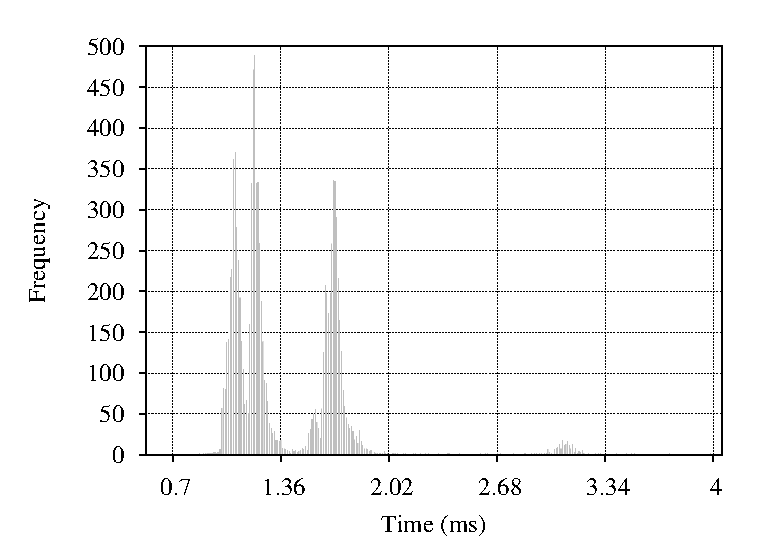
\includegraphics[width=.315\textwidth]{chapter6/figures/6VM-fast-new}
    \label{fig:6vm-fast-new}
}
\captionsetup{justification=centering}
\caption{Histogram for RTT of the messages with fast interrupt policy and quantum reset.}
\label{fig:fast-reset}
\end{figure}


Line four of Table \ref{table:delay} (Reset quantum) shows the results of the fast interrupt policy with a reset quantum scheme. For 2 VM configurations, the average and standard deviation delays are close to native execution. In the 4 and 6 VM system configurations, the results are slightly higher but better than results for the recycled quantum scheme. Figures \ref{fig:2vm-fast-new}, \ref{fig:4vm-fast-new} and \ref{fig:6vm-fast-new} show the corresponding histogram of the RTT of the messages for the configuration of 2, 4 and 6 VMs, respectively. Observe that the horizontal scale in the figure is similar to native execution. These histograms show two peaks. The peak for delays  under one millisecond represents interrupt assertions that happened when the target guest OS was executing. The second peak for delays greater than one millisecond represents interrupt assertions that caused a context switch because the target guest was not executing. 

\begin{figure}[!hbtp]
\centering
\subfigure[Two VMs, one non-preempt.]{
    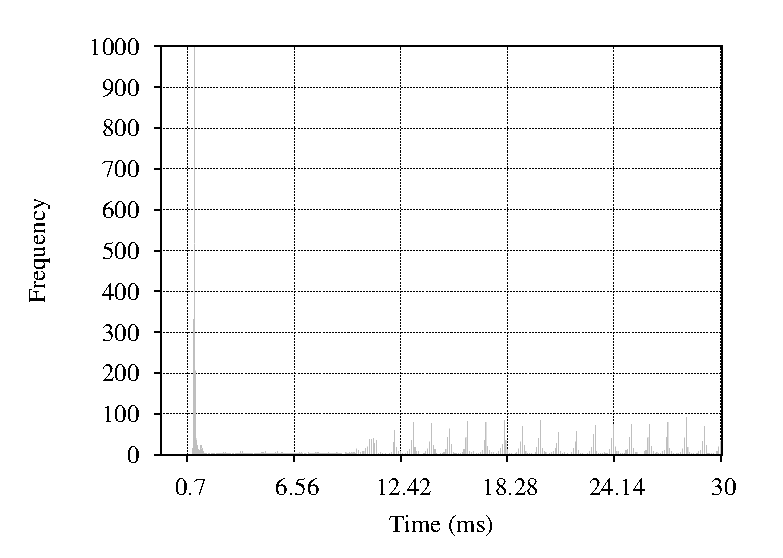
\includegraphics[width=.315\textwidth]{chapter6/figures/2VM-fast-same-1RTOS}
    \label{fig:2vm-fast-same-rtos}
}
\subfigure[Four VMs, two non-preempt.]{
    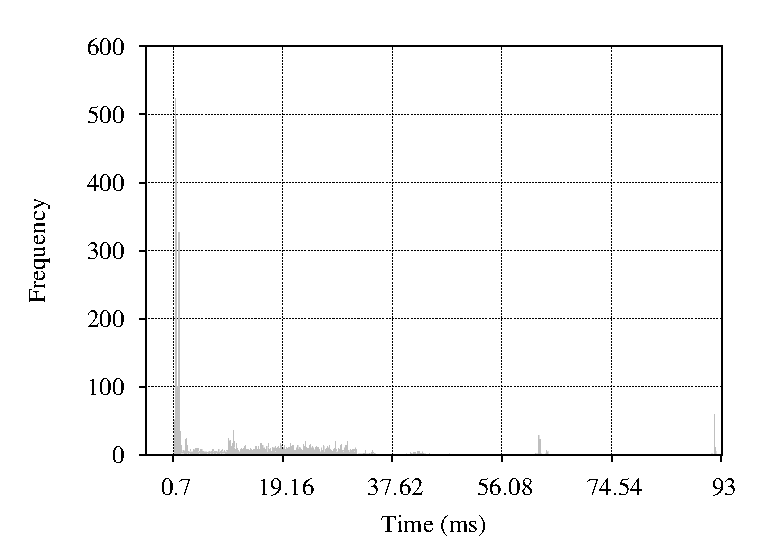
\includegraphics[width=.315\textwidth]{chapter6/figures/4VM-fast-same-2RTOS}
    \label{fig:4vm-fast-same-rtos}
}
\subfigure[Six VMs, three non-preempt.]{
    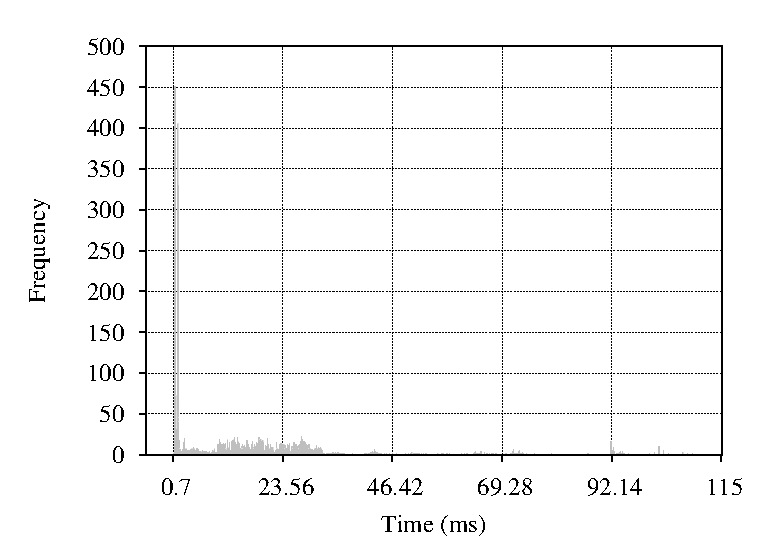
\includegraphics[width=.315\textwidth]{chapter6/figures/6VM-fast-same-3RTOS}
    \label{fig:6vm-fast-same-rtos}
}
\captionsetup{justification=centering}
\caption{Histogram for RTT of the messages with fast interrupt policy and quantum recycling with non-preemptable VCPUs.}
\label{fig:fast-recycling-preempt}
\end{figure}

Finally, lines 3 (R.Q. with non-preempt. RTOS) and 5 (Res.Q. with non-preempt. RTOS) of Table \ref{table:delay} show the results for recycled quantum and reset quantum schemes in the presence of non-preemptive guests. For each configuration, half of the guests were marked as non-preemptive. The presence of non-preemptive guests increased the average and standard deviation delays, but the results are better than the approach without any interrupt policy. Figures \ref{fig:4vm-fast-same-rtos}, \ref{fig:6vm-fast-same-rtos} and \ref{fig:6vm-fast-same-rtos} show the histograms for recycled quantum with non-preemptive guests for 2, 4 and 6 VMs. Figures \ref{fig:4vm-fast-new-rtos}, \ref{fig:6vm-fast-new-rtos} and \ref{fig:6vm-fast-new-rtos} show the histograms for reset quantum with non-preemptive guests for 2, 4 and 6 VMs. 

\begin{figure}[!hbtp]
\centering
\subfigure[Two VMs, one non-preempt.]{
    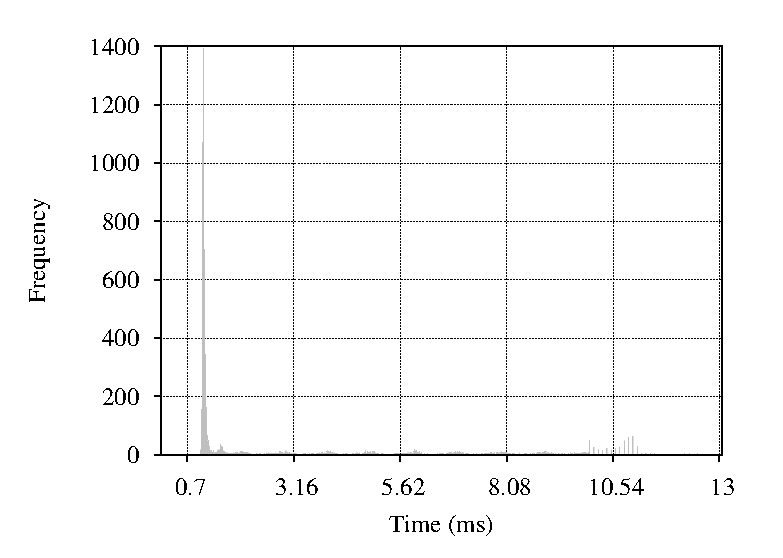
\includegraphics[width=.315\textwidth]{chapter6/figures/2VM-fast-new-1RTOS}
    \label{fig:2vm-fast-new-rtos}
}
\subfigure[Four VMs, two non-preempt.]{
    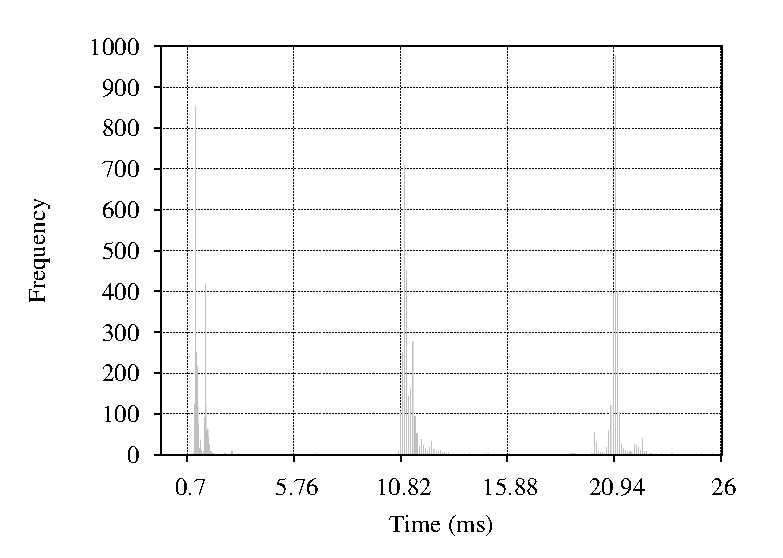
\includegraphics[width=.315\textwidth]{chapter6/figures/4VM-fast-new-2RTOS}
    \label{fig:4vm-fast-new-rtos}
}
\subfigure[Six VMs, three non-preempt.]{
    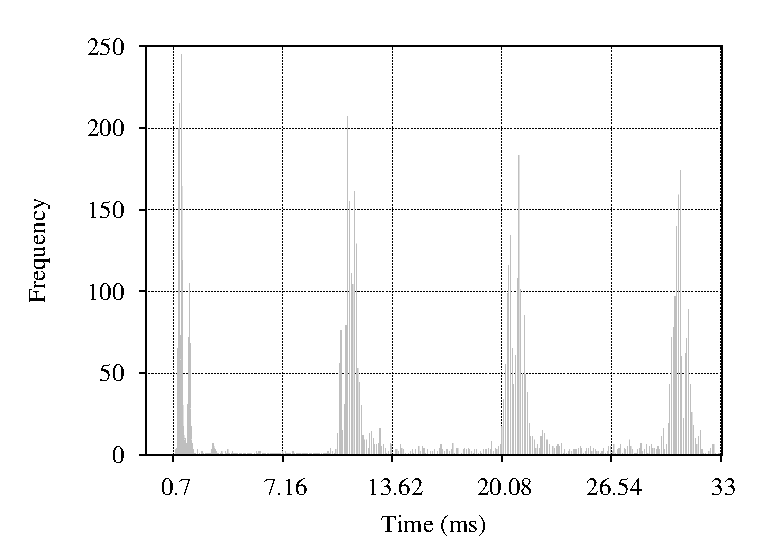
\includegraphics[width=.315\textwidth]{chapter6/figures/6VM-fast-new-3RTOS}
    \label{fig:6vm-fast-new-rtos}
}
\captionsetup{justification=centering}
\caption{Histogram for RTT of the messages with fast interrupt policy and quantum reset with non-preemptable VMs.}
\label{fig:fast-reset-preempt}
\end{figure}

%\begin{figure}[!hbtp]
%\centering
%\subfigure[Without policy.]{
%    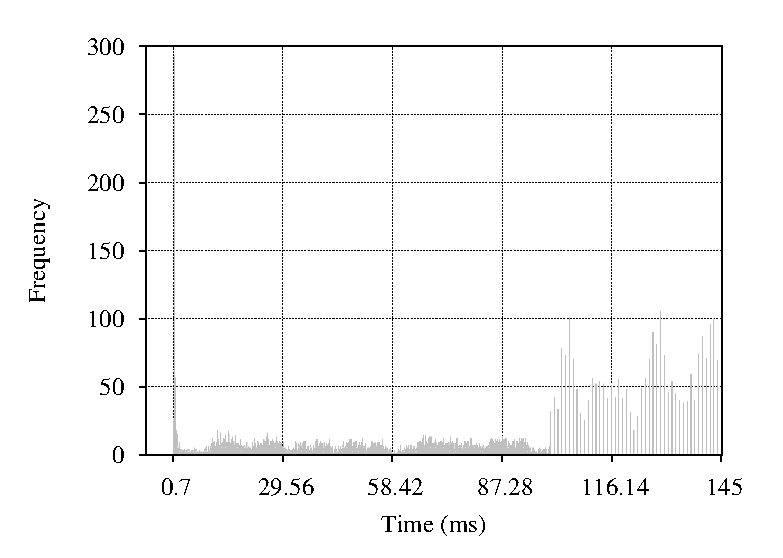
\includegraphics[width=.45\textwidth]{chapter6/figures/6VM}
%    \label{fig:6vm}
%}
%\subfigure[Fast interrupt policy and quantum recycling.]{
%    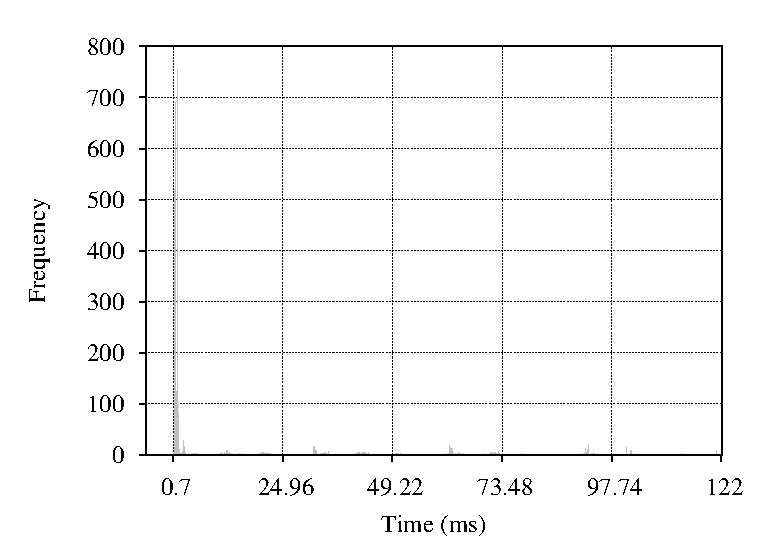
\includegraphics[width=.45\textwidth]{chapter6/figures/6VM-fast-same}
%    \label{fig:6vm-fast-same}
%}

%\subfigure[Fast interrupt policy and quantum reset.]{
%    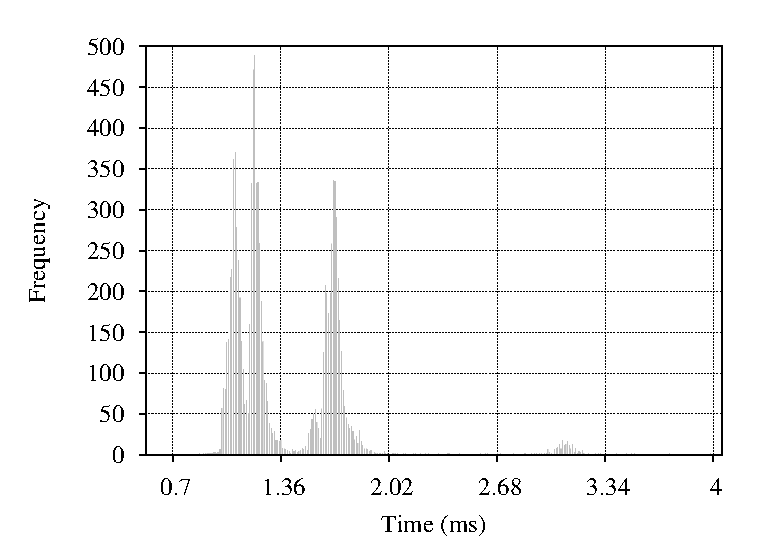
\includegraphics[width=.45\textwidth]{chapter6/figures/6VM-fast-new}
%    \label{fig:6vm-fast-new}
%}
%\subfigure[Fast interrupt policy and quantum reset with three non-preemptable VCPUs.]{
%    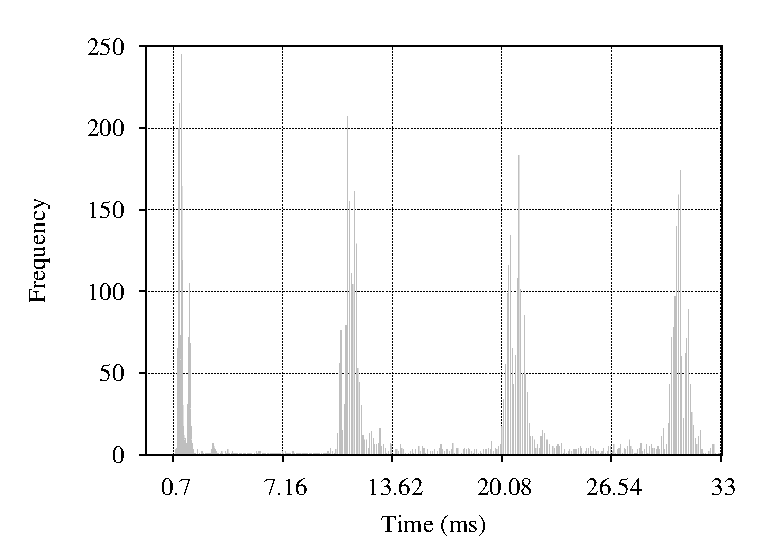
\includegraphics[width=.45\textwidth]{chapter6/figures/6VM-fast-new-3RTOS}
%    \label{fig:6vm-fast-new-rtos}
%}

%\subfigure[Fast interrupt policy and quantum reset with three non-preemptable VCPUs.]{
%    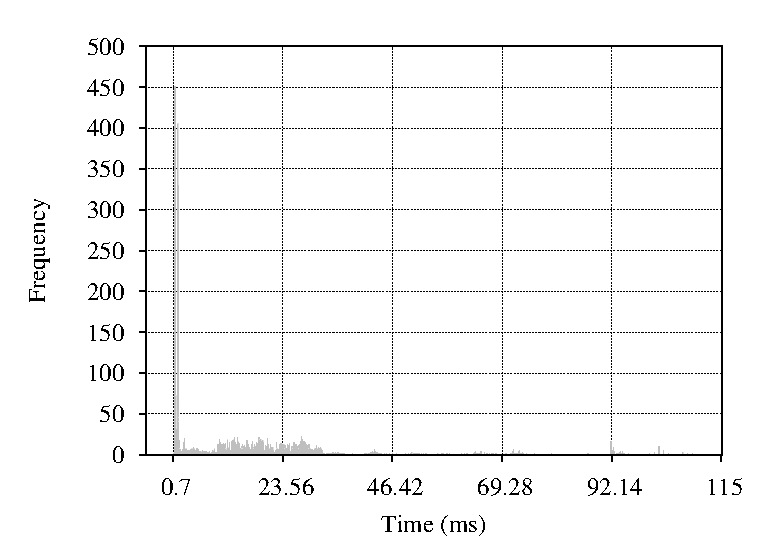
\includegraphics[width=.45\textwidth]{chapter6/figures/6VM-fast-same-3RTOS}
%    \label{fig:6vm-fast-same-rtos}
%}

%\captionsetup{justification=centering}
%\caption{Histogram for messages' RTT for a system configuration of 6 VCPUs.}
%\label{fig:histogram_6vm}
%\end{figure}

The reset quantum scheme associated with the fast interrupt policy presented better results than the recycled quantum. However, this scheme may be disruptive for RTOSs with strict timing constraints and can not be combined with the EDF scheduler algorithm. The EDF implemented computes the next time slot execution of the RT-VCPUs based on the number of quanta performed. The reset quantum scheme breaks the correspondence between time and the completed number of quanta. The recycle quantum mechanism keeps a substantial time isolation between guests. Thus, it must be used when predictability is more important than low response time. Additionally, the fast interrupt policy allows for the reduction of hypervisor interference for  values close to  non-virtualized systems in certain configurations. Finally, the proposed mechanism is flexible and allows for customization of the hypervisor for specific applications for any number of guest OSs. Section \ref{subsection:int_rtvcpus} describes a scenario where the fast interrupt delivery policy is combined with RT-VCPUs.


\section{Inter-VM Communication Response Time}
\label{subsection:intervm}

In order to calculate the RTT of the messages to the inter-VM communication mechanism, it was implemented an echo server application, which replayed all messages received, in the HellfireOS. A client application was implemented in the Linux to send 16, 32 and 64 byte messages after reading the server's response. The measurement of the average RTT for 10,000 messages for each different size resulted in 59.90, 59.90 and 59.99ms with a standard deviation of 0.71ms, 0.71ms and 0.69ms, respectively. An increase in the message size from 16 to 64 bytes did not significantly impact the RTT. The imposed overhead was caused by message copies from the sender's buffer to the target VCPU and to the receiver's buffer. The message exchange mechanism caused an additional copy but allowed  the hypervisor to have better communication control,  similar to pipes in Linux. Figure \ref{fig:intervm} depicts the histogram of the RTT's distribution for 16, 32 and 64 byte messages. In this experiment, we applied our fast interrupt delivery policy. Thus, once the Linux guest sent a message, the hypervisor rescheduled the VMs to the target guest resulting in a faster response and reducing the standard deviation.

\begin{figure}[!hbtp]
	\centering
	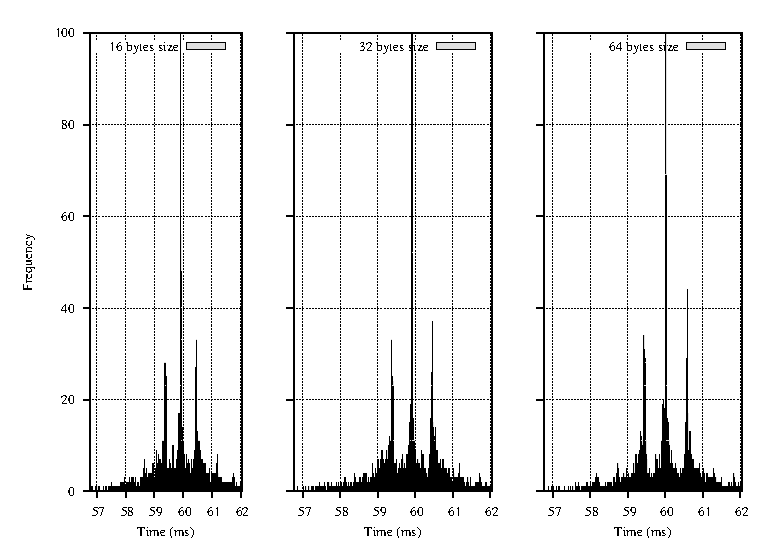
\includegraphics[width=0.50\textwidth]{chapter6/figures/intermv-jitter-3}
	\caption{RTT's histograms for inter-VM communication using the Hellfire Hypervisor communication mechanism.}
	\label{fig:intervm}
\end{figure}


\section{Real-time Services Performance}
\label{section6:realtimeservices}

This section depicts experiments related to real-time services. Thus, RT-VMs are used to provide tasks performed by RT-VCPUs. Subsection \ref{subsection:rtdelay} describes an experiment to determine the real-time scheduler delay caused by the EDF implementation in a system with an increasing number of RT-VCPUs. Subsection \ref{subsection:int_rtvcpus} determines how RT-VCPUs are influenced by external system interrupts. 

\subsection{RT-VCPUs Execution Delay}
\label{subsection:rtdelay}

It is important to determine how long an RT-VCPU takes to start its execution when it is ready. The real-time scheduling involves the timer interrupt handling and the EDF algorithm execution. As mentioned before, the scheduling process adds overhead to the system and the time expended in this process is discounted from the RT-VCPU quantum. To understand how an increasing number of RT-VCPUs affect their execution is important for further improvements in the scheduler algorithm. 

The system configuration for this experiment consisted of a HellfireOS guest responsible for starting and stopping the RT-VCPUs. The RT-VCPUs were managed by a RT-VM. The number of RT-VCPUs in execution in the system were 1, 4 and 8. External interrupts were masked during this experiment. The time needed for RT-VCPU scheduling was determined by reading the counter register when entering  the interrupt handler and calculating the time spent to return to the execution of the VM.

\begin{table}[!hbtp]
\centering
\caption{Average ($\overline{x}$), standard deviation ($s$), median ($m$) and $95^{th}$ percentile ($p^{th}$) for the execution delay on the EDF scheduler in microseconds.}
\label{table:rtdelay}
\begin{tabular}{cllll}
\hline \hline
\textbf{\# RT-VCPUs} & \multicolumn{1}{c}{\textbf{$\overline{x}$}} & \multicolumn{1}{c}{\textbf{$s$}} & \multicolumn{1}{c}{\textbf{$m$}} & \multicolumn{1}{c}{\textbf{$p^{th}$}} \\ \hline
\textbf{1}  & 88.35                          & 4.84                           & 85                             & 94                             \\
\textbf{4}  & 88.66                          & 12.75                          & 91.9                           & 103.2                          \\
\textbf{8}  & 91.44                          & 16.31                          & 97.45                          & 111                            \\ \hline
\end{tabular}
\end{table}


\begin{figure}[!hbtp]
\centering
\subfigure[System with one RT-VCPU.]{
    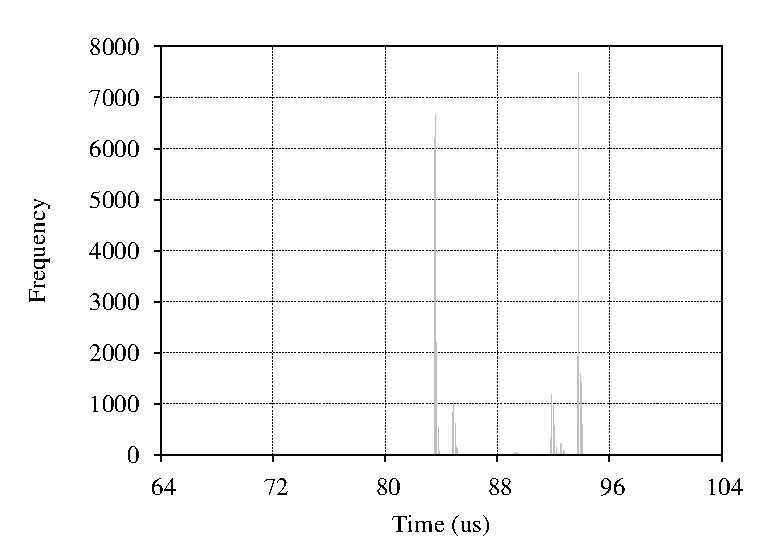
\includegraphics[width=.315\textwidth]{chapter6/figures/rt1}
    \label{fig:rtdelayone}
}
\subfigure[System with four RT-VCPUs.]{
    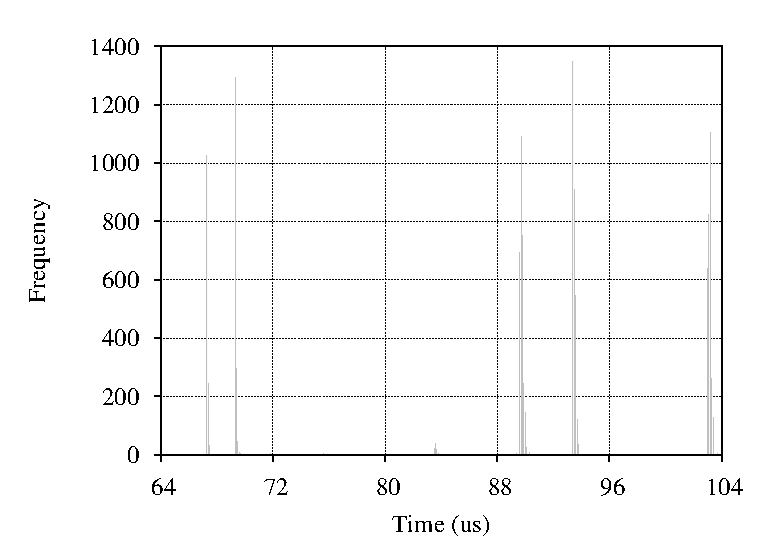
\includegraphics[width=.315\textwidth]{chapter6/figures/rt4}
    \label{fig:rtdelayfour}
}
\subfigure[System with eight RT-VCPUs.]{
    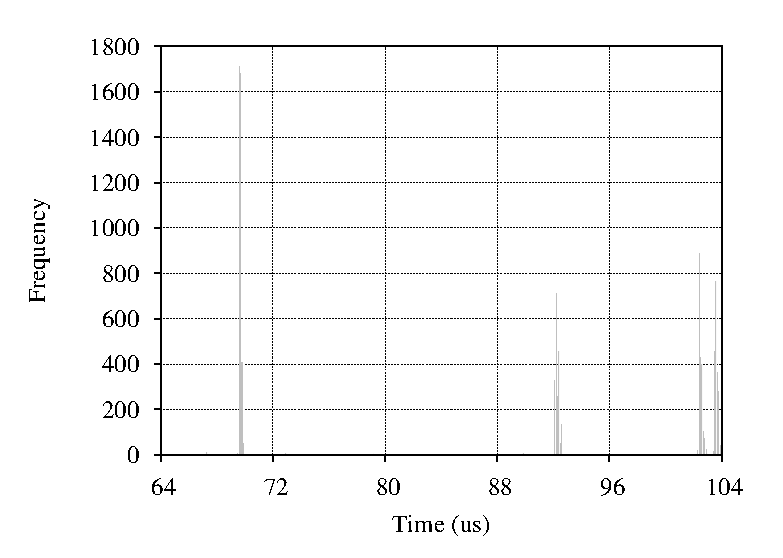
\includegraphics[width=.315\textwidth]{chapter6/figures/rt8}
    \label{fig:rtdelayeigth}
}
\captionsetup{justification=centering}
\caption{Histogram of the execution delay for RT-VCPUs in microseconds.}
\label{fig:rtdelay}
\end{figure}


Table \ref{table:rtdelay} shows the average, standard deviation, median and the $95^{th}$ percentile after 10,000 scheduling rounds for each number for RT-VCPUs in microseconds. The corresponding histograms for the execution of the 1, 4 and 8 RT-VCPUs are shown in Figures \ref{fig:rtdelayone}, \ref{fig:rtdelayfour} and \ref{fig:rtdelayeigth} The average time expended to schedule a RT-VCPU is less than 100 microseconds. When compared to a scheduler quantum of 30ms this represents only 0.003\% of the quantum. However, the standard deviation and the $95^{th}$ percentile increases with a higher number of RT-VCPUs. This is caused by the EDF algorithm implementation that has a complexity of $O(n)$. Despite the increase in the response time to represent only a few microseconds, this can be minimized with a predicable EDF implementation, like proposed by \cite{jagbeer2011}.



\subsection{Interrupt Handling Interference on RT-VCPUs}
\label{subsection:int_rtvcpus}

A sequence of four experiments were performed to show how the Hellfire Hypervisor can be configured to support real-time services while minimizing the interrupt delivery delay on BE-VCPUs. Additionally, these tests determined how RT-VCPUs are influenced by external system interrupts.  For this, the extended real-time services and fast interrupt delivery capabilities were combined in the same virtualized system. The system configuration for this experiment consisted of a Linux guest, a HellfireOS guest and a RT-VM. The Linux guest was responsible for network communication with external devices because it was configured with TCP/IP support and the Ethernet device was directly mapped to it. The HellfireOS was responsible for managing the real-time services (start and stop). The RT-VM implemented a real-time service to perform the ADPCM algorithm (see Subsection \ref{section:hellfireOverhead}). When the algorithm is encoding or decoding for sound reproduction purposes, it must keep a constant bit rate to avoid sound glitches. Thus, the hypervisor must guarantee that concurrent events will not affect the ADPCM execution. 


\begin{figure}[!hbtp]
	\centering
	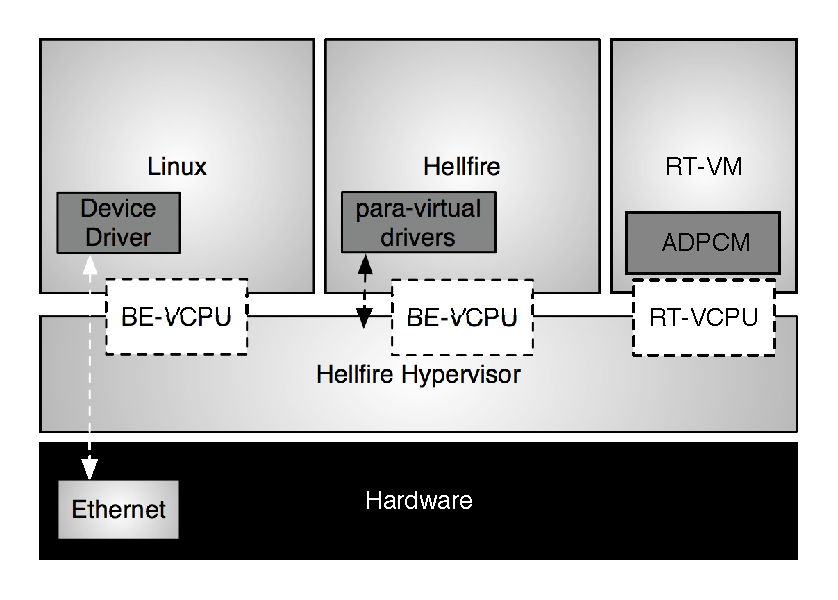
\includegraphics[width=0.40\textwidth]{chapter6/figures/rtsystem}
	\caption{System configuration for the ADPCM execution.}
	\label{fig:rtsystem}
\end{figure}


On the RT-VM, the ADPCM algorithm was mapped to a RT-VCPU that is scheduled by the EDF algorithm, as explained in Subsection \ref{subsection:best-effort-edf}. The real-time parameters of the RT-VCPU were: deadline 10, period 10, and capacity 1. Thus,  a tenth of the processor's time is reserved for the RT-VCPU. The remaining time is available to the BE-VCPUs responsible for executing the Linux and HellfireOS guests. The final system configuration consisted of two BE-VCPUs and 1 RT-VCPU. Figure \ref{fig:rtsystem} shows this arrangement. Similar to the experiment shown in Section \ref{section6:interruption-delay}, the ping tool was used to generate echo request messages from a host computer to the SEAD-3 board at a rate of 20Hz.

\begin{table}[!hbtp]
\centering
\caption{Average ($\overline{x}$), standard deviation ($s$), median ($m$), $95^{th}$ percentile ($p^{th}$), worst execution case (WEC) and best execution case (BEC) to ADPCM encoding and decoding and the RTT of the messages for different system configurations in milliseconds.}
\label{table:rtsystem}
\begin{tabular}{lllllllll}
\hline \hline \\
\textbf{\#}                 & \textbf{System Conf.}                                   & \textbf{Test}     & \textbf{$\overline{x}$} & \textbf{$s$} & \textbf{$m$} & \textbf{$p^{th}$} & \textbf{WEC} & \textbf{BEC} \\ \\ \hline
\multirow{3}{*}{\textbf{1}} & \multirow{3}{*}{\textbf{Execution time}} & \textbf{Encoding} & 1366.58    & 134.21     & 1487       & 1487       & 1487        & 1217        \\
                            &                                                     & \textbf{Decoding} & 1068.94    & 133.1      & 1187       & 1188       & 1188        & 917  \\       
                            &                                                     & \textbf{RTT}      &  1.073 &   0.107 &    1.05 &   1.24     & 3.25   & 0.99                       \\  \hline            
\multirow{3}{*}{\textbf{2}} & \multirow{3}{*}{\textbf{Non policy}}                & \textbf{Encoding} & 1375.27    & 133.16     & 1487       & 1488       & 1488        & 1216        \\
                            &                                                     & \textbf{Decoding} & 1082.17    & 148.63     & 1188       & 1188       & 1189        & 917         \\
                            &                                                     & \textbf{RTT} & 13.37      & 15.1       & 5.78       & 45.5       & 66.6        & 0.78        \\ \hline
\multirow{3}{*}{\textbf{3}} & \multirow{3}{*}{\textbf{Fast policy - non-RT}}        & \textbf{Encoding} & 2004.25    & 546.48     & 2082       & 2705       & 2997        & 1217        \\
                            &                                                     & \textbf{Decoding} & 1505.45    & 497.15     & 1211       & 2390.1     & 2677        & 917         \\
                            &                                                     & \textbf{RTT} & 2.077      & 4.8        & 1.45       & 1.74       & 63.6        & 1.07        \\ \hline
\multirow{3}{*}{\textbf{4}} & \multirow{3}{*}{\textbf{Fast Policy - RT}}            & \textbf{Encoding} & 1378.48    & 132.55     & 1487       & 1488       & 1490        & 1217        \\
                            &                                                     & \textbf{Decoding} & 1081.0     & 132.12     & 1188       & 1188       & 1188        & 917         \\
                            &                                                     & \textbf{RTT} & 3.60       & 7.26       & 1.48       & 20.81      & 65.8        & 1.05        \\ \hline
\end{tabular}
\end{table}

\begin{figure}[!hbtp]
	\centering
	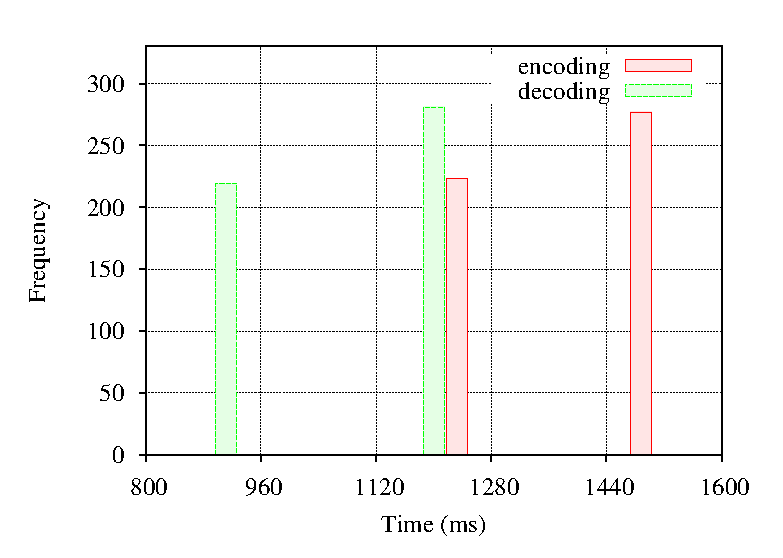
\includegraphics[width=0.50\textwidth]{chapter6/figures/non_int}
	\caption{Histogram of encoding and decoding execution time for the ADPCM algorithm without external interferences.}
	\label{fig:nonint}
\end{figure}


\textbf{Experiment 1.} The first experiment determined how much time the ADPCM algorithm takes to encode and decode a data array. The algorithm was performed during 1,000 encoding and decoding cycles and the time of each execution was recorded. Table \ref{table:rtsystem} shows the numeric results for this experiment in line 1. Additionally, it was plotted in the histogram shown in Figure \ref{fig:nonint}. During this experiment, the RT-VCPU was performed alone and all external interrupts were masked. Thus, obtaining the execution time without the influence of other VCPUs or interrupts. The worst case execution time for encoding was 1,487 ms and 1,217 ms for decoding. Moreover, line one of Table \ref{table:rtsystem} shows the RTT of the messages for native Linux execution for comparison purposes with the upcoming experiments. 

\textbf{Experiment 2.} The second experiment showed the behavior of the ADPCM execution time and the RTT of the messages when the fast delivery policy was not used. This is the simplest configuration, where all interrupts are postponed to the next execution of the target VCPU. This scheme guarantees a temporal isolation to the RT-VCPU since interrupts to other VMs do not preempt its execution. The histogram for 1,000 encoding and decoding cycles is shown in Figure \ref{fig:hist-non-fast}. Additionally, line 2 of the Table \ref{table:rtsystem} shows the numeric results. It confirms that the ADPCM's execution time was not affected by the external interrupts since it is similar to the histogram in Figure \ref{fig:nonint}. However, this scheme had an undesired effect over the RTT of the messages: the average response time increased substantially. Figure \ref{fig:hist-ping-non-fast} is a histogram for 10,000 messages recorded during the experiment. The histogram for the RTT of the messages for native Linux execution can be seen in Figure \ref{fig:native}.

\begin{figure}[!hbtp]
\centering
\subfigure[Histogram of encoding and decoding time for the ADPCM algorithm.]{
    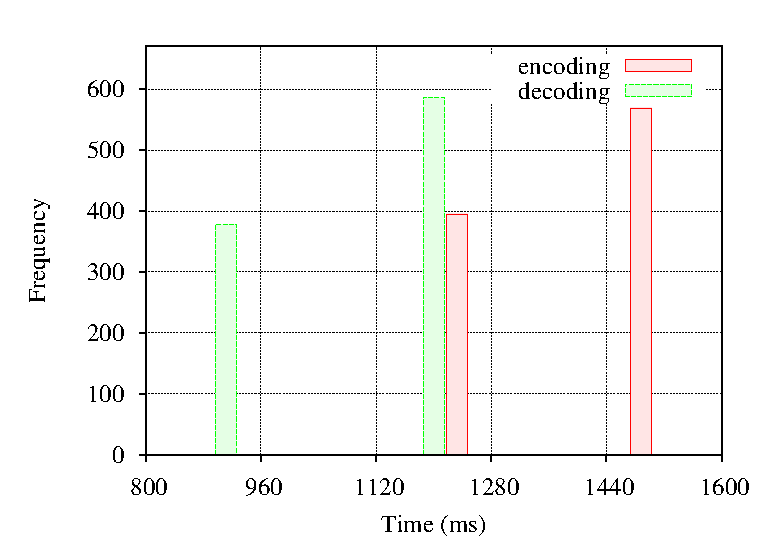
\includegraphics[width=.48\textwidth]{chapter6/figures/20hz_int}
    \label{fig:hist-non-fast}
}
\subfigure[Histogram for RTT of the messages.]{
    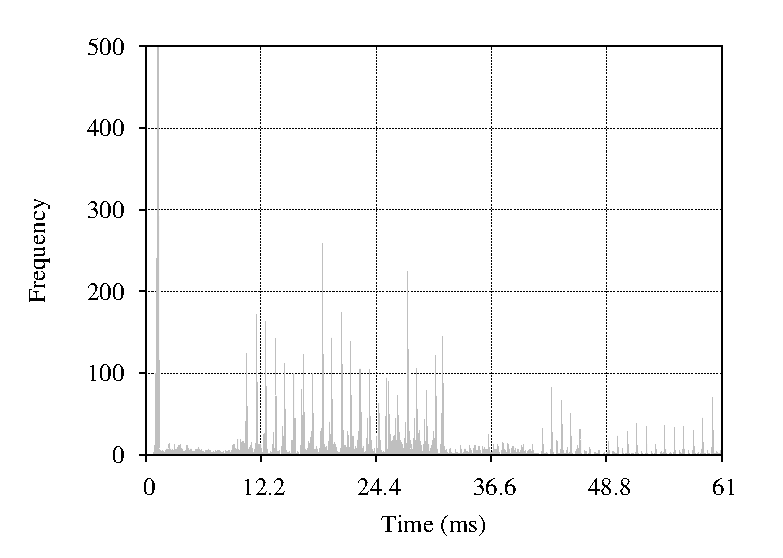
\includegraphics[width=.48\textwidth]{chapter6/figures/ping-non-fast-int}
    \label{fig:hist-ping-non-fast}
}

\captionsetup{justification=centering}
\caption{System response time without the fast interrupt deliver policy and a preemptable RT-VM.}
\label{fig:histogram_nonpremp_nonfast}
\end{figure}

\textbf{Experiment 3.} The third experiment tried to minimize the RTT of the ICMP messages applying the fast interrupt delivery policy. However, the RT-VM was kept as preemptable for an evaluation of how system interrupts can intervene on the RT-VCPU's execution. Thus, both the RT-VCPU and the HellfireOS could be preempted for interrupts targeting the Linux guest. Similar to the previous experiments, 1,000 ADPCM encoding and decoding cycles and 10,000 messages RTT were recorded. Figure \ref{fig:histogram_premp_fast} shows the resulting histograms. The numerical results can be seen in line 3 of Table \ref{table:rtsystem}.

\begin{figure}[!hbtp]
\centering
\subfigure[Histogram of encoding and decoding time for the ADPCM algorithm.]{
    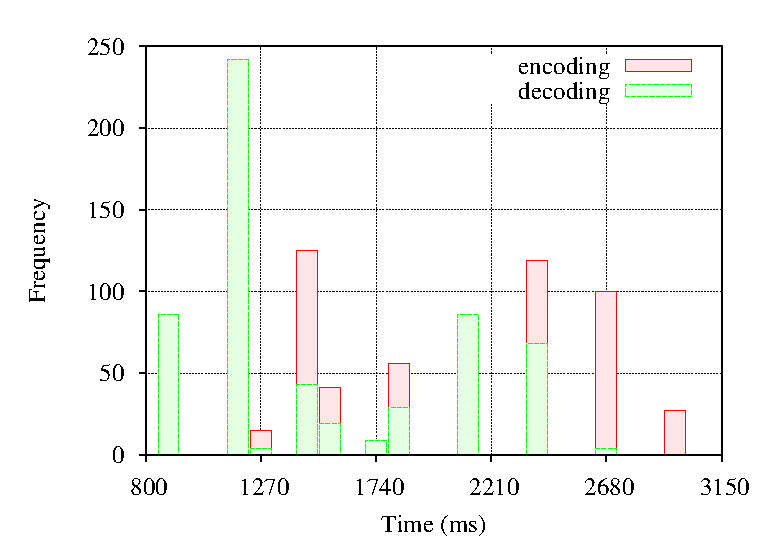
\includegraphics[width=.48\textwidth]{chapter6/figures/nonrt-fast}
    \label{fig:hist-nonrt-fast}
}
\subfigure[Histogram for RTT of the messages.]{
    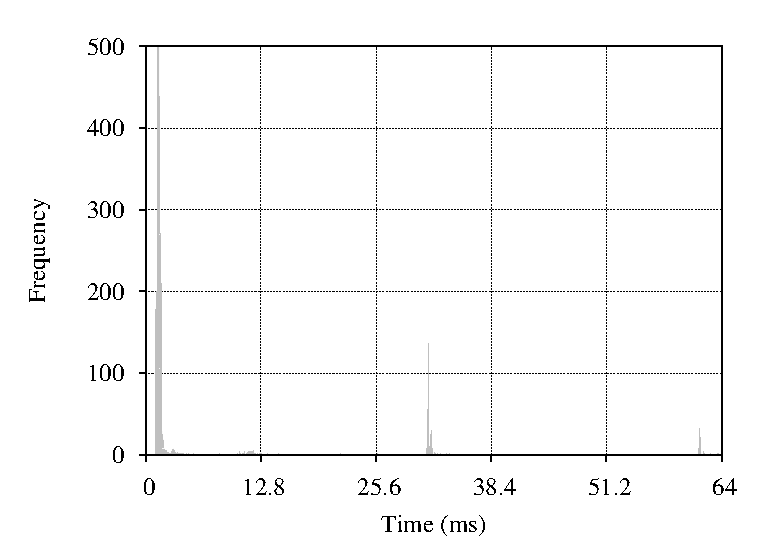
\includegraphics[width=.48\textwidth]{chapter6/figures/ping-nonrt-fast}
    \label{fig:hist-ping-nonrt-fast}
}

\captionsetup{justification=centering}
\caption{System response time with the fast interrupt deliver policy and a preemptable RT-VM.}
\label{fig:histogram_premp_fast}
\end{figure}

Figure \ref{fig:hist-ping-nonrt-fast} and the numerical results show that the RTT of the messages improved significantly. Most of the RTTs were near native execution (see Figure \ref{fig:native}). However, some RTTs suffered a long delay, around 31 ms and 61 ms. This is result of the fast interrupt policy with recycled quantum. The recycled quantum was used to preserve the scheduling time coherency to the EDF algorithm. Despite the reset quantum scheme resulting in an improved interrupt response time, as shown in Section \ref{section6:interruption-delay}, it can not be used in combination with RT-VCPUs. Thus, the long delay is due to the insufficient time remaining in the current quantum. Moreover, the interrupt handling finishes only on the next Linux guest execution. On the other hand, Figure \ref{fig:hist-nonrt-fast} showed that ADPCM execution time was affected, increasing significantly. The numerical results can be seen in line 3 of the Table  \ref{table:rtsystem}.

\textbf{Experiment 4.} The fourth experiment consisted of combining the fast interrupt delivery policy with a non-preemptable RT-VM. This system configuration provides the best temporal isolation for RT-VCPUs while improving the response for external interrupts. This is possible because the fast interrupt delivery policy preempts the VCPUs for faster response time. However, the RT-VM is marked as non-preemptable resulting that its RT-VCPUs cannot be preempted. This guarantees a tenth of the CPU to the  RT-VCPU executing the ADPCM algorithm. 

\begin{figure}[!hbtp]
\centering
\subfigure[Histogram of encoding and decoding time for the ADPCM.]{
    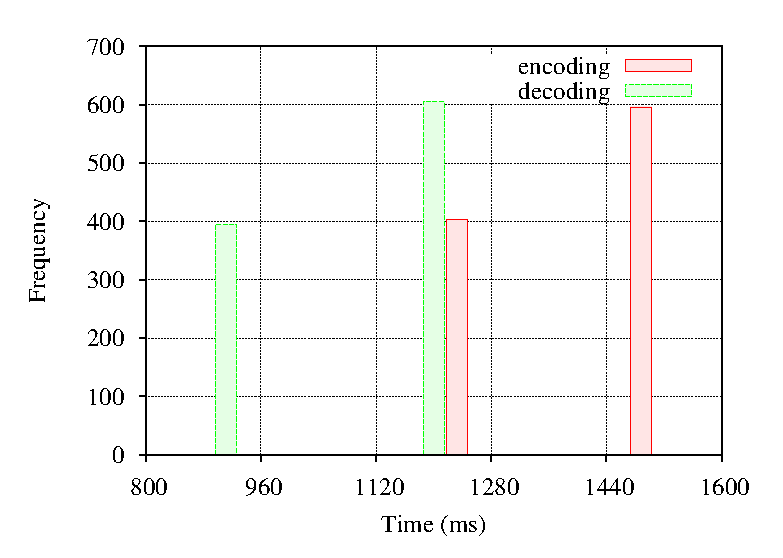
\includegraphics[width=.48\textwidth]{chapter6/figures/rt-fast}
    \label{fig:hist-rt-fast}
}
\subfigure[Histogram for the  RTT of the messages.]{
    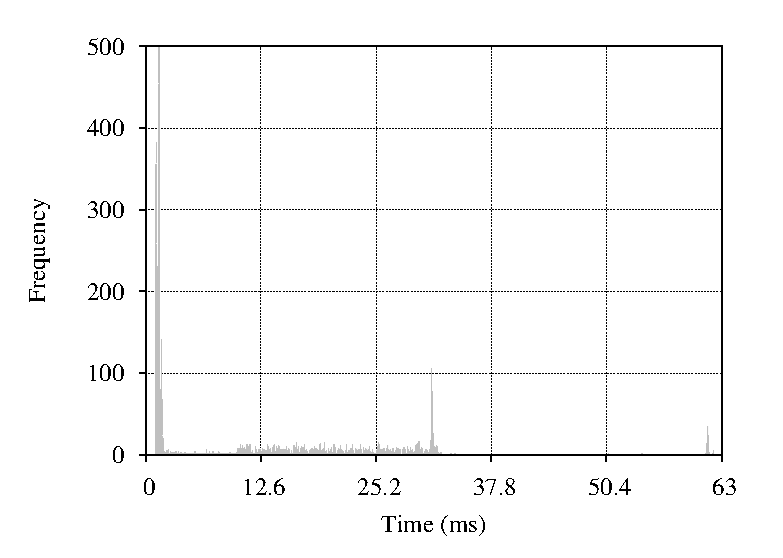
\includegraphics[width=.48\textwidth]{chapter6/figures/ping-rt-fast}
    \label{fig:hist-ping-rt-fast}
}
\captionsetup{justification=centering}
\caption{System response time with the fast interrupt deliver policy and a non-preemptable RT-VM.}
\label{fig:histogram_rt_fast}
\end{figure}

Line 4 of Table \ref{table:rtsystem} shows the numerical results for this experiment. The worst execution case to encoding and decoding the ADPCM algorithm is similar to the execution time presented in line 1 (non external interference). Moreover, the histogram for the execution time shown in Figure \ref{fig:hist-rt-fast} is similar to the histogram in Figure \ref{fig:nonint}. This shows the effectiveness of the temporal isolation provided by the hypervisor. In addition, the RTT of the messages improved significantly. The histogram in Figure \ref{fig:hist-ping-rt-fast} shows that some RTTs are spread between 0.7 and 31ms. This is caused by the RT-VCPU in the RT-VM. The ICMP messages arrived during its execution are delayed until the end of the quantum. The peak near 31ms and 61ms is due to the recycling quantum scheme, as explained before. 


\section{Final Considerations}
\label{section6:finalcons}

This chapter studied the effectiveness of the hypervisor implementation. A sequence of experiments was performed in the SEAD-3 development board to evaluate different aspects of the hypervisor. One important aspect discussed was the footprint. A direct comparison with all other hypervisors studied is not possible because some of them do not mention their footprint. However, the Hellfire Hypervisor's footprint is acceptable for IoT devices, and is similar to the smallest hypervisors with a known  footprint. The overhead impact on Linux was determined using benchmarks for virtualized and non-virtualized executions. User-land applications suffered lower impact than applications that use syscalls intensively. However, the overall overhead is small and comparable to other hypervisors. Moreover, the hypervisors present a low overhead for directly mapped devices. The fast interrupt delivery mechanism was evaluated showing the effectiveness of this policy. This experiment showed that the hardware-assisted virtualization can be used to improve responsiveness while keeping the simplicity of the implementation. The inter-VM communication mechanism presented a considerable overhead caused by the data copies between the VMs and the hypervisor. However, the usage of the hypervisor as a communication arbiter improves the security. Also, shared memory can be used to implement inter-VM communication with lower overhead. Finally, the real-time services were evaluated. The average time expended for RT-VCPU scheduling is lower than 100us in a system with 8 VCPUs. The temporal isolation was tested showing that the fast interrupt policy with non-preemptable RT-VMs is an effective method to combine real-time tasks and fast interrupt handling. The overall results are promising and prove that the hypervisor implementation is efficient in performance and responsiveness. 


\chapter{\label{chapter:conclusions}Conclusions}

This dissertation started by defining the research goal. The objective was to verify hypothesis that is possible to have an embedded lightweight hypervisor capable of supporting the major embedded virtualization requisites. After the study of the state-of-the-art and the current trends in embedded virtualization, this hypothesis was considered true. Thus, the importance of the new hardware-assisted virtualization to accomplish this goal was considered. The hypothesis was refined into different research questions, which were addressed in the chapters of this dissertation. Now, the answers will be summarized. Then, concluding remarks and possible directions for future work will be presented. 

First, the major existing embedded hypervisors were presented. This study provided an understanding the state of the art for embedded virtualization. Several different hypervisors were proposed for embedded virtualization, including modified versions of hypervisors for server virtualization. This study exposed the complexity of the embedded virtualization. The wide range of applications and the variety of embedded processors pushed the appearance of different hypervisor approaches. However, it was possible to identify trends in the current virtualization methods. The footprint is a recurrent challenge in embedded virtualization since its adoption for IoT devices require hypervisors with only a few dozen of kilobytes. Embedded virtualization was firmly based on para-virtualization due to the absence of hardware-assisted virtualization in the previous generations of embedded processors. Embedded processor families have adopted hardware for virtualization. Additionally, spatial isolation between VMs is critical to improve reliability and security. Finally, support for real-time on embedded virtualization is an obligatory feature because real-time is intrinsically related to embedded systems. This  study highlighted the need for a different embedded virtualization approach to better fit the needs of embedded systems. 

Based on these findings, the primary embedded virtualization requisites were determined. These requirements included the need to adoption full-virtualization using hardware-assisted virtualization. Moreover, previous experience with VHH showed that full-virtualization applied on hardware subsets without proper virtualization support results in excessive overhead.  Thus, the model provides full-virtualization of the CPU (covered by hardware-assistance), and para-virtualization for I/O and extended services. The result was a hybrid model that combines full and para-virtualization. Hence, different aspects of embedded virtualization are covered by the model. For example, the model uses the hardware-assisted virtualization to provide spatial isolation while para-virtualization is used for inter-VM communication and to manage real-time services. Temporal isolation is provided by the separation of BE and RT-VCPUs. Finally, the major embedded virtualization features were accommodated in a well-defined virtualization model. 

The proposed embedded virtualization model guided the development of a innovative hypervisor, called Hellfire Hypervisor, to the MIPS M5150 processor. This processor was chosen for different reasons. First, it implements the MIPS-VZ module for hardware-assisted virtualization. Second, the other hypervisors presented do not implement suitable support for MIPS virtualization. Lastly, an instruction accurate simulator and a hardware development board for M5150 was available to the GSE group. The development showed that the model can be implemented with relatively simple algorithms and a small number of lines of code resulting in a small footprint. For example, the virtual memory management was simplified and just a few instructions needed to be emulated. Moreover, almost all proposed embedded virtualization features were supported by the hypervisor. The only exception was the multicore support because the M5150 is a single-core processor. The evaluation of the hypervisor showed that it is efficient and presents low overhead. Additionally, the resulting footprint is acceptable for IoT applications. 

\section{Concluding Remarks}

Based on the research work presented in the dissertation, the main conclusion is that the proposed virtualization model was successful to accommodate the major embedded system requirements. Additionally, the model proved to be efficiently implemented on a hardware platform. Finally, the implementation resulted in a hypervisor with performance and footprint comparable to the currently embedded hypervisors. While the majority of embedded hypervisors adopt para-virtualization exclusively, this work has shown that hardware-assisted virtualization associated with para-virtualization can benefit embedded systems by simplifying the hypervisor and improving performance. 

 The main contributions (including technical and scientific contributions) of this work are:

\begin{itemize}
    \item A study of state-of-the-art for embedded virtualization and its main trends;
    \item The characterization of the major features required for embedded virtualization;
    \item A proposal of an embedded virtualization model;
    \item An implementation and evaluation of a hypervisor guided by the proposed model.
\end{itemize}

Lastly, from a more elevated perspective, the resulting hypervisor can benefit the industry and can also be used in commercial applications. 


\section{Future Research}

There are many possible directions for future work based on this research. Firstly, this study revealed that hardware-assisted virtualization can be associated with embedded system requirements for the development of hypervisors that better fit embedded virtualization. Thus, when I/O virtualization is supported in embedded hardware, it may be necessary to update the virtualization model to adapt to this new hardware. 

Security is a trend in embedded virtualization. IoT devices will be adopted in large scale in industrial and residential applications. These devices are susceptible to hacker attacks like any other device connected to the network. Thus, techniques to improve security must be adopted for the embedded hypervisors. For example, secure boot methods must be implemented to guarantee the authenticity of the hypervisor and VMs.

In server virtualization, VMs on the same host can perform different services for different users without any relation between them. On the other hand, embedded systems are customized devices with a determined goal. Thus, VMs in an embedded hypervisor can perform different services to accomplish a common goal. As a consequence, the VMs must interact using the hypervisor communication mechanism. Therefore, more efficient and secure communication services must be proposed. 

Multicore processors are widely adopted for embedded devices. Thus, the proposed hypervisor must be ported to a multicore platform. However, multicore support adds concurrent execution at the hypervisor's kernel, which requires synchronization primitives. This increases significantly the hypervisor's kernel complexity, and it can impact on performance. Thus, the port to multicore processors must be carefully designed. 

\section{List of Publications}

This section resumes all publications related to this dissertation in chronological order. Some of these publications are direct-related (D), i.e., publications resulted from this dissertation. The remainder of the publications are indirect-related (I), and they resulted from the work with the VHH. 

\begin{itemize}
    \item (D) Moratelli, C.; Filho, S.; Hessel, F."Exploring Embedded Systems Virtualization Using MIPS Virtualization Module," in Computing Frontiers (CF, 2016 ACM International Conference on), 16-18 May 2016.
    \item (D) Moratelli, C.; Filho, S.; Hessel, F."Hardware-assisted interrupt delivery optimization for virtualized embedded platforms," in  Electronics, Circuits, and Systems (ICECS), 2015 IEEE International Conference on), 6-9 December 2015.
    \item (D) Zampiva, S.; Moratelli, C.; Hessel, F., "A hypervisor approach with real-time support to the MIPS M5150 processor," in Quality Electronic Design (ISQED), 2015 16th International Symposium on , vol., no., pp.495-501, 2-4 March 2015.
    \item (I) Moratelli, C.; Zampiva, S.; Hessel, F., "Full-virtualization on MIPS-based MPSOCs embedded platforms with real-time support," in Integrated Circuits and Systems Design (SBCCI), 2014 27th Symposium on , vol., no., pp.1-7, 1-5 Sept. 2014.
    \item (I) Aguiar, A.; Moratelli, C.; Sartori, M.; Hessel, F., "Adding virtualization support in MIPS 4Kc-based MPSoCs," in Quality Electronic Design (ISQED), 2014 15th International Symposium on , vol., no., pp.84-90, 3-5 March 2014.
    \item (I) Aguiar, A.; Moratelli, C.; Sartori, M.L.L.; Hessel, F., "A virtualization approach for MIPS-based MPSoCs," in Quality Electronic Design (ISQED), 2013 14th International Symposium on , vol., no., pp.611-618, 4-6 March 2013.
    \item (I) Aguiar, A.; Moratelli, C.; Sartori, M.L.L.; Hessel, F., "Hardware-assisted virtualization targeting MIPS-based SoCs," in Rapid System Prototyping (RSP), 2012 23rd IEEE International Symposium on , vol., no., pp.2-8, 11-12 Oct. 2012.
\end{itemize}


%----------------------------------------------------------------
% Aqui vai a bibliografia. Existem dois estilos de citação: use
% 'ppgcc-alpha' para citações do tipo [Abc+] ou [XYZ] (em ordem
% alfabética na bibliografia), e 'ppgcc-num' para citações
% numéricas do tipo [1], [20], etc., em ordem de referência.
%----------------------------------------------------------------
%\bibliographystyle{ppgcc-alpha}
\bibliographystyle{ppgcc-num}
\bibliography{references}

%----------------------------------------------------------------
% Após \appendix, se iniciam os capítulos de Apêndice, com
% numeração alfabética.
%----------------------------------------------------------------
\appendix
\chapter{Virtual Machine and Virtual CPU Data Structures}
\label{appendix:a}

This appendix shows the data structures used to built the virtual machine and the VCPU abstractions. 

\section{Virtual Machine Data Structure}
\label{appendix:vm}

The fast\_int is given by the developers, and it determines which interrupts are eligible to the fast interrupt delivery policy in the VM. During system initialization, for each VM, the hypervisor makes an or bit-wise operation over the fast\_int with all other VMs resulting in the value of apply\_fast\_int variable. The apply\_fast\_int is the interrupt mask. It determines which interrupts are enabled during the VM's executing allowing the VM to be preempted by the hypervisor. Non-preemptable VMs have the apply\_fast\_int variable equal to zero (0).

\lstset{numbers=left, stepnumber=1, numbersep=5pt}
\lstinputlisting[language=c]{appendix/algorithms/vm.c}


\section{VCPU Data Structure}
\label{appendix:vcpu}

The message\_t data structure defines the internal message formatting to the hypervisor communication mechanism. The message is kept in a circular buffer, defined in the message\_buffer\_t data structure, until the receiver is able to receive it. Each VCPU has its own circular buffer dedicated to its messages. The message size (MESSAGE\_SZ) and the number of messages in the circular buffer (MESSAGELIST\_SZ) impacts directly in the hypervisor footprint. 

\lstinputlisting[language=c]{appendix/algorithms/vcpu.c}

%\chapter{My second appendix}

%----------------------------------------------------------------
% Aqui vão os "capítulos" de anexos. Cada anexo deve
% ser considerado um capítulo.
%----------------------------------------------------------------
%\anexos
%chapter{Meu primeiro anexo}
%\chapter{My second attachment}

% E aqui (para a felicidade de todos) termina o documento.
\end{document}

